\documentclass{beamer}

\usepackage{beamerthemesplit}
\usepackage{color}
\usetheme{Warsaw}
\usepackage{ifthen}
\usepackage{graphicx}
\usepackage{listings}  
\usepackage{times}
\usepackage{float}

\newenvironment{mylisting}
{\begin{list}{}{\setlength{\leftmargin}{1em}}\item\scriptsize\bfseries}
{\end{list}}

\newcommand{\mysectionpage}[2]{
	\begin{frame}
		\frametitle{#1}
		~\\~
		\begin{block}{}
			~\\~
			\begin{center}
				#2
			\end{center}
			~\\~
		\end{block}
	\end{frame}
}

\mode<presentation>
{
	\setbeamertemplate{headline}
	{
		\hbox{
		  \hspace*{-1.5mm}
	    \begin{beamercolorbox}[wd=.4\paperwidth,ht=6mm]{section in head/foot}
	      \hspace*{1.5mm}\vbox{\vfil\footnotesize\insertsection\vspace{1.5mm}\vfil}
	    \end{beamercolorbox}
	    \hspace*{-1.5mm}
	    \begin{beamercolorbox}[wd=.6\paperwidth,ht=6mm]{subsection in head/foot}
	      \footnotesize\hspace*{1.5mm}\insertsubsection\hspace*{1.5mm}\vspace{1mm}
	    \end{beamercolorbox}
    }
    \vskip-0.2pt
  	\pgfuseshading{beamer@topshade}
 	  \vskip-2pt
	}
	\setbeamertemplate{footline}
	{
		\hbox{
		  \hspace*{-1.5mm}
			\begin{beamercolorbox}[wd=1\paperwidth,ht=3mm,center]{title}
			\usebeamerfont{subsection in head/foot}ADES: AUTOMATIC DRIVER EVALUATION SYSTEM\vspace{1mm}
			\end{beamercolorbox}
			\vspace{-10mm}
		}
		\hbox{
		  \hspace*{-1.5mm}
			\begin{beamercolorbox}[wd=.5\paperwidth,left]{}
			~
\includegraphics[height=8mm]{../img/BUlogo.eps}
			\end{beamercolorbox}
			\begin{beamercolorbox}[wd=.495\paperwidth,right]{}
			
\includegraphics[height=6mm]{../img/ailablogo.eps}~
			\end{beamercolorbox}
			\vspace{2mm}
		}
	}
} 

\title{ADES: AUTOMATIC DRIVER EVALUATION SYSTEM}
\author{PhD Thesis Defense \\ by \\ Kemal Kaplan}
\date{\today}

\begin{document}

\frame{\titlepage}


\section{INTRODUCTION}
\mysectionpage{INTRODUCTION}{INTRODUCTION}

\frame
{
  \frametitle{Thrilling Facts}
  \begin{itemize}
  \item More than one million accidents a year in EU. \\ ~
  \item More than 40 000 deaths and nearly two million injuries. \\  ~
  \item The direct and indirect estimate cost: 160 billion Euros.\\  ~
  \item 97 percent of the accidents in our country is caused by driver mistakes.
  \end{itemize}
}

\frame
{
  \frametitle{Motivation}
  Current applications are usually focused on driver assistance and early warning systems or autonomous driving.
  \begin{block}{}In the near future, intelligent vehicles will enforce the traffic rules.\end{block}
  Possible applications of ADES:
  {\scriptsize
	\begin{itemize}
		\item Assist drivers in driving more safely,
		\item Provide information about violations committed by the drivers to the traffic centrals,
		\item Automate of driver license examinations,
		\item Keep inventory of the traffic signs on highways,
		\item Provide supervision for the development of the autonomous urban driving systems,
		\item	Augmented reality applications based on traffic signs or lanes.
	\end{itemize}
	}
}

\frame
{
  \frametitle{Problem Statement}
  \begin{itemize}
  \item Data acqusition \\ {\scriptsize Get the data as quickly, cheaply and accurate as possible.}
  \item Data processing \\ {\scriptsize Extract information from data. }
  \item Reasoning \\ {\scriptsize Design of an inference engine which can deal with the complexity and uncertainity of the acquired information.}
  \item Miscellaneous engineering problems. 
	   \begin{itemize}
	  	 \item {\scriptsize Integration with other traffic control systems or the vehicle itself.}
	  	 \item {\scriptsize Cost/Performance trade-offs.}
	  	 \item {\scriptsize Maximum sensor utilization.}
	   \end{itemize}
	 \end{itemize}
}

\frame{
	\frametitle{Outline}
	\tableofcontents
}


\section{RELATED WORK}
\mysectionpage{RELATED WORK}{RELATED WORK}

\frame
{
	\frametitle{Current ADAS Technologies} 
	\begin{itemize}
		\item Adaptive cruise control 
		\item Forward collision warning 
		\item Lane Departure Warning and Blind Spot Detection 
		\item Speed Limit Monitoring 
		\item Driver Drowsiness Detection
	\end{itemize}
}

\frame
{
  \frametitle{Detection and Tracking of Lane Markings}
		  \begin{itemize}
	  	  \item Detection \\ 	
	  				Most common method is Hough Transform. \\
						Neural networks, B-splines, dynamic programming approaches are also used. \\ ~
	  	  \item Tracking \\
						Kalman filtering and particle filtering techniques applied.  	
	    \end{itemize}
}

\frame
{
  \frametitle{Detection and Tracking of Traffic Signs}
  \begin{itemize}
	  \item Detection and tracking\\ 	
				Neural network, SVM, Kalman Filter, GA, Template matching, Radial symmetry transform, Wavelet features with Ada-Boost training\\ ~
	  \item Tracking \\
				Neural networks, LDA with maximum likelihood, SVM, Feature extraction, Wavelet expansions
  \end{itemize}
}

\frame
{
	\frametitle{Classification of Traffic Signs}
	\begin{itemize}
		\item Neural networks
		\item SVM based techniques 
		\item Custom Methods
		\begin{itemize}
			\item Ring Partitioned Method 
			\item Two camera methods
			\item Matching Pursuit
		\end{itemize}
	\end{itemize}
}

\frame
{
  \frametitle{Planning Techniques Used in Autonomous Vehicles}
  \begin{itemize}
  	\item Fuzzy if-then rules.
  	\item Fuzzy Petri Nets.
  	\item Knowledge-based and case-based applications.
  	\item Voting procedures for distributed planning modules.
  	\item Bayesian Networks.
  \end{itemize}
}


\section{PROPOSED APPROACH}
\mysectionpage{PROPOSED APPROACH}{PROPOSED APPROACH}

\frame
{
  \frametitle{The Big Picture}
  \begin{figure}[ht]
  \begin{center}
  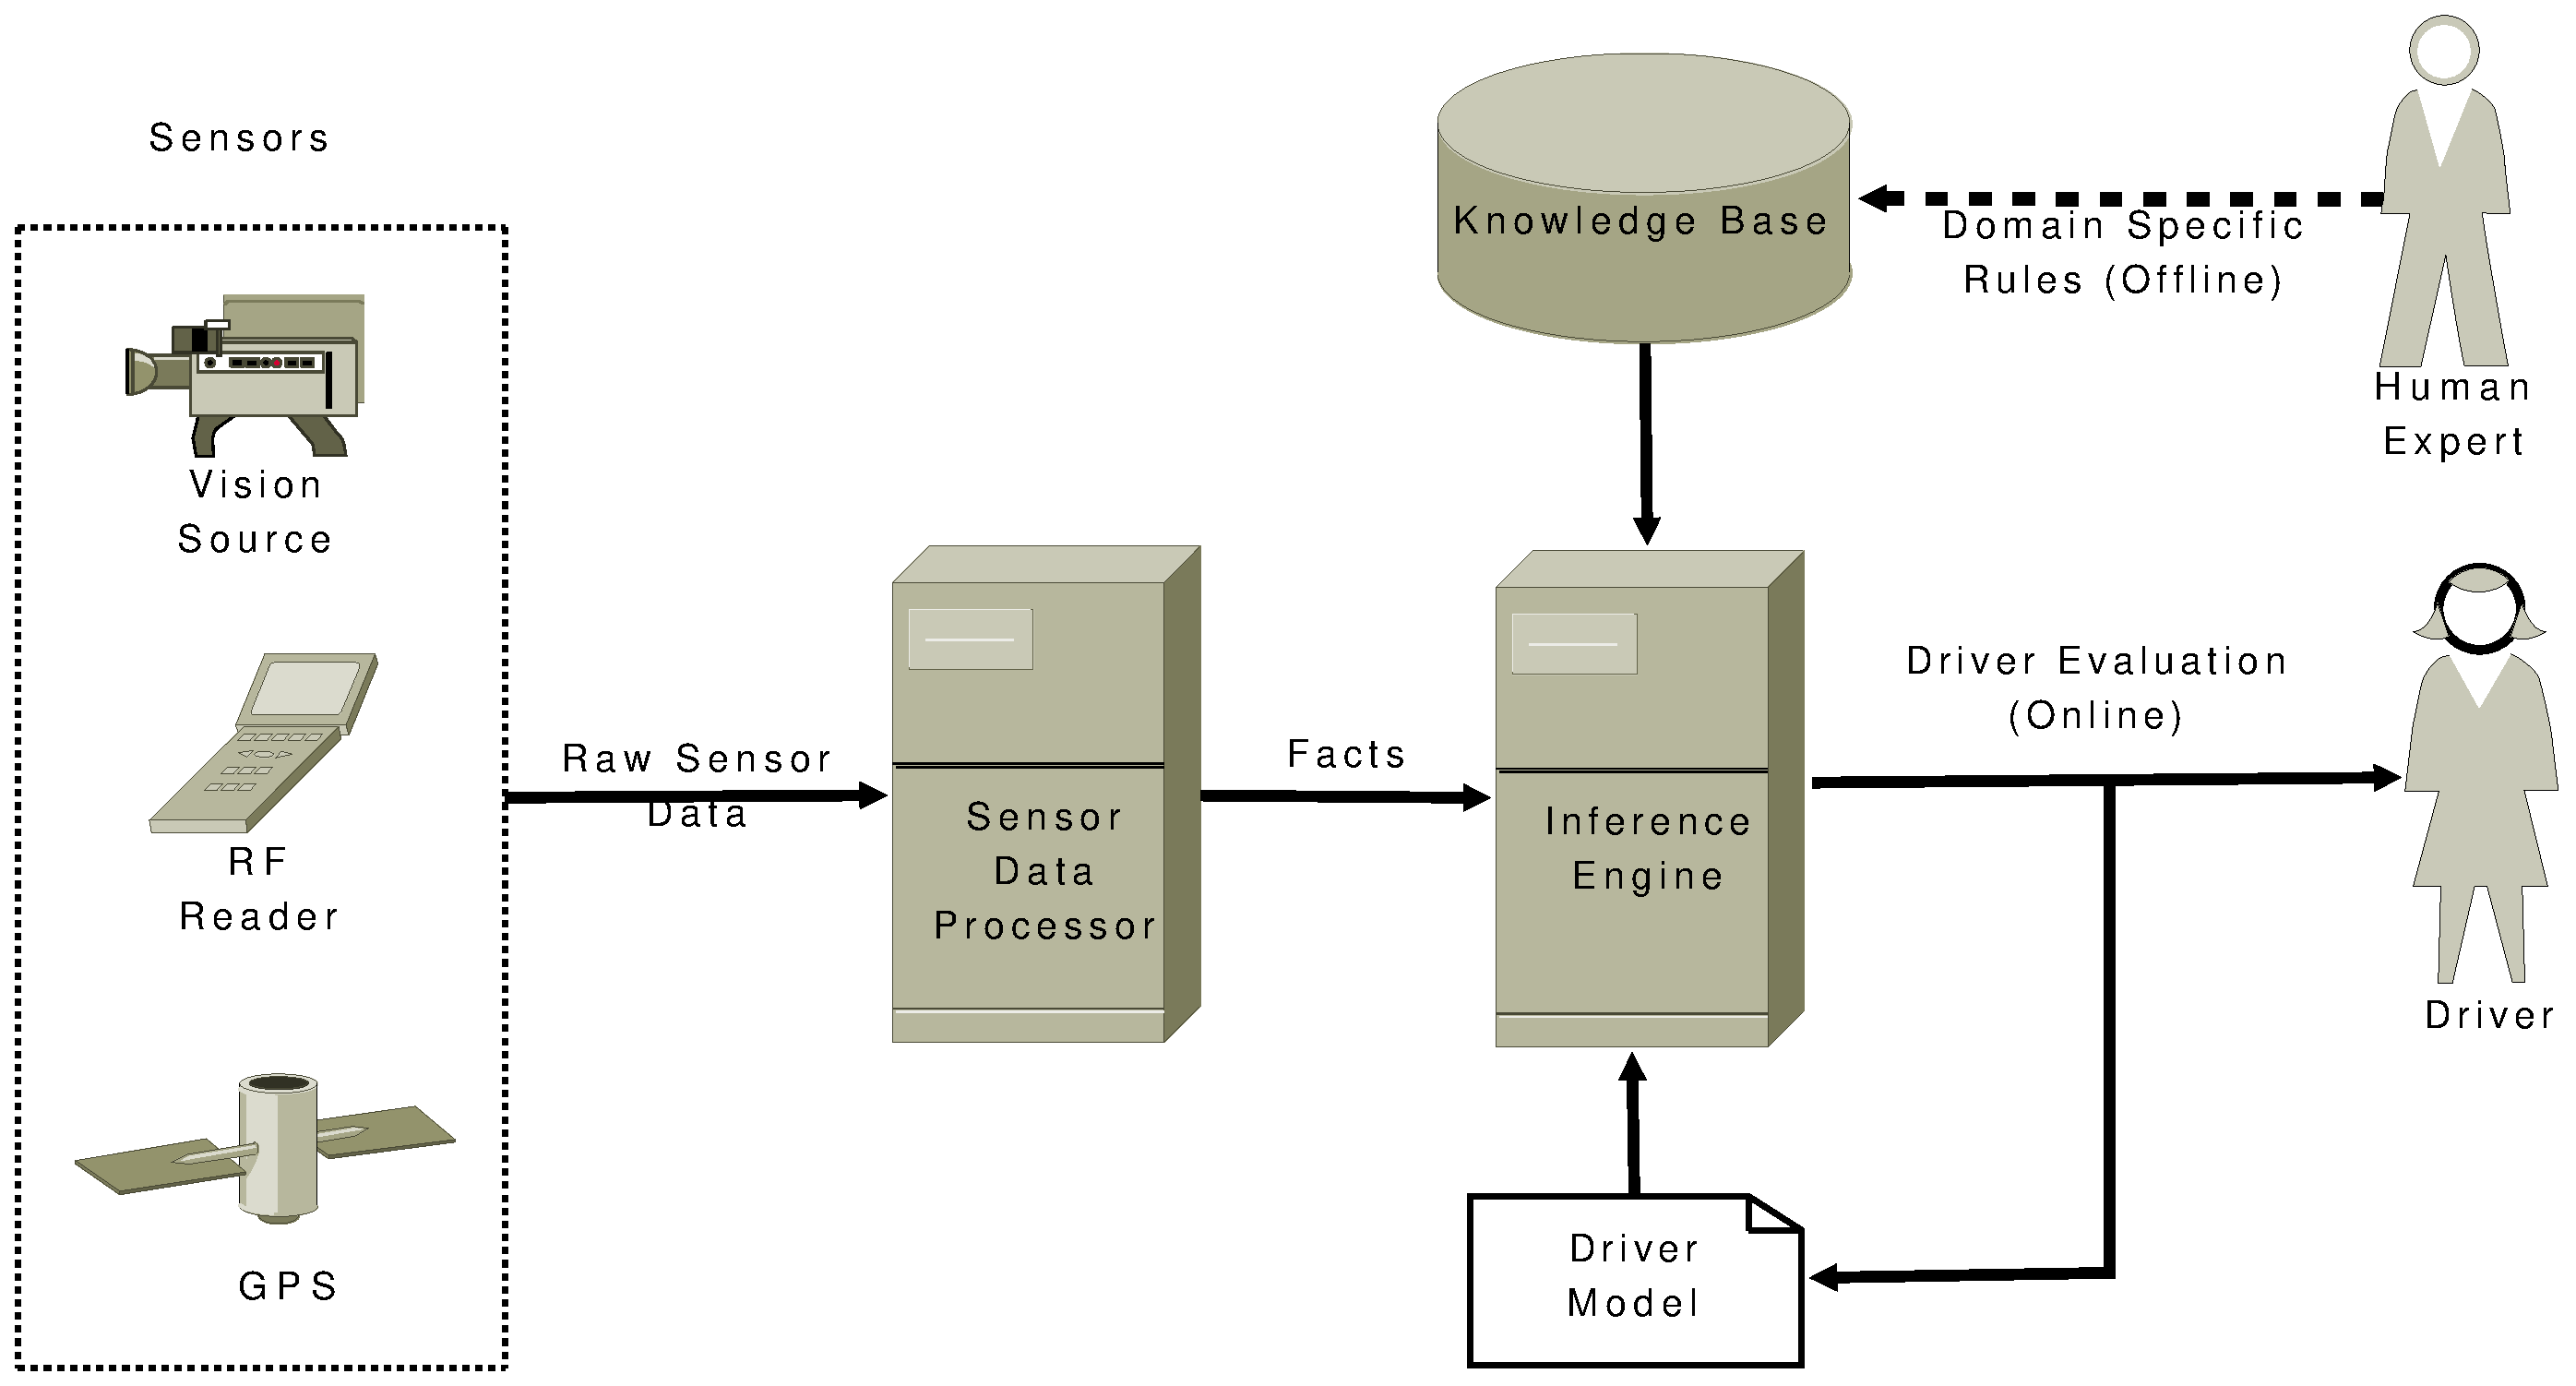
\includegraphics[width=90mm,height=45mm]{../img/sys3.eps}
  \caption{Basic system architecture of ADES project.}
  \label{fig:sys}
  \end{center}
  \end{figure}
}

\frame
{
  \frametitle{Data Acquisition and Processing}
  \begin{itemize}
  	\item Vision module
	  	\begin{itemize}
	  		\item Detection and tracking of lane markings.
	  		\item Detection, tracking, and recognition of traffic signs.
	  	\end{itemize}
		\item RFID system
		\item GPS/GIS system
		\item CAN-Bus integration
	\end{itemize}
}

\frame
{
  \frametitle{Inference Engine}
  \begin{itemize}
  	\item A common interface for expert system implementations
		\item Prolog Based
		\item Belief Networks Based
	\end{itemize}
	\begin{table}
	\caption{Targeted traffic rules.}
	\centering
	% Table generated by Excel2LaTeX from sheet 'tables'
	{\scriptsize
	\begin{tabular}{|l|r|}
	\hline
	{\bf Violation} & {\bf Fine} \\
	\hline
	Violating the red traffic light &     140 TL \\
	\hline
	Exceeding speed limits from 10 up to 30 percent &     140 TL \\
	\hline
	Exceeding speed limits more than 30 percent &     290 TL \\
	\hline
	Entering forbidden roads. &     140 TL \\\hline
	Not obeying the signs and land markings &      66 TL \\
	\hline
	\end{tabular} 
	}   
	\label{ceza}
	\end{table}
}


\section{METHODOLOGY}
\mysectionpage{METHODOLOGY}{METHODOLOGY}

\subsection{Vision Module}
\frame
{
  \frametitle{Overview}
  \begin{figure}[ht]
	\begin{center}
	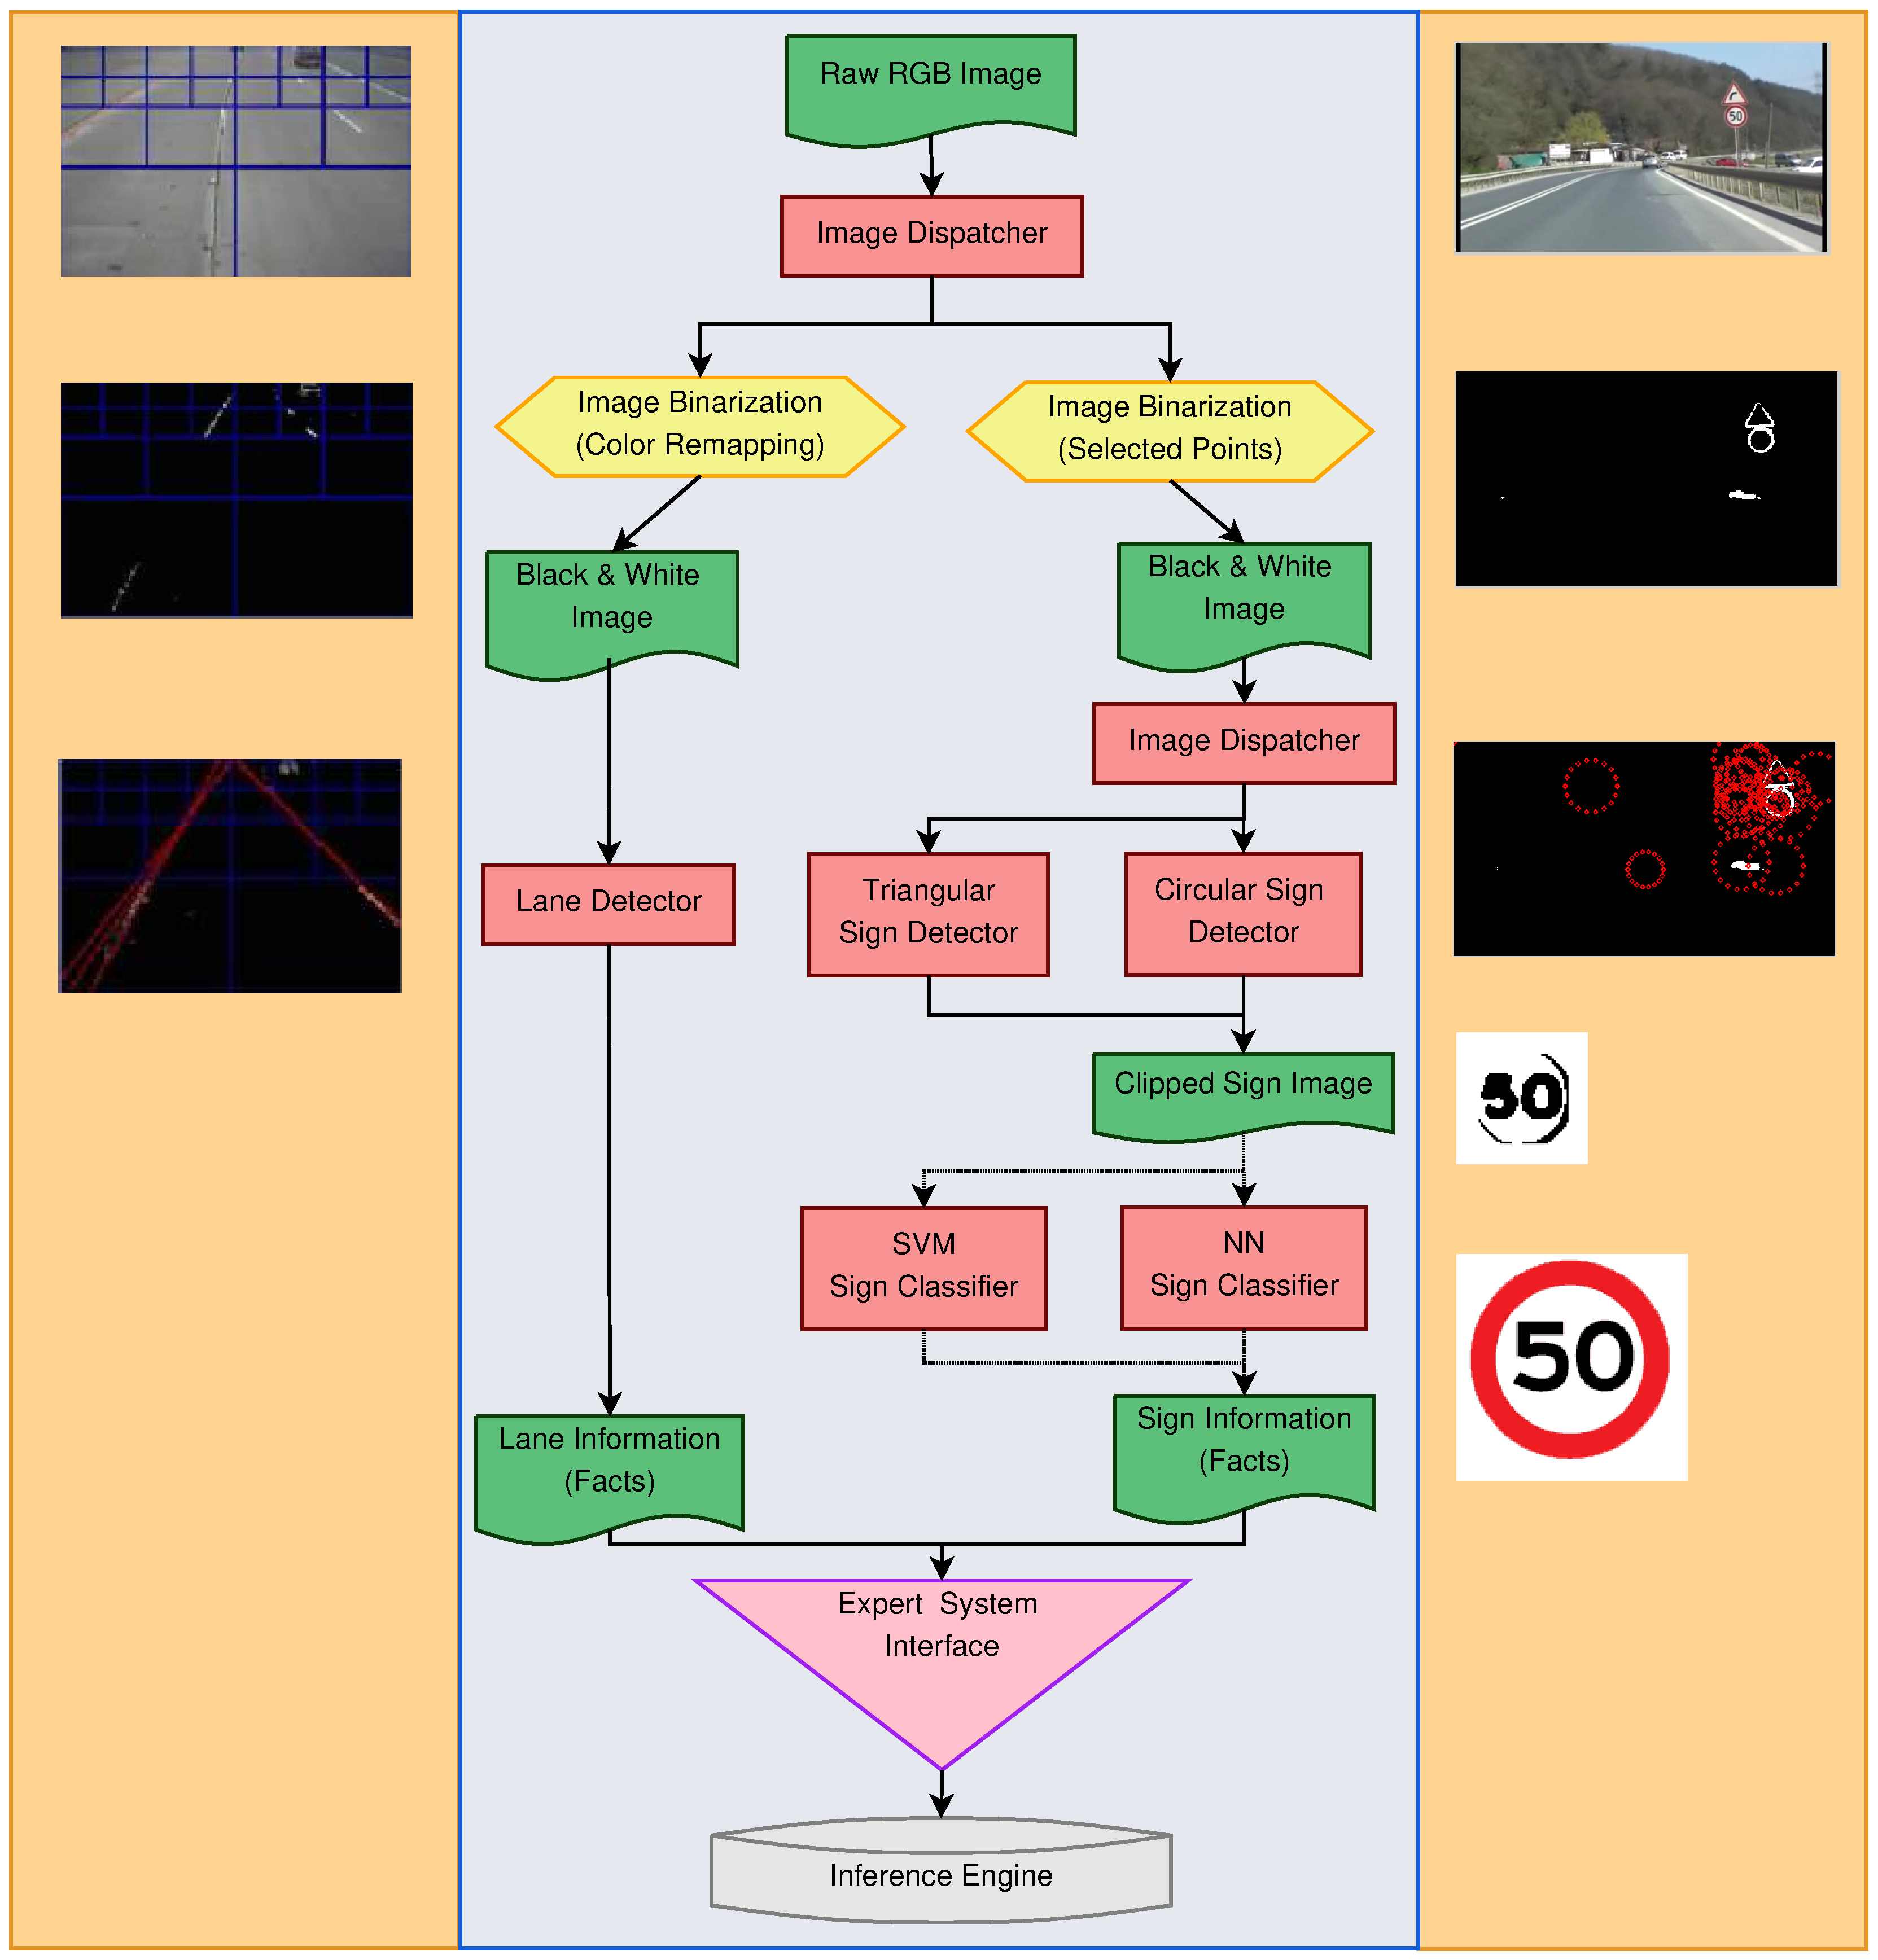
\includegraphics[height=.6\paperheight]{../img/vision.eps}
	\caption{Vision processing.}
	\label{fig:vision}
	\end{center}
	\end{figure}
}

\frame
{
  \frametitle{Image Binarization - Color Remapping}
	\begin{table}
	\caption{Color remapping.}
	\centering
	{\footnotesize
	% Table generated by Excel2LaTeX from sheet 'tables'
	\begin{tabular}{|r|r|r|r|}
	\hline
	{\bf Pixel Value} & {\bf Red} & {\bf Green} & {\bf Blue} \\
	\hline
	{\bf 0-176} & 0 & 0 & 0 \\
	\hline
	{\bf 176-196} & 1 & 1 & 0 \\
	\hline
	{\bf 196-255} & 1 & 1 & 1 \\
	\hline
	\end{tabular}  }  
	\label{tabldtable2}
	\end{table}
	\par
}

\frame
{
  \frametitle{Adaptive image binarization}
	\begin{eqnarray}
	\label{eq1}
	f(r,g,b)&=& \left\{\begin{array}{l} 1 \rightarrow r>\alpha \times g, r>\beta \times b \\ 
																			0 \rightarrow o/w \end{array}\right\}\\
	\nonumber \alpha &>& 1 \\
	\nonumber \beta &>& 1
	\end{eqnarray}
	
}

\frame
{
  \frametitle{Adaptive image binarization (cont'd)}
  \begin{figure}[ht]
	\begin{center}
	\includegraphics[height=.6\paperheight]{../img/hist1.eps}
	\caption{Good, medium and poor conditions for traffic sign detection.}
	\label{fig:hist1}
	\end{center}
	\end{figure}
}


\frame
{
	\frametitle{Adaptive image binarization (cont'd)}
	\vspace*{-2mm}
	{\footnotesize
	\begin{eqnarray}
	\label{eq2}
	HIST &=& Histogram(HSL_{rgb}) \\
	\nonumber \alpha = \beta &=& 1 + \frac {L_{mean}}{2}
	\end{eqnarray}
	A better approach is;
  \begin{eqnarray}
	\label{eq3}
	p_{i} &=& \left\{\begin{array}{l} 1 \rightarrow p=white \\ 0 \rightarrow p=black \end{array}\right\}\\
	\nonumber p_{white} &=& \sum{p_{i}}, \forall p \in image \\
	\nonumber \alpha &=& \left\{\begin{array}{l} \alpha \times \alpha' \rightarrow p_{white}>max_{white} \\ \frac{\alpha}{\alpha'}\rightarrow p_{white}<min_{white} \\ \alpha \rightarrow o/w \end{array}\right\}, \alpha'>1\\
	\nonumber \beta &=& \left\{\begin{array}{l} \beta \times \beta' \rightarrow p_{white}>max_{white} \\ \frac{\beta}{\beta'}\rightarrow p_{white}<min_{white} \\ \beta \rightarrow o/w \end{array}\right\}, \beta'>1
	\end{eqnarray}
	}
}

\frame
{
	\frametitle{Adaptive image binarization (cont'd)}
	\begin{figure}[ht]
	\begin{center}
	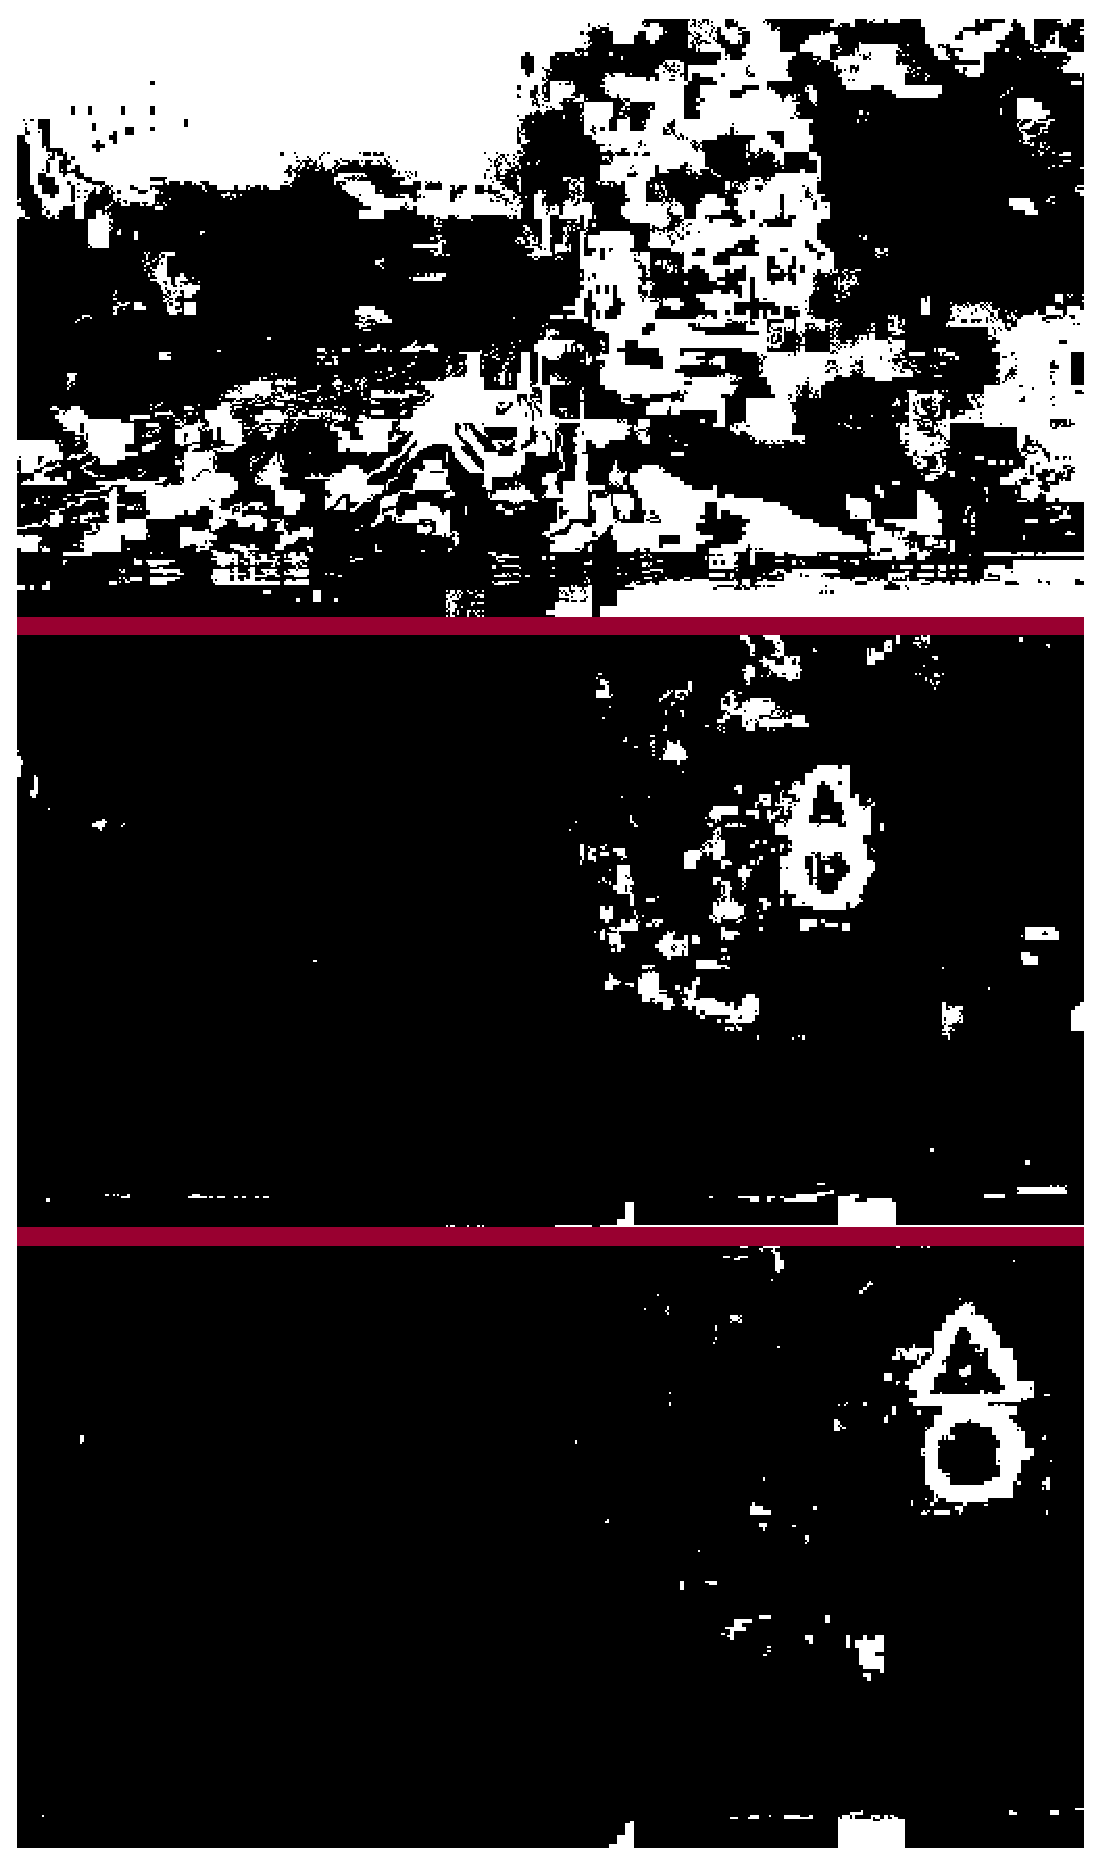
\includegraphics[height=.6\paperheight]{../img/adapbright.eps}
	\caption{Effect of selected point count on image binarization.}
	\label{fig:adapbright}
	\end{center}
	\end{figure}
}


\frame
{
	\frametitle{Road Lane Detection}
	\begin{figure}[ht]
	\begin{center}
	\includegraphics[width=.8\paperwidth]{../img/ldfig1.eps}
	\caption{(a) Partitioned image, (b) Binary image.}
	\label{fig:ldfig1}
	\end{center}
	\end{figure}
	\par
}

\frame
{
	\frametitle{Road Lane Detection (cont'd)}
	\begin{figure}[ht]
	\begin{center}
	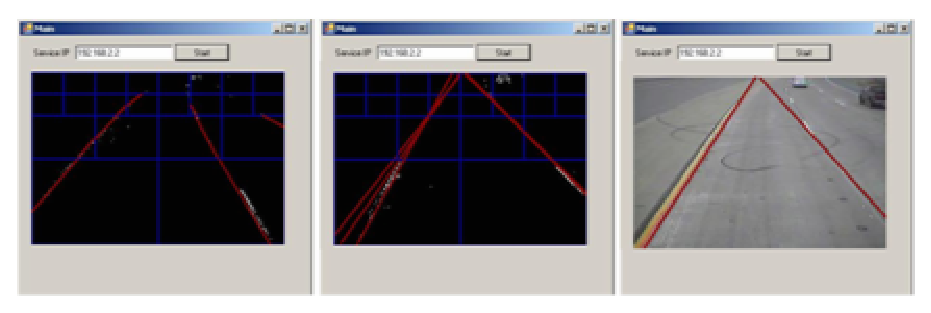
\includegraphics[width=.8\paperwidth]{../img/ldfig2.eps}
	\caption{(a) Candidate lines, (b) Transformed line, (c) Detected lines.}
	\label{fig:ldfig2}
	\end{center}
	\end{figure}
}

\frame
{
	\frametitle{Road Lane Detection (cont'd)}
	Translation function for Hough Lines;
	\begin{equation} 
	\label{eq4} 
	\begin{array}{l} {r'\, \, =\, r+(x-x')\cos (\theta )+(y-y')\sin (\theta )} \\ {\theta '=\, \theta } \end{array} 
	\end{equation}
}

\frame
{
	\frametitle{Road Lane Tracking}
	\begin{table}
	\caption{(a) Transmission matrix for \textit{r}, (b) Transmission matrix for \textit{$\theta $}.}
	\centering
	{\tiny
	\begin{tabular}{|r|r|r|r|r|r|r|r|r|r|}
	\hline
	{\bf {\normalsize $r$}} & {\bf 0} & {\bf 1} & {\bf 2} & {\bf 3} & ... & {\bf 279} & {\bf 280} & {\bf 281} & {\bf 282} \\
	\hline
	{\bf 0} & 0,3989 & 0,2420 & 0,0540 & 0,0044 & ... & 0,0000 & 0,0000 & 0,0000 & 0,0000 \\
	\hline
	{\bf 1} & 0,2420 & 0,3989 & 0,2420 & 0,0540 & ... & 0,0000 & 0,0000 & 0,0000 & 0,0000 \\
	\hline
	{\bf 2} & 0,0540 & 0,2420 & 0,3989 & 0,2420 & ... & 0,0000 & 0,0000 & 0,0000 & 0,0000 \\
	\hline
	... & ... & ... & ... & ... & ... & ... & ... & ... & ... \\
	\hline
	{\bf 280} & 0,0000 & 0,0000 & 0,0000 & 0,0000 & ... & 0,2420 & 0,3989 & 0,2420 & 0,0540 \\
	\hline
	{\bf 281} & 0,0000 & 0,0000 & 0,0000 & 0,0000 & ... & 0,0540 & 0,2420 & 0,3989 & 0,2420 \\
	\hline
	{\bf 282} & 0,0000 & 0,0000 & 0,0000 & 0,0000 & ... & 0,0044 & 0,0540 & 0,2420 & 0,3989 \\
	\hline
	\multicolumn{10}{c}{} \\
	\hline
	{\bf {\normalsize $\theta$}} & {\bf 0} & {\bf 1} & {\bf 2} & {\bf 3} & ... & {\bf 176} & {\bf 177} & {\bf 178} & {\bf 179} \\
	\hline
	{\bf 0} & 0,3989 & 0,2420 & 0,0540 & 0,0044 & ... & 0,0001 & 0,0044 & 0,0540 & 0,2420 \\
	\hline
	{\bf 1} & 0,2420 & 0,3989 & 0,2420 & 0,0540 & ... & 0,0000 & 0,0001 & 0,0044 & 0,0540 \\
	\hline
	{\bf 2} & 0,0540 & 0,2420 & 0,3989 & 0,2420 & ... & 0,0000 & 0,0000 & 0,0001 & 0,0044 \\
	\hline
	... & ... & ... & ... & ... & ... & ... & ... & ... & ... \\
	\hline
	{\bf 177} & 0,0044 & 0,0001 & 0,0000 & 0,0000 & ... & 0,2420 & 0,3989 & 0,2420 & 0,0540 \\
	\hline
	{\bf 178} & 0,0540 & 0,0044 & 0,0001 & 0,0000 & ... & 0,0540 & 0,2420 & 0,3989 & 0,2420 \\
	\hline
	{\bf 179} & 0,2420 & 0,0540 & 0,0044 & 0,0001 & ... & 0,0044 & 0,0540 & 0,2420 & 0,3989 \\
	\hline
	\end{tabular}  
	}
	\label{tab:ldtable3}
	\end{table}	
}

\frame
{
	\frametitle{Road Lane Tracking (cont'd)} 
	\begin{table}
	\caption{(a) Emission matrix for \textit{r}, (b) Emission matrix for \textit{$\theta $}.}
	\centering
	{\tiny
	\begin{tabular}{|r|r|r|r|r|r|r|r|r|r|}
	\hline
	{\bf {\normalsize $r$}} & {\bf 0} & {\bf 1} & {\bf 2} & {\bf 3} & {\bf 4} & {\bf 5} & {\bf ...} & {\bf 281} & {\bf 282} \\
	\hline
	{\bf 0} & 0,1995 & 0,1760 & 0,1210 & 0,0648 & 0,0270 & 0,0088 & ... & 0,0000 & 0,0000 \\
	\hline
	{\bf 1} & 0,1760 & 0,1995 & 0,1760 & 0,1210 & 0,0648 & 0,0270 & ... & 0,0000 & 0,0000 \\
	\hline
	{\bf 2} & 0,1210 & 0,1760 & 0,1995 & 0,1760 & 0,1210 & 0,0648 & ... & 0,0000 & 0,0000 \\
	\hline
	{\bf 3} & 0,0648 & 0,1210 & 0,1760 & 0,1995 & 0,1760 & 0,1210 & ... & 0,0000 & 0,0000 \\
	\hline
	{\bf 4} & 0,0270 & 0,0648 & 0,1210 & 0,1760 & 0,1995 & 0,1760 & ... & 0,0000 & 0,0000 \\
	\hline
	... & ... & ... & ... & ... & ... & ... & ... & ... & ... \\
	\hline
	{\bf 281} & 0,0000 & 0,0000 & 0,0000 & 0,0000 & 0,0000 & 0,0000 & ... & 0,1995 & 0,1760 \\
	\hline
	{\bf 282} & 0,0000 & 0,0000 & 0,0000 & 0,0000 & 0,0000 & 0,0000 & ... & 0,1760 & 0,1995 \\
	\hline
	\multicolumn{10}{c}{} \\
	\hline
	{\bf {\normalsize $\theta$}} & {\bf 0} & {\bf 1} & {\bf 2} & {\bf 3} & {\bf 4} & {\bf 5} & {\bf ...} & {\bf 178} & {\bf 179} \\
	\hline
	{\bf 0} & 0,1995 & 0,1760 & 0,1210 & 0,0648 & 0,0270 & 0,0088 & ... & 0,1210 & 0,1760 \\
	\hline
	{\bf 1} & 0,1760 & 0,1995 & 0,1760 & 0,1210 & 0,0648 & 0,0270 & ... & 0,0648 & 0,1210 \\
	\hline
	{\bf 2} & 0,1210 & 0,1760 & 0,1995 & 0,1760 & 0,1210 & 0,0648 & ... & 0,0270 & 0,0648 \\
	\hline
	{\bf 3} & 0,0648 & 0,1210 & 0,1760 & 0,1995 & 0,1760 & 0,1210 & ... & 0,0088 & 0,0270 \\
	\hline
	{\bf 4} & 0,0270 & 0,0648 & 0,1210 & 0,1760 & 0,1995 & 0,1760 & ... & 0,0022 & 0,0088 \\
	\hline
	... & ... & ... & ... & ... & ... & ... & ... & ... & ... \\
	\hline
	{\bf 178} & 0,1210 & 0,0648 & 0,0270 & 0,0088 & 0,0022 & 0,0004 & ... & 0,1995 & 0,1760 \\
	\hline
	{\bf 179} & 0,1760 & 0,1210 & 0,0648 & 0,0270 & 0,0088 & 0,0022 & ... & 0,1760 & 0,1995 \\
	\hline
	\end{tabular} 
	} 
	\label{tab:ldtable4}
	\end{table}
}

\frame
{
  \frametitle{Traffic Sign Detection}
  \begin{block}{Affine transformation}
  is any transformation that preserves collinearity and ratios of distances. (MathWorld)
  \end{block}
  \begin{eqnarray}
	\label{eq5}
	\left| \begin{array}{ccc} u' \\ v' \\ w \end{array} \right| &=& 
	\left| \begin{array}{ccc} a & b & c \\ d & e & f \\ g & h & 1 \end{array} \right| \left| \begin{array}{ccc} x \\ y \\ 1 \end{array} \right| \\
	\nonumber u &=& u'/w \\
	\nonumber v &=& v'/w 
	\end{eqnarray}
}

\frame
{
  \frametitle{Traffic Sign Detection (cont'd)}
  For example;
  \begin{eqnarray}
  \label{eq6}
	\left| \begin{array}{ccc} u' \\ v' \\ 1 \end{array} \right| &=& 
	\left| \begin{array}{ccc} 2 & 1 & 100 \\ 1 & 2 & 50 \\ 0 & 0 & 1 \end{array} \right| \left| \begin{array}{ccc} x \\ y \\ 1 \end{array} \right|
	\end{eqnarray}

}

\frame
{
  \frametitle{Traffic Sign Detection (cont'd)}
  \begin{figure}[ht]
	\begin{center}
	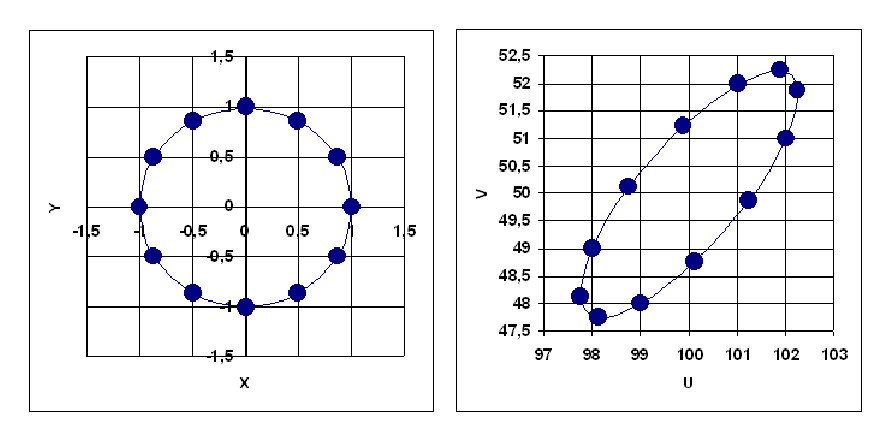
\includegraphics[width=.8\paperwidth]{../img/sdfig6.eps}
	\caption{Template characteristic points in (x,y) domain,  and (u,v) domain after geometric transformation.}
	\label{fig:sdfig6}
	\end{center}
	\end{figure}
}

\frame
{
  \frametitle{Traffic Sign Detection (cont'd)}
	\begin{figure}[ht]
	\begin{center}
	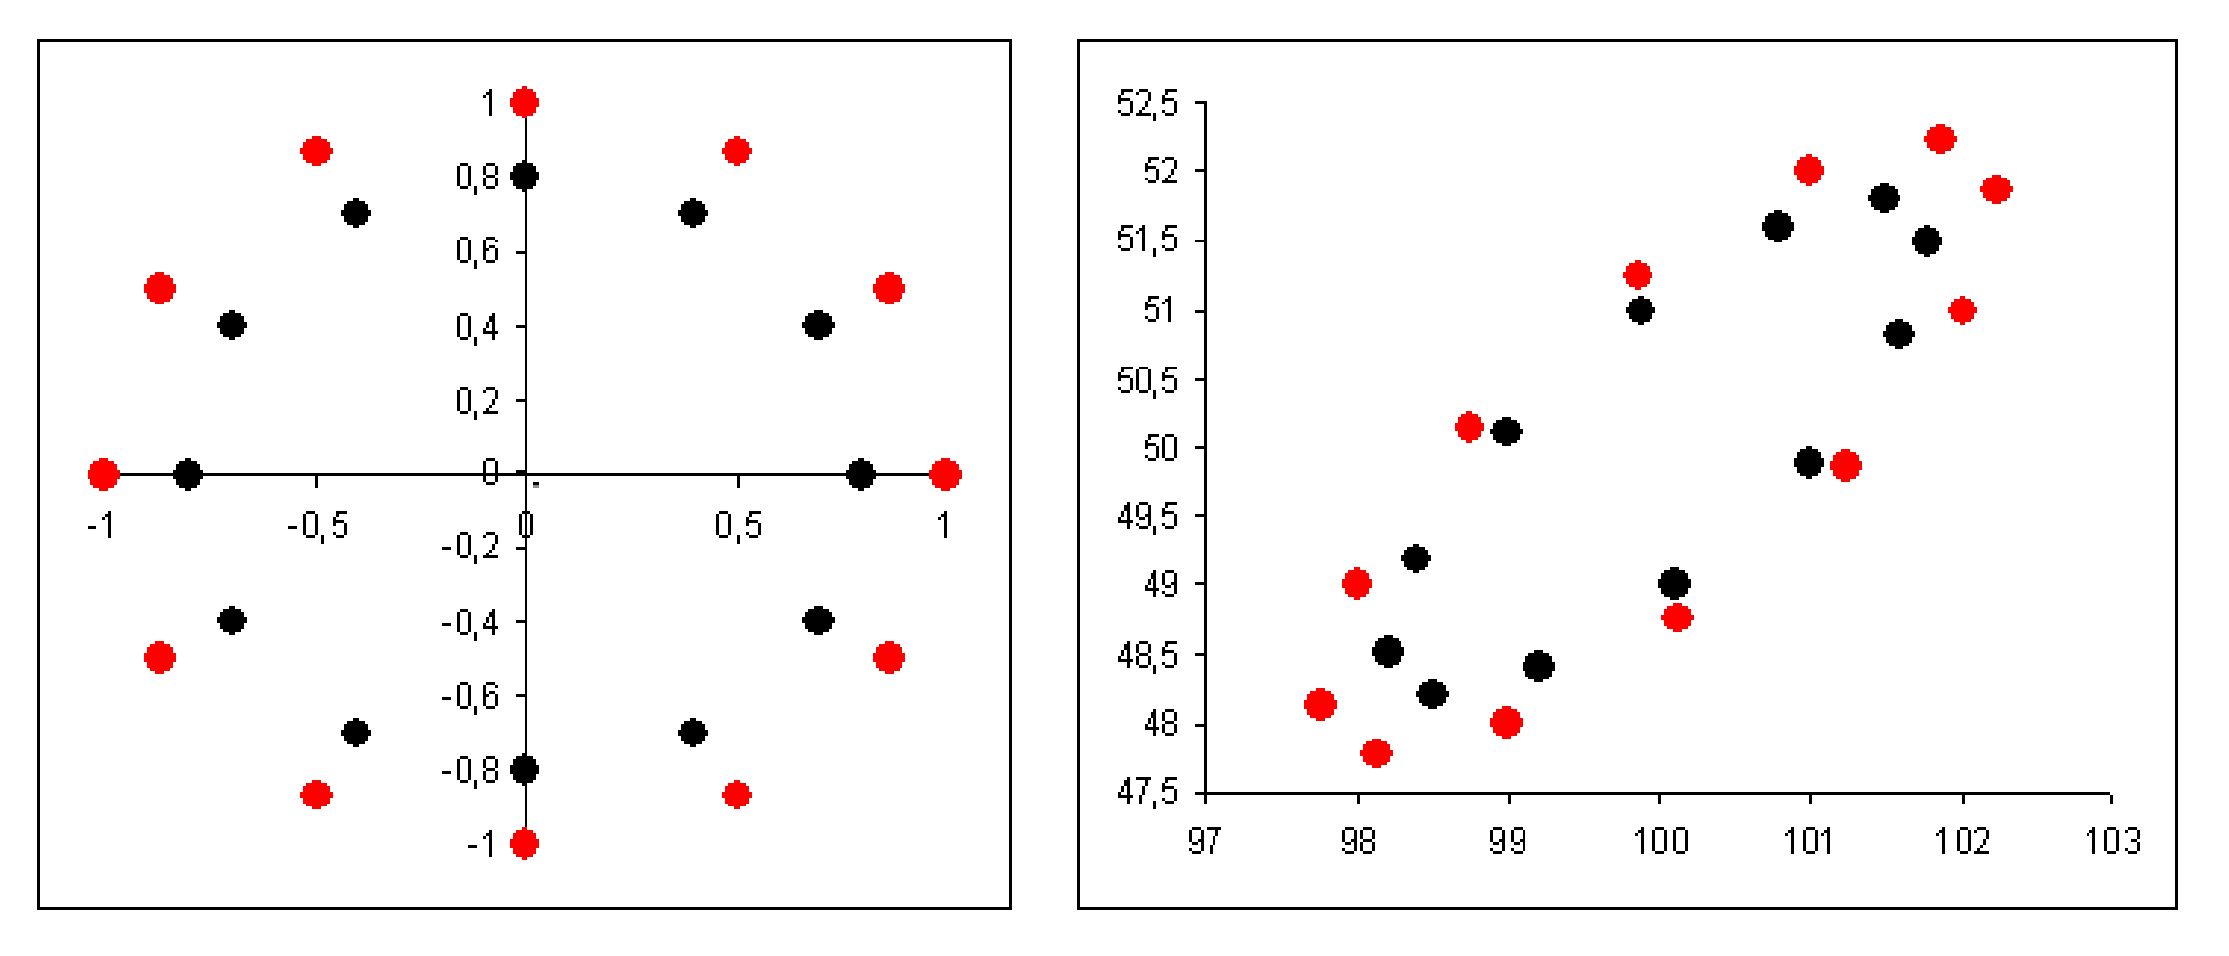
\includegraphics[width=.8\paperwidth]{../img/sdfig7.eps}
	\caption{Red and non-red template points.}
	\label{fig:sdfig7}
	\end{center}
	\end{figure}
}


\frame
{
	In our implementation;
  \frametitle{Traffic Sign Detection (cont'd)}
  \begin{eqnarray}
	\label{eq7}
	\left| \begin{array}{ccc} u \\ v \\ 1 \end{array} \right| &=& 
	\left| \begin{array}{ccc} a & 0 & c \\ 0 & a & f \\ 0 & 0 & 1 \end{array} \right| \left| \begin{array}{ccc} x \\ y \\ 1 \end{array} \right|
	\end{eqnarray}
}

\frame
{
  \frametitle{Traffic Sign Detection (cont'd)}
  Crossover function:
  \begin{eqnarray}
	\label{eq8}
	\nonumber a_{newchromosome}&=&\alpha.a_{chromosome1}+\beta.a_{chromosome2} \\
	c_{newchromosome}&=&\alpha.c_{chromosome1}+\beta.c_{chromosome2} \\
	\nonumber f_{newchromosome}&=&\alpha.f_{chromosome1}+\beta.f_{chromosome2} \\
	\nonumber 1&=&\alpha+\beta
	\end{eqnarray}
}

\frame
{
  \frametitle{Traffic Sign Detection (cont'd)}
	GA individuals;
	\begin{figure}[ht]
	\begin{center}
	\includegraphics[height=.3\paperheight]{../img/sdfig3.eps}
	\includegraphics[height=.3\paperheight]{../img/sdfig4.eps}
	\caption{Initial and converged chromosomes.}
	\label{fig:sdfig4}
	\end{center}
	\end{figure}
	A Modified Radial Symmetry check is performed after GA detection.	
}

\frame
{
  \frametitle{Traffic Sign Detection (cont'd)}
  \begin{figure}[ht]
	\begin{center}
	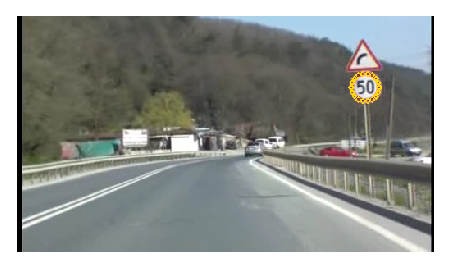
\includegraphics[width=.8\paperwidth]{../img/sdfig5.eps}
	\caption{Detected traffic sign.}
	\label{fig:sdfig5}
	\end{center}
	\end{figure}
}

\frame
{
  \frametitle{Traffic Sign Classification}
	\begin{figure}[ht]
	\begin{center}
	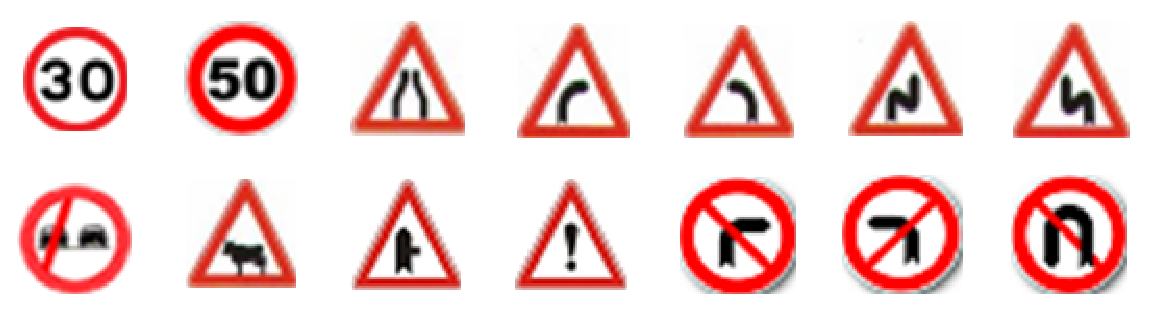
\includegraphics[width=.8\paperwidth]{../img/signs_vertical.eps}
	\caption{Traffic signs recognized by the proposed system.}
	\label{fig:signs}
	\end{center}
	\end{figure}	
}

\frame
{
  \frametitle{Traffic Sign Classification (cont'd)}
  Grid based feature selection;
	\begin{figure}[ht]
	\begin{center}
	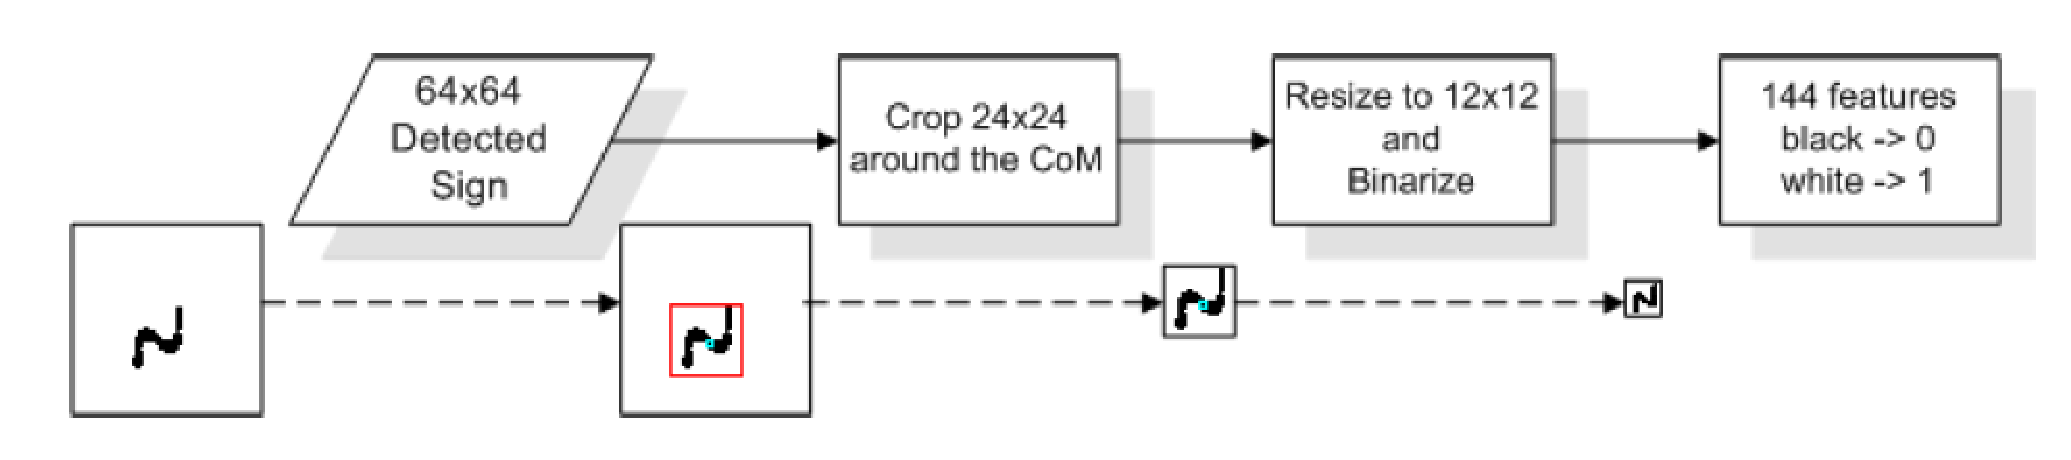
\includegraphics[width=.8\paperwidth]{../img/nn12.eps}
	\caption{Input array formation for Grid based NN and SVM implementations.}
	\end{center}
	\end{figure}
}

\frame
{
  \frametitle{Traffic Sign Classification (cont'd)}
  Surf based feature selection;
	\begin{figure}[ht]
	\begin{center}
	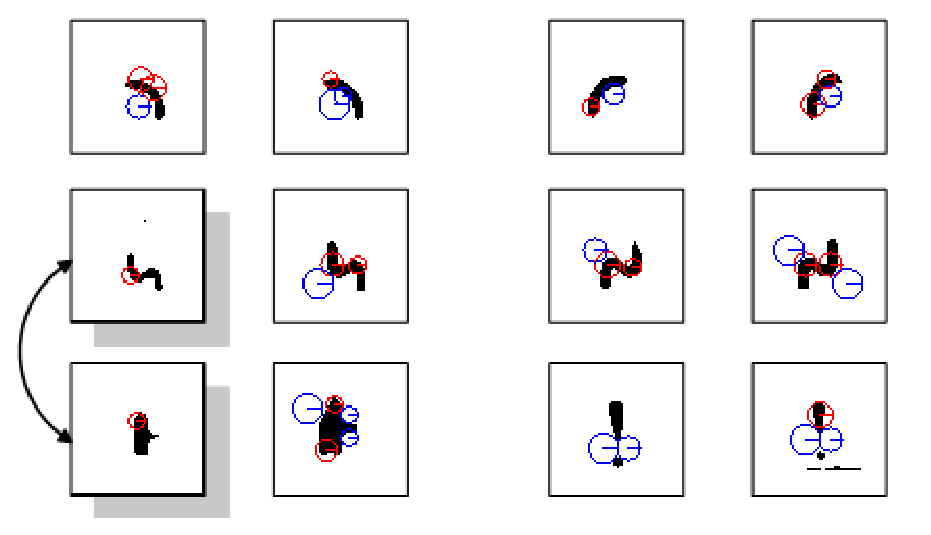
\includegraphics[width=.8\paperwidth]{../img/surf.eps}
	\caption{U-SURF results for different sign types (octaves=3, intervals=5).}
	\end{center}
	\end{figure}
}

\frame
{
  \frametitle{Traffic Sign Classification (cont'd)}
  In the NN implementation;
  \begin{itemize}
    \item A separate network for each sign.
 		\item Each network has one hidden layer with four nodes (144x4x1)
  	\item NN implementation with Levenberg-Marquardt learning technique.
  \end{itemize}
	\begin{eqnarray}
	\label{eq9}
		(J^{t}J + \lambda I)\phi &=& J^{t}E
	\end{eqnarray}  
}

\frame
{
  \frametitle{Traffic Sign Classification (cont'd)}
  In the SVM implementation, the RBF kernel function is used.
  \begin{eqnarray}
	\label{eq10}
		k(u,v) &=& e^{-\gamma \times |u-v|^2}
	\end{eqnarray}
}


\subsection{RF Module, GPS/GIS and CAN Bus}
\frame
{
  \frametitle{Properties of Most Common RFID Systems}
  \begin{table}
	\caption{Properties of most common RFID systems.}
	\centering
	{\tiny
	\begin{tabular}{|p{18mm}|p{18mm}|p{18mm}|p{18mm}|p{18mm}|}
	\hline
	{\bf Band} & {\bf Low Frequency} & {\bf High Frequency} & {\bf Ultra-High Frequency} & {\bf Microwave} \\
	\hline
	{\bf Typical RFID Frequencies} & 125-134 kHz &  13.56 MHz & 433, 865-956 MHz &   2.45 MHz \\
	\hline
	{\bf Read Range} &     \textless 0.5m &     \textless 1.5m &       \textless 5m &      \textless 10m \\
	\hline
	{\bf Data Transfer Rate} &   1 kbit/s &  25 kbit/s & 30-100 kbits/s & \textless 100 kbit/s \\
	\hline
	{\bf Sample Application} & Car Immobilizer & Contact-less travel cards &  Logistics & Electronic toll collection \\
	\hline
	\end{tabular} 
	}
	\label{tab:rfid1}
	\end{table}
}

\frame
{
  \frametitle{Challenges of RFID Technology}
	\begin{itemize}
		\item Power consumption
		\item Reading range
		\item Antenna
		\item Metal interference
		\item Passive tag limitations
	\end{itemize}	
}

\frame
{
  \frametitle{Tag ID Assignment}
	\begin{table}%
	\caption{Tag ID assignment strategy.}
	% Table generated by Excel2LaTeX from sheet 'Sayfa1'
	{\tiny
	\begin{tabular}{|r|p{10mm}|p{30mm}|r|}
	\hline
	{\bf Tag Part} & {\bf Length (Bytes)} & {\bf Explanation} & {\bf Example} \\
	\hline
	  UniqueID &          4 & Latitude and Longitude & 41.013144-29.081244 \\
	\hline
	    RuleID &          1 & Predefined Rule ID & 13 (no trun left) \\
	\hline
	Pre/Post/Single &          1 & Type of Tag & Pre - no turn left \\
	\hline
	Matching Tag ID &          1 & Matching Tag for pre/post tags  & UniqueID of pre tag for a post tag \\
	\hline
	       CRC &          1 & Redundancy Check &   01010101 \\
	\hline
	           & {\bf Total: 8 bytes} &            &            \\
	\hline
	\end{tabular} 
	}
	\label{tagid}
	\end{table}
}

\subsection{GIS/GPS and CAN-Bus}
\begin{frame}[fragile]
	\frametitle{Simple GIS for ADES}
	\begin{figure}[!ht]
  \centering
	\begin{mylisting}
	\begin{verbatim}
		<?xml version="1.0" encoding="utf-8" ?>
		<GIS>
		  <NodeProp lat="0,0.04,N" lon="0,0.00,W" rule="1"/>
		  <NodeProp lat="0,0.12,N" lon="0,0.00,W" rule="13" 
		    type="pre" matching="0,0.12,N:0,0.00,W"/>
		  <NodeProp lat="0,0.13,N" lon="0,0.02,W" rule="13" 
		    type="post" matching="0,0.12,N:0,0.00,W"/>
		</GIS>
	\end{verbatim}
	\end{mylisting}
	\caption{Simple GIS XML for ADES.}
	\label{gisxml}
	\end{figure}
\end{frame}

\frame
{
	\frametitle{CAN Bus}
	Control Area Network (CAN) is a serial communications protocol. 
	\begin{itemize}
	\item Developed by Robert Bosch GmbH. 
	\item Supports distributed real-time control with a high level of security. 
	\item There are many ADAS applications which uses CAN bus integration.
	\item Provides speed of the vehicle and sensor readings from throttle, break, and steering control units.
	\end{itemize}
}

\subsection{Inference Engine}
\frame
{
	\frametitle{Properties of Rule Based and Probabilistic ES}
	\begin{table}
	\caption{Properties of expert system models.}
	\centering
	{\tiny
	\begin{tabular}{|p{30mm}|p{30mm}|p{30mm}|}
	\hline
	 & {\bf Probabilistic Model} & {\bf Rule Based Model} \\
	\hline
	{\bf Knowledge Base} & Probabilistic Structure,  Facts & Rules, Facts \\
	\hline
	{\bf Inference Engine} & Conditional probability evaluation (Bayes theorem) & Backward chaining, Forward chaining \\
	\hline
	{\bf Explanation Subsystem} & Based on conditional probabilities & Based on triggered rules \\
	\hline
	{\bf Learning Subsystem} & Change in probabilistic structure and probabilities & Adding, removing rules \\
	\hline
	\end{tabular}
	}
	\label{tabESprop}
	\end{table}
}

\frame
{
	\frametitle{Comparison of Rule based and Probabilistic ES}
	\begin{table}
	\caption{Comparison of expert systems models.}
	\centering
	{\tiny
	\begin{tabular}{|p{30mm}|p{30mm}|p{30mm}|}
	\hline
	 & {\bf Probabilistic Model} & {\bf Rule Based Model} \\
	\hline
	{\bf Advantages} & Easy learning, Easy probability propagation & Easy explanation, Easy modification \\
	\hline
	{\bf Shortcomings} & High number of parameters & Performance issues, Certainty implementation \\
	\hline
	\end{tabular}  
	}
	\label{tabESComp}
	\end{table}
}

\begin{frame}[fragile]
	\frametitle{ADES Interface for Expert Systems}
  \begin{figure}[!ht]
  \centering
  \begin{mylisting}
	\begin{verbatim}
	public interface ExpertSystems
        {
            string init(params object[] esParams);
            string assertFact(params object[] esParams);
            string retractFact(params object[] esParams);
            string[] query(params object[] esParams);
            void setThreshold(double threshold);
            double getThreshold();
        }
	\end{verbatim}
	\end{mylisting}
  \caption{ADES Interface for Expert Systems}
  \label{fig:interface}
  \end{figure}
\end{frame}


\frame
{
	\frametitle{Implementation with Prolog}
	Prolog 
	\begin{itemize}
	\item is a programming language for symbolic computation,
	\item suitable for solving problems which contains objects and relations,
	\item benefits from rule-based programming, built-in pattern matching and backtracking execution,
	\item is not similar to a conventional programming language.
	\end{itemize}	
}

\begin{frame}[fragile]
	\frametitle{Probabilistic Prolog}
	Classical approach for dealing with uncertainty;
  ~\\~
	\begin{mylisting}
		Rules and Facts
		\vspace*{2px}\hrule
		\begin{verbatim}
		weather(fine,P) :- sky(sunny,PS),temp(high,PT),P is PS*PT.
		sky(sunny,0.8).
		temp(high,0.9).
		\end{verbatim}
		
		Query
		\vspace*{2px}\hrule
		\begin{verbatim}
		?- weather(X,P).
		X = fine
		P = 0.72 (0,016 sec)
		\end{verbatim}
	\end{mylisting}
  ~\\~
	Extra handling for probability values is required.
\end{frame}

\begin{frame}[fragile]
	\frametitle{Probabilistic Prolog (cont'd)}
	Our approach;
  ~\\~
	\begin{mylisting}
		Rules and Facts
		\vspace*{2px}\hrule
		\begin{verbatim}
		weather(fine):-sky_sunny,temp_high.
		"0.8::sky_sunny".
		"0.9::temp_high".
		\end{verbatim}
		
		Query
		\vspace*{2px}\hrule
		\begin{verbatim}
		?- weather(X).
		Prob for sky_sunny is 0,8
		Prob for temp_high is 0,9
		Prob for this answer:0,72
		X = fine (0,000 sec)
		\end{verbatim}
	\end{mylisting}
	~\\~
	Probability values are coupled with facts.
\end{frame}
	

\begin{frame}[fragile]
	\frametitle{Probabilistic Prolog - Path Finding Example}
	Consider the following graph with probability values assigned to its edges.
	\begin{figure}[ht]
	\begin{center}
	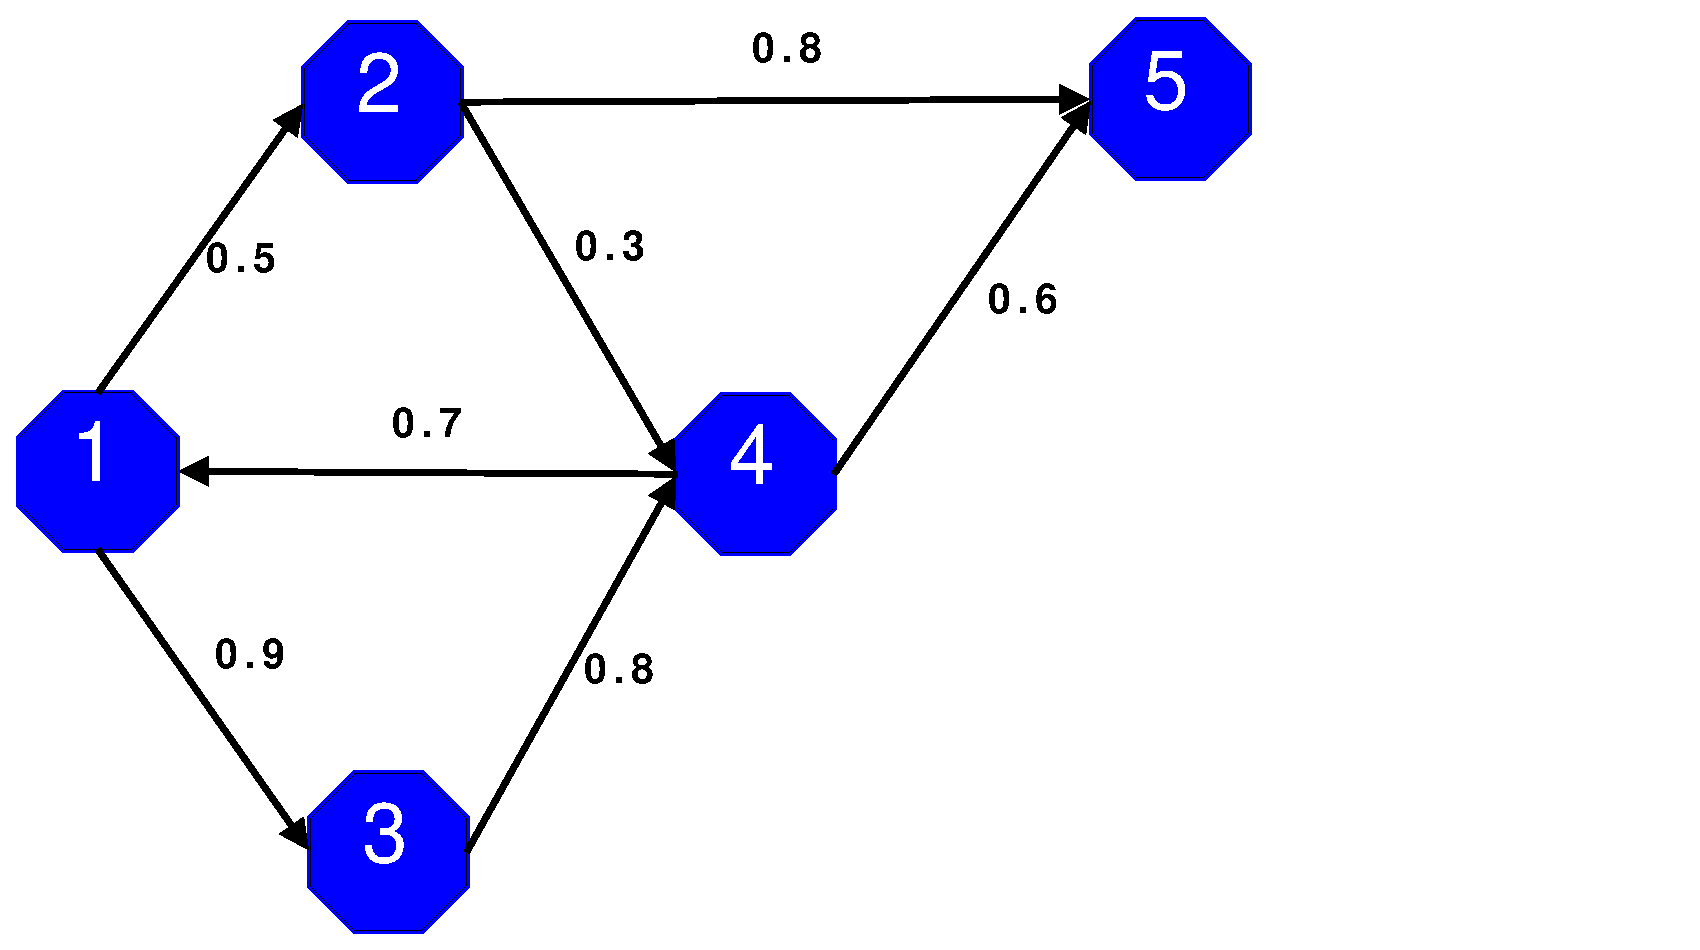
\includegraphics[width=.6\paperwidth]{../img/graph.eps}
	\caption{Directed graph with probability values.}
	\label{fig:graph}
	\end{center}
	\end{figure}
\end{frame}

\begin{frame}[fragile]
	\frametitle{Probabilistic Prolog - Path Finding Example (cont'd)}
	\begin{mylisting}
	Rules and Facts
	\vspace*{2px}\hrule
	\begin{verbatim}
	path(X,Y,[X|NL]) :- pathX(X,Y,L), reverse(L,[],NL), 
                      notvisited(X,NL).
	pathX(X,Y,L) :- pathX(X,Y,_,L).
	pathX(X,X,A,A).
	pathX(X,Y,A,R) :- X\==Y, edge(X,Z), notvisited(Z,A), 
                    pathX(Z,Y,[Z|A],R).
	notvisited(X,[Y|Z]):- X \= Y, notvisited(X,Z).
	notvisited(_,[]).
	reverse([X|Y],Z,W) :- reverse(Y,[X|Z],W).
	reverse([],X,X).

	"0.9::edge(1,3)".
	"0.5::edge(1,2)".
	"0.3::edge(2,4)".
	"0.8::edge(2,5)".
	"0.8::edge(3,4)".
	"0.7::edge(4,1)".
	"0.6::edge(4,5)".
	\end{verbatim}
	\end{mylisting}
\end{frame}

\begin{frame}[fragile]
	\frametitle{Probabilistic Prolog - Path Finding Example (cont'd)}
	\begin{mylisting}
	Query
	\vspace*{2px}\hrule
	\begin{verbatim}
	?- path(1,5,L).
	Prob for this answer:0,432
	L = [1,3,4,5] (0,000 sec) more? (y/n);
	Prob for this answer:0,09
	L = [1,2,4,5] (0,000 sec) more? (y/n);
	Prob for this answer:0,4
	L = [1,2,5] (0,000 sec) more? (y/n);
	no
	\end{verbatim}
	\end{mylisting}
	\begin{figure}[ht]
	\begin{center}
	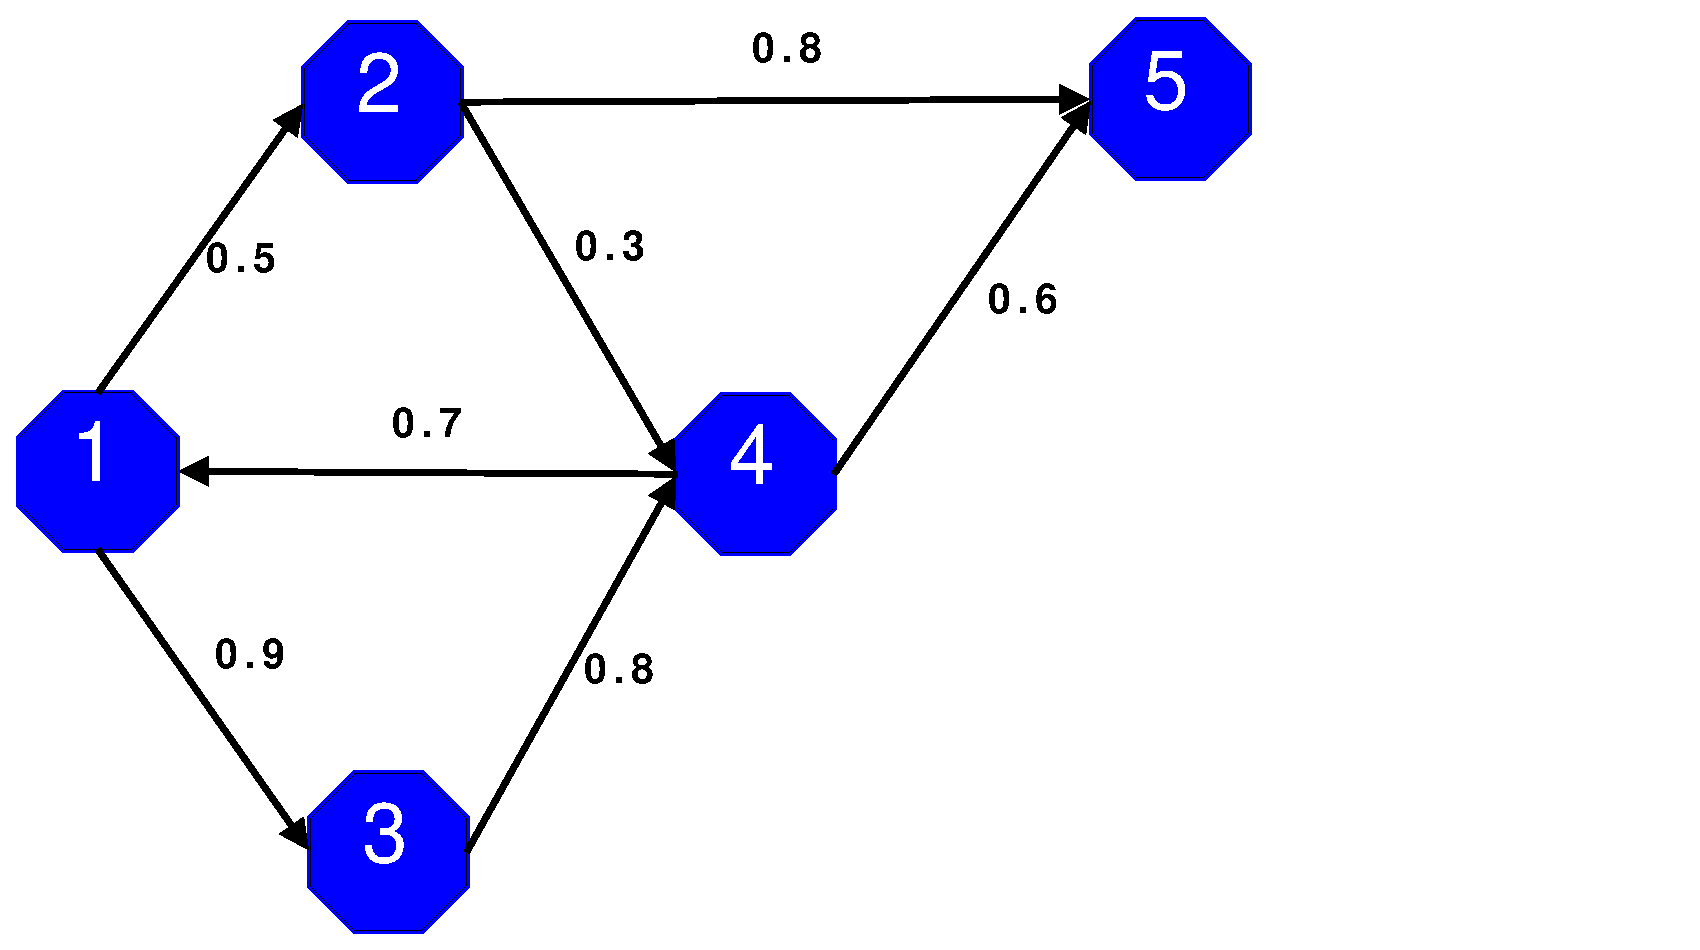
\includegraphics[width=50mm,height=25mm]{../img/graph.eps}
	\end{center}
	\end{figure}

\end{frame}

\begin{frame}[fragile]
	\frametitle{Time-Decaying Facts}
  
  \begin{block}{Why?}
  	The probability of a fact may decrease by time and may not be available after a time period.
  \end{block}
  
  \begin{block}{How?}
	Any monotone decreasing function can be used for diminishing the probability of a fact.
	Sigmoid functions are used in our implementation.
  \end{block}
	
\end{frame}

\begin{frame}[fragile]
	\frametitle{Time-Decaying Facts - Sigmoid Functions}
	\begin{equation}
	\label{sigmoid}
	\nonumber f(x) = 1- \frac{1}{1+e^{\alpha\times(\beta-x)}}
	\end{equation}
	
	\begin{figure}[ht]
	\begin{center}
	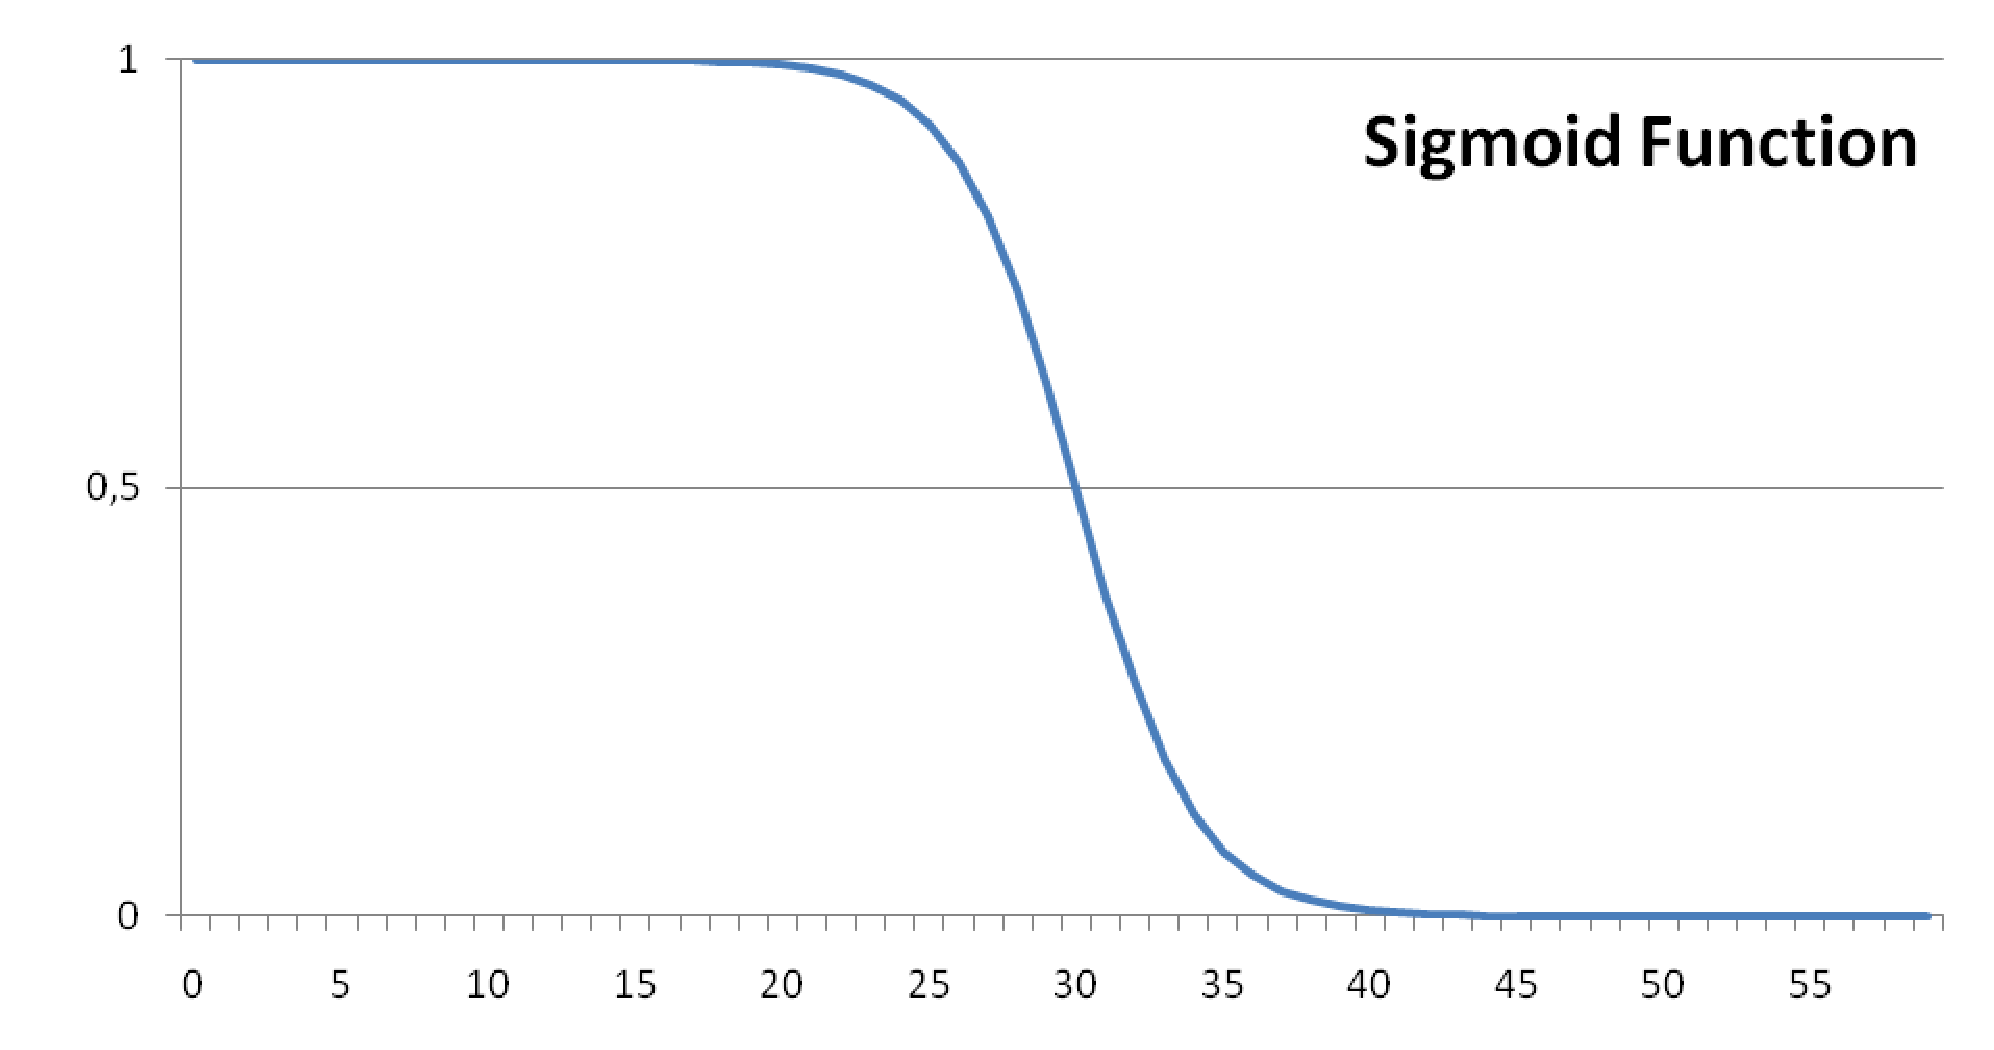
\includegraphics[width=60mm,height=30mm]{../img/sigmoid.eps}
	\caption{Sigmoid function used for time-decaying facts.}
	\label{fig:sigmoid}
	\end{center}
	\end{figure}
	
\end{frame}

\begin{frame}[fragile]
	\frametitle{Time-Decaying Facts - Example}
	\begin{figure}[ht]
	\begin{center}
	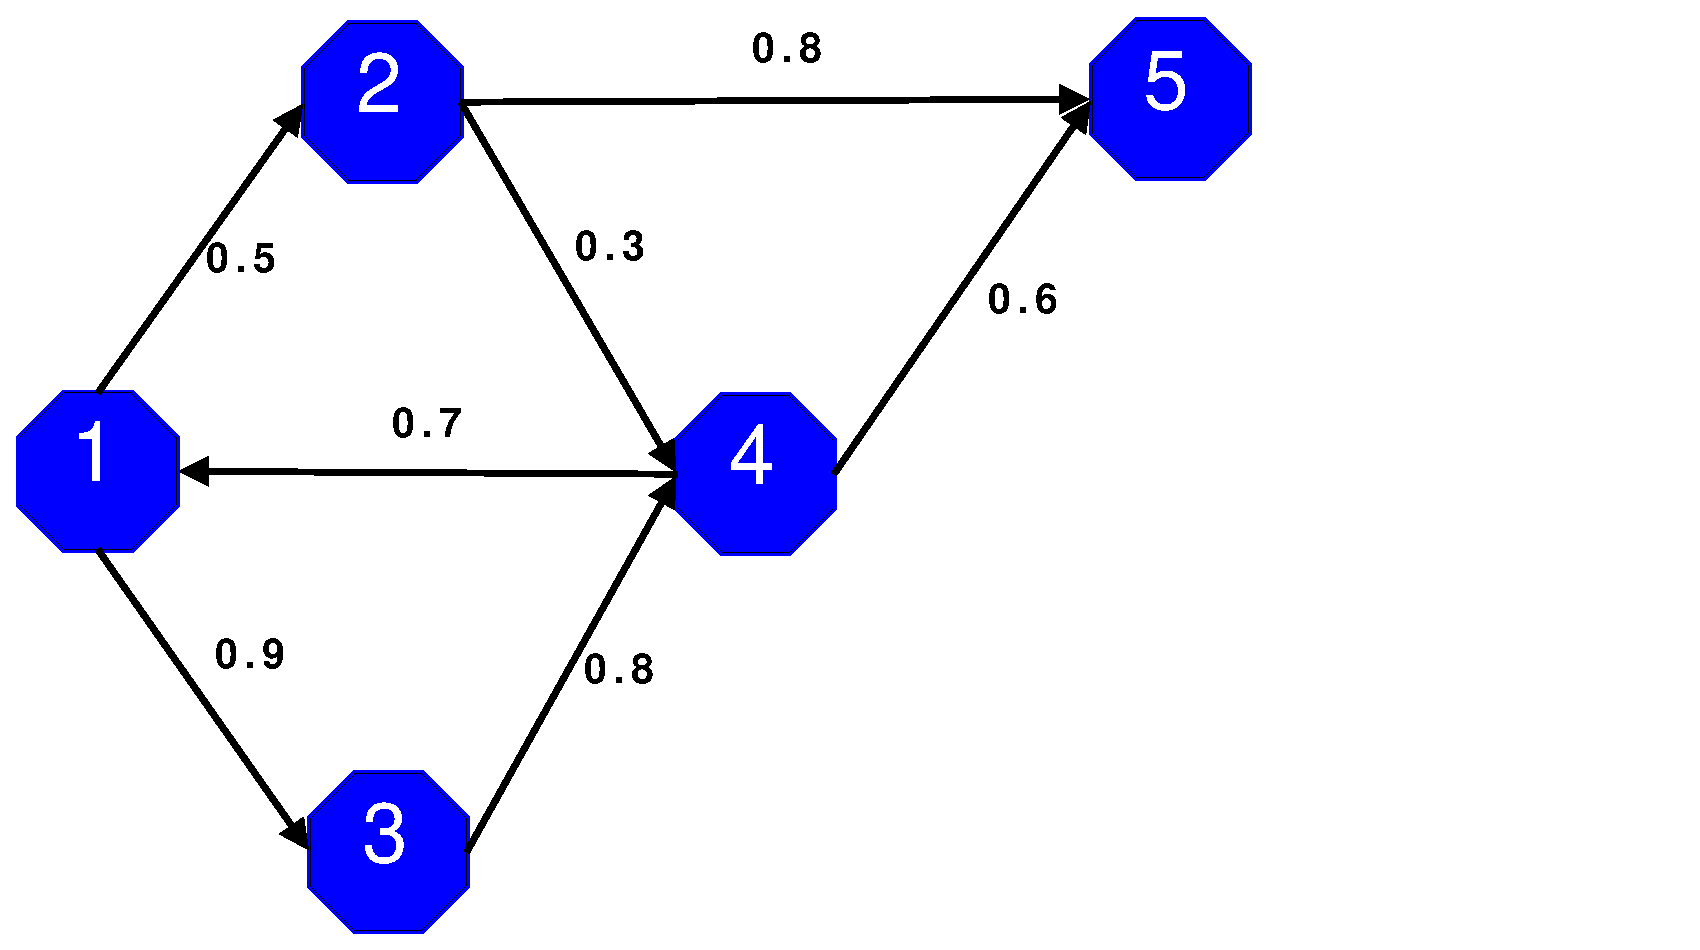
\includegraphics[height=.3\paperheight]{../img/graph.eps}
	\end{center}
	\end{figure}
	\begin{mylisting}
	Rules and Facts
	\vspace*{2px}\hrule
	\begin{verbatim}
	%only replace the fact about edge(2,4)
	%remaining facts and rules are the same...
	"0.3::T::edge(2,4)".
	\end{verbatim}
	\end{mylisting}
	
\end{frame}

\begin{frame}[fragile]
	\frametitle{Time-Decaying Facts - Example (cont'd)}
	\begin{mylisting}
	Query
	\vspace*{2px}\hrule
	\begin{verbatim}
	%initial response to the query
	?- path(2,4,L).
	Prob for this answer:0,299999908226781
	L = [2,4] (0,000 sec) more? (y/n);
	no
	
	%waiting for 30 seconds
	?- path(2,4,L).
	Prob for this answer:0,155176213884928
	L = [2,4] (0,000 sec) more? (y/n)
	no
	
	%after 45 seconds
	?- path(2,4,L).
	no
	\end{verbatim}
	\end{mylisting}
\end{frame}

\frame
{
	\frametitle{Implementation with Belief Networks}
	In the ADES project, 
	\begin{itemize}
		\item The Microsoft Bayesian Network Editor (MSBNx) is used for implementing the BN expert system.
		\item A belief network is created for each regulation by using MSBNx's editor.
		\item These networks are queried at the assertion or retraction of the facts.
	\end{itemize}
}

\frame
{
  \frametitle{Regulation Implementations}
  \begin{table}[!ht]
	\caption{Targeted traffic violations.}
	\centering
	{\tiny
	\begin{tabular}{|r|r|c|}
	\hline
	&&\\
	{\scriptsize No Turn Left} & 
\includegraphics[scale=0.17]{../img/noleft} & {\scriptsize Sign Detection,}\\
	&&\\
	\cline{1-2}
	&&\\
	{\scriptsize No Turn Right} & 
\includegraphics[scale=0.17]{../img/noright} & {\scriptsize RFID Detection,}\\
	&&\\
	\cline{1-2}
	&&\\
	{\scriptsize No U Turn} & 
\includegraphics[scale=0.17]{../img/nouturn} & {\scriptsize GPS/GIS Information,}\\
	&&\\
	\cline{1-2}
	&&\\
	{\scriptsize No Entrance} & 
\includegraphics[scale=0.17]{../img/noenter} & {\scriptsize Vehicle Speed,}\\
	&&\\
	\cline{1-2}
	&&\\
	{\scriptsize Speed Limit} & 
\includegraphics[scale=0.17]{../img/speedlimit} & {\scriptsize Steering Angle,} \\
	&&\\
	\cline{1-2}
	&&\\
	{\scriptsize No Overtaking} & 
\includegraphics[scale=0.17]{../img/overtake} & {\scriptsize Lane Detection,}\\
	&&\\
	\cline{1-2}
	&&\\
	{\scriptsize Traffic Lights} & 
\includegraphics[scale=0.17]{../img/trafficligt} & {\scriptsize Time Elapsed}\\
	&&\\
	\hline
	\end{tabular}  
	}
	\label{viol}
	\end{table}
}

\frame
{
  \frametitle{Regulation Implementations (cont'd)}
	\begin{table}[!ht]
	\caption{Assertion and retraction of the facts.}
	\label{assert}
	{\tiny
	% Table generated by Excel2LaTeX from sheet 'Sayfa1'
	\begin{tabular}{|r|r|r|}
	\hline
	{\bf Regulation} & {\bf Assertion of Facts} & {\bf Retraction of Facts} \\
	\hline
	Directional & Traffic sign detection & After a period of time. \\
	\cline{2-3}
	           & GPS node rule from GIS & Exiting the node. \\
	\cline{2-3}
	           & RFID tag detection (Pre/Post) & After a period of time, \\
	\cline{3-3}
	           &            & Detecting another RFID tag for the same rule. \\
	\hline
	     Speed & Traffic Sign Detection & Restriction ends sign detection, \\
	\cline{3-3}
	           &            & Another speed limit sign. \\
	\cline{2-3}
	           & RFID tag detection & After detecting another RFID tag for the same rule. \\
	\cline{2-3}
	           & GPS node rule from GIS & Exiting the node. \\
	\hline
	Traffic Lights & GPS node rule from GIS & Exiting the node. \\
	\cline{2-3}
	           & RFID tag detection (Pre/Post) & Detecting another RFID tag for the same rule. \\
	\hline
	Illegal Overtake & Traffic sign detection & Restriction ends sign detection. \\
	\cline{2-3}
	           & GPS node rule from GIS & Exiting the node. \\
	\cline{2-3}
	           & Solid Lane Departure & Immediately after query. \\
	\hline
	
	\end{tabular}  
	}
	\end{table}
}

\begin{frame}[fragile]
	\frametitle{Violation of Directional Regulations}
	\begin{figure}[ht]
	\begin{center}
	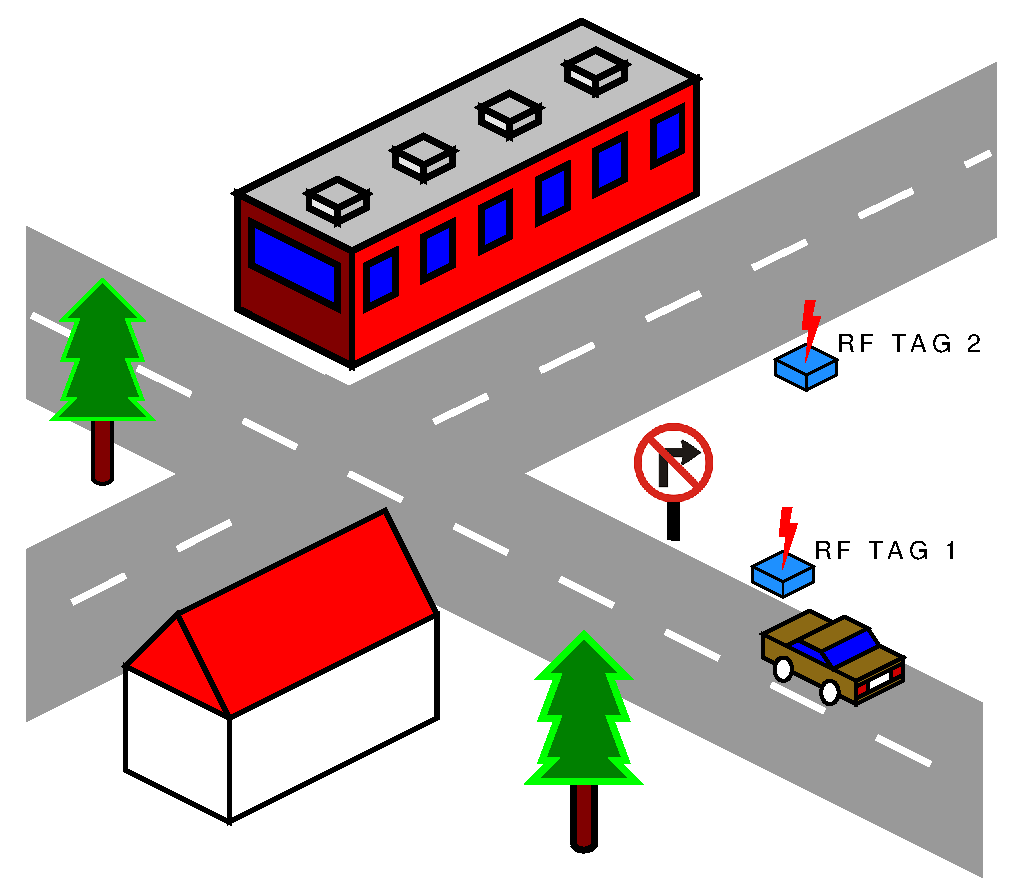
\includegraphics[width=.5\paperwidth]{../img/rfid2.eps}
	\caption{Sample scenario for detecting directional regulation violations.}
	\label{fig:dirreg}
	\end{center}
	\end{figure}
\end{frame}

\begin{frame}[fragile]
	\frametitle{Violation of Directional Regulations (cont'd)}
	\begin{mylisting}
	Rules
	\vspace*{2px}\hrule
	\begin{verbatim}
	%rule declaration
	violation(V,A,P) :- sign_detected(V),
	                    rfid_detected(pre,V),
	                    rfid_detected(post,V), 
	                    gps_node_property(post,V), 
	                    gps_node_property(pre,V), 
	                    A is "N/A",
	                    prob(P),
	                    P>0.8.
	\end{verbatim}
	
	Query
	\vspace*{2px}\hrule
	\begin{verbatim}
	
	Exec: assert("0.9999::T::sign_detected(no_turn_left)").
	Exec: assert("1::T::rfid_detected(pre,no_turn_left)").
	Exec: assert("0.9110::T::gps_node_property(pre,no_turn_left)").
	Exec: assert("0.8962::T::gps_node_property(post,no_turn_left)").
	Exec: assert("1::T::rfid_detected(post,no_turn_left)").
	Exec: violation(V,A,P).
	Prob for this answer:0.816324396689487
	P = 0.816324396689487
	V = no_turn_left
	A = "N/A"
	\end{verbatim}
	\end{mylisting}
\end{frame}

\begin{frame}[fragile]
	\frametitle{Violation of Directional Regulations (cont'd)}
	\begin{figure}
	\begin{center}
	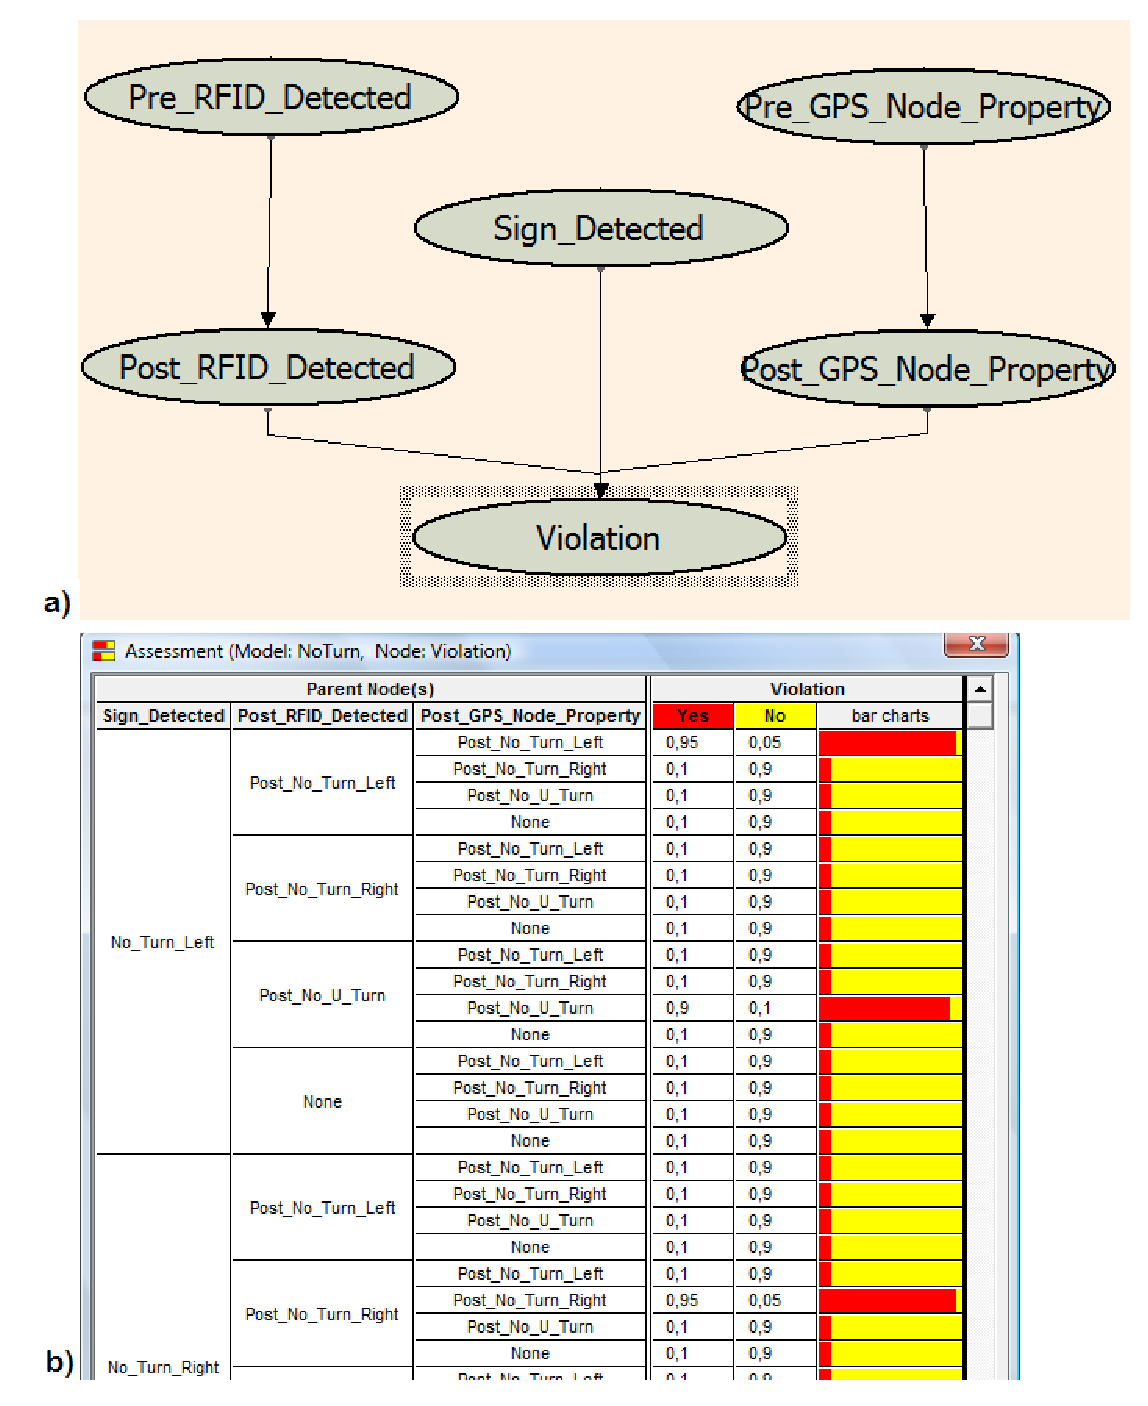
\includegraphics[width=.5\paperwidth]{../img/no_turn_bn.eps}
	\caption{The BN for directional regulations.}
	\label{fig:bnsign}
	\end{center}
	\end{figure}
\end{frame}

\begin{frame}[fragile]
	\frametitle{Violation of Speed Limitation }
	\begin{figure}[ht]
	\begin{center}
	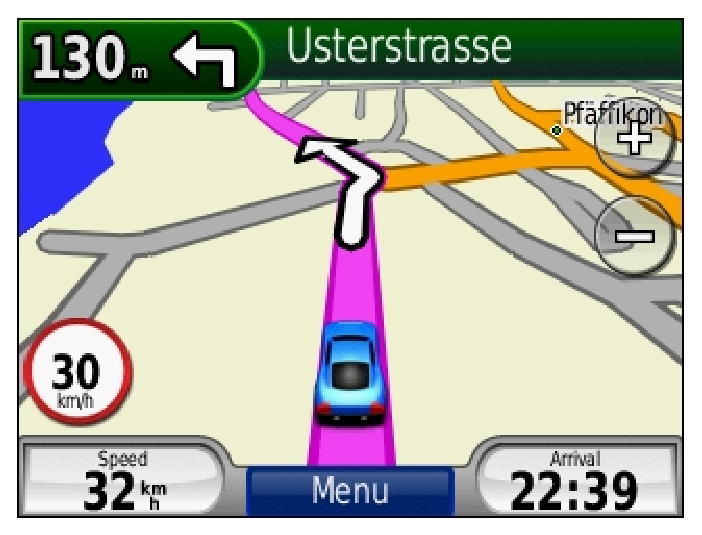
\includegraphics[width=.5\paperwidth]{../img/gpsspeed.eps}
	\caption{Speed limit aware GPS application.}
	\label{fig:gpsspeed}
	\end{center}
	\end{figure}
\end{frame}

\begin{frame}[fragile]
	\frametitle{Violation of Speed Limitation (cont'd)}
	\begin{mylisting}
	Rules
	\vspace*{2px}\hrule
	\begin{verbatim}
	%rule declaration
	violation(V,A,P) :- gps_node_property(V,L),
	                    velocity_exceeds(S),
	                    sign_detected(V,L),
	                    S>=L,
	                    atom_chars(S,L1), append(L1,[95],L2), 
	                    atom_chars(L,L3), append(L2,L3,L4), 
	                    atom_chars(A,L4),
	                    prob(P),
	                    P>0.9.
	\end{verbatim}
	
	Query
	\vspace*{2px}\hrule
	\begin{verbatim}
	
	Exec: assert("1.0000::T::sign_detected(speed_limit,30)").
	Exec: assert("0.9759::T::gps_node_property(speed_limit,30)").
	Exec: assert("1::T::velocity_exceeds(50)").
	Exec: violation(V,A,P).
	Prob for this answer:0.975898794128071
	P = 0.975898794128071
	V = speed_limit
	A = '50_30'
	
	\end{verbatim}
	\end{mylisting}	
\end{frame}

\begin{frame}[fragile]
	\frametitle{Violation of Speed Limitation (cont'd)}
	\begin{figure}[ht]
	\begin{center}
	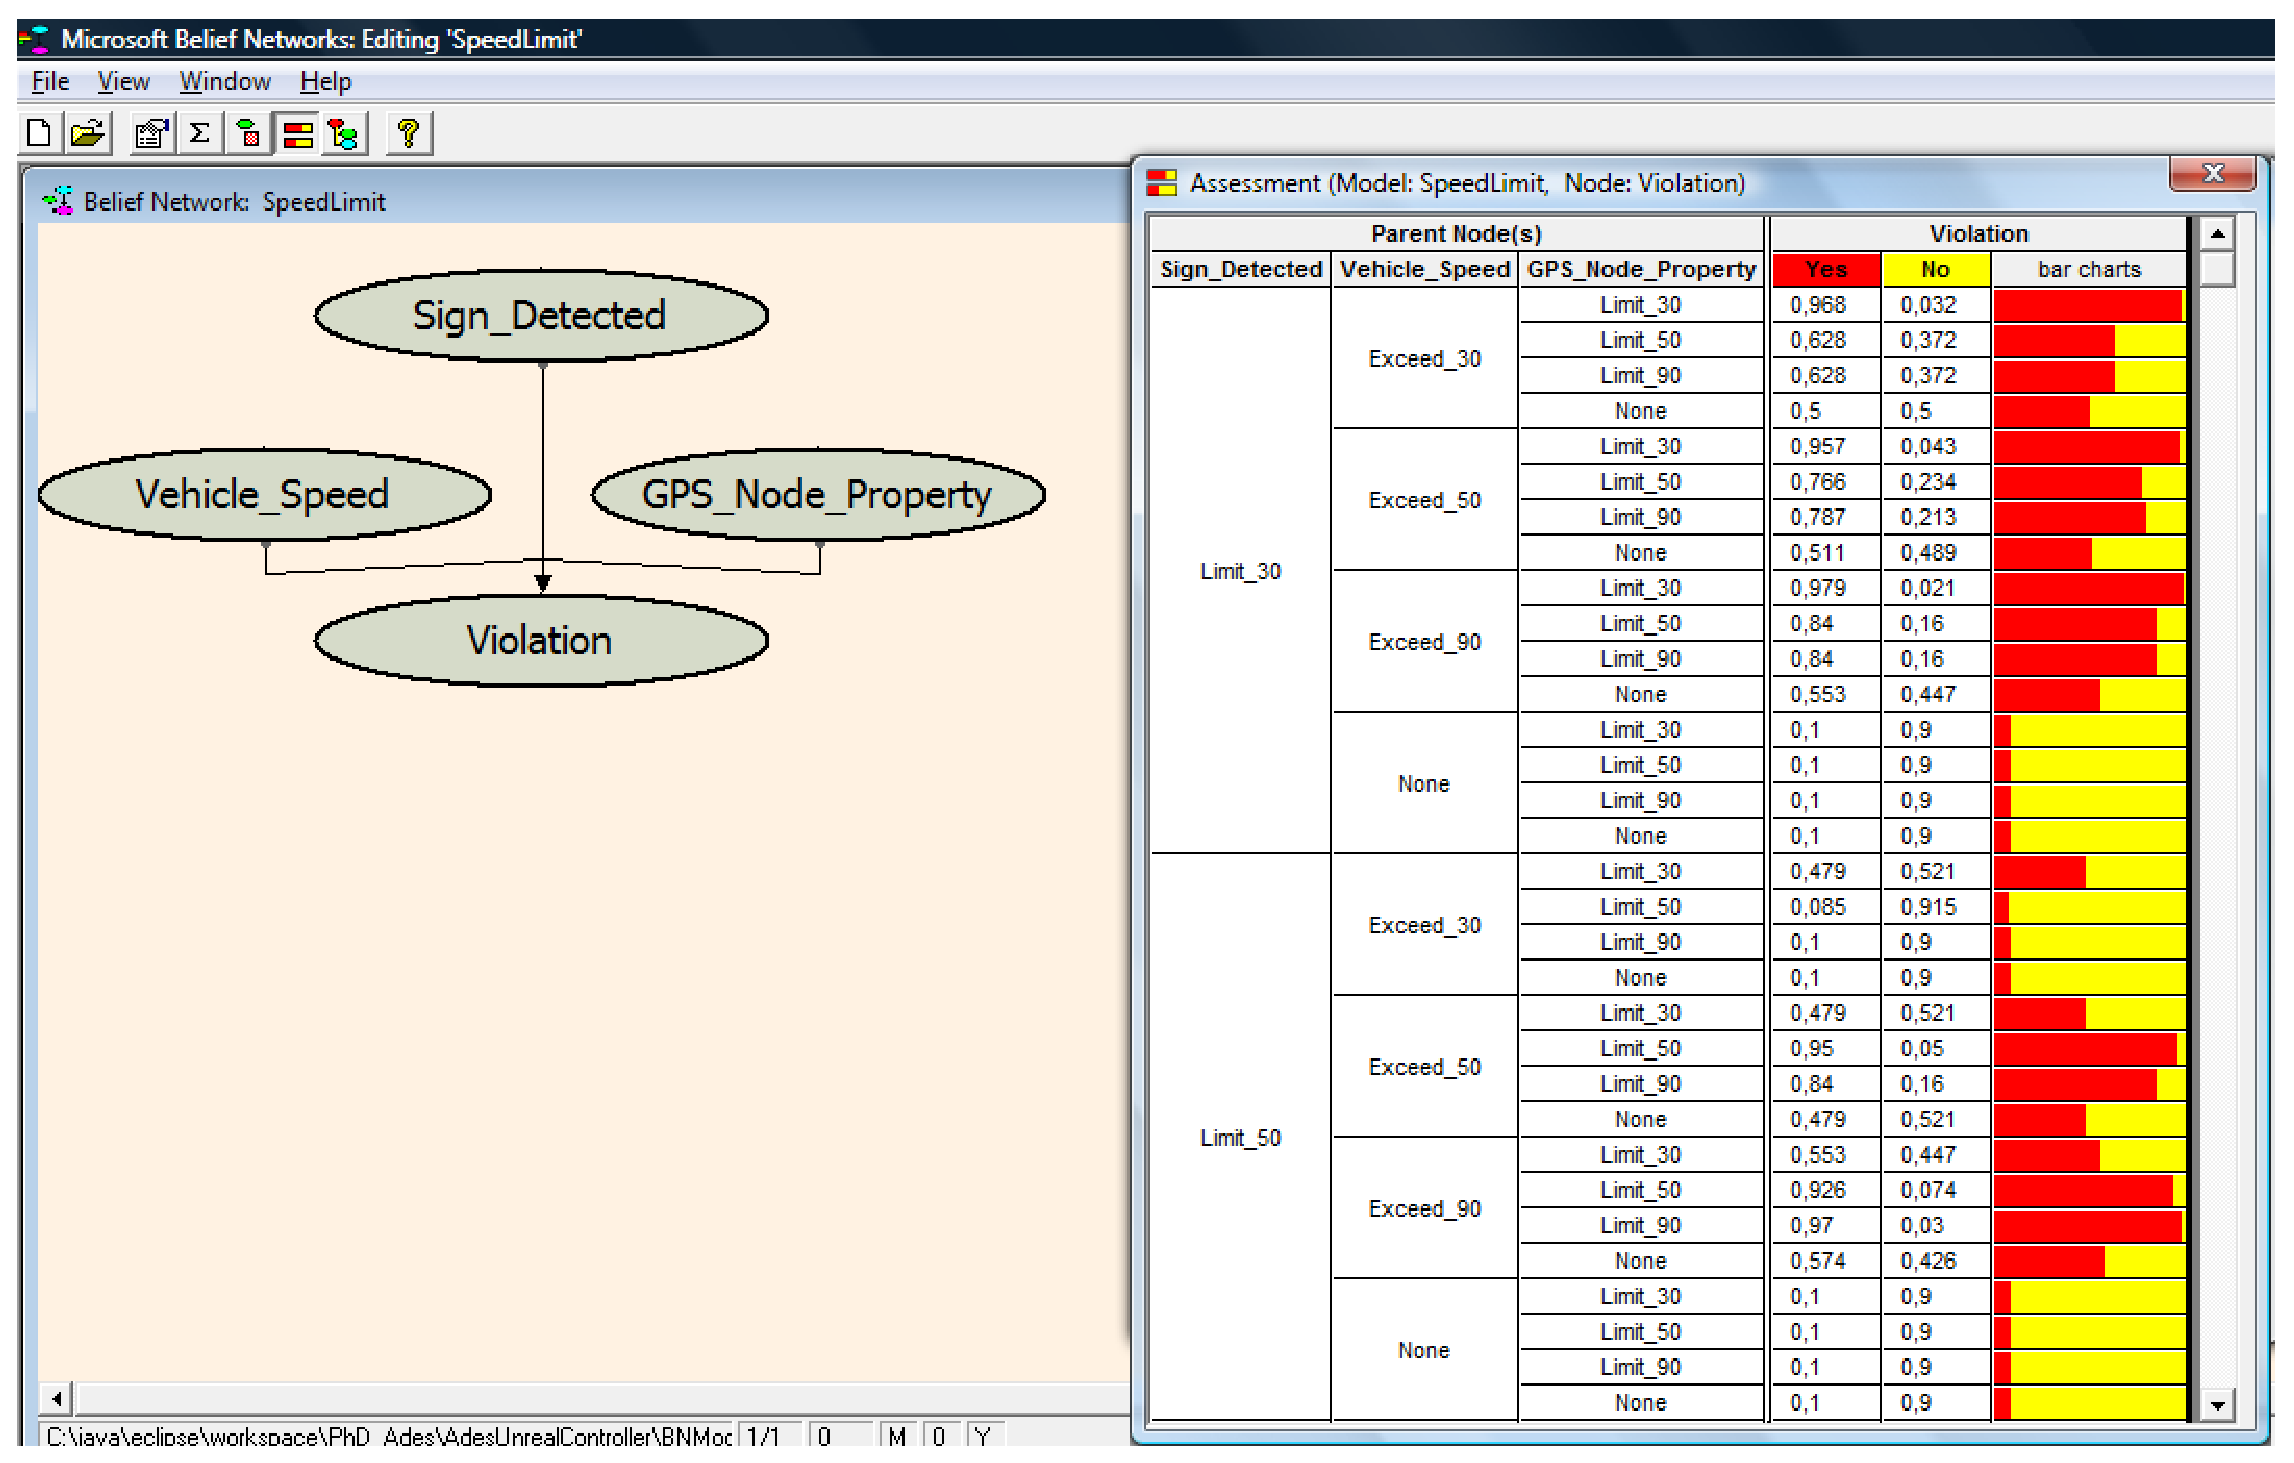
\includegraphics[width=.6\paperwidth]{../img/speed_bn.eps}
	\caption{The belief network and it's property assessments for speed limitations.}
	\label{fig:bnspeed}
	\end{center}
	\end{figure}
\end{frame}


\begin{frame}[fragile]
	\frametitle{Illegal Overtaking}
	\begin{figure}[ht]
	\begin{center}
	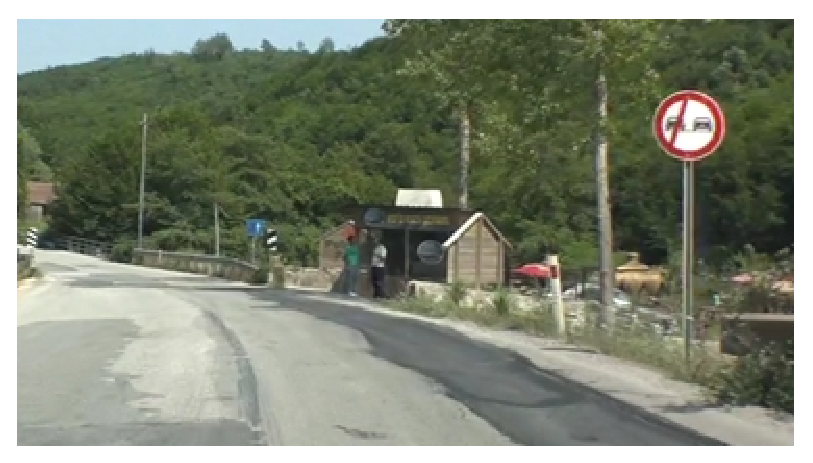
\includegraphics[width=.5\paperwidth]{../img/otfb.eps}
	\caption{Overtake forbidden sign.}
	\label{fig:otfb}
	\end{center}
	\end{figure}	
\end{frame}

\begin{frame}[fragile]
	\frametitle{Illegal Overtaking (cont'd)}
	\begin{mylisting}
	Rules
	\vspace*{2px}\hrule
	\begin{verbatim}
	%rule declaration
	violation(V,A,P) :- sign_detected(no_overtake),
	                    rfid_detected(no_overtake),
	                    gps_node_property(no_overtake),
	                    lane_departure(left),
	                    A is "N/A",
	                    V is "no_overtake",
	                    prob(P).
	\end{verbatim}
	\end{mylisting}	
\end{frame}

\begin{frame}[fragile]
	\frametitle{Illegal Overtaking (cont'd)}
	\begin{figure}[ht]
	\begin{center}
	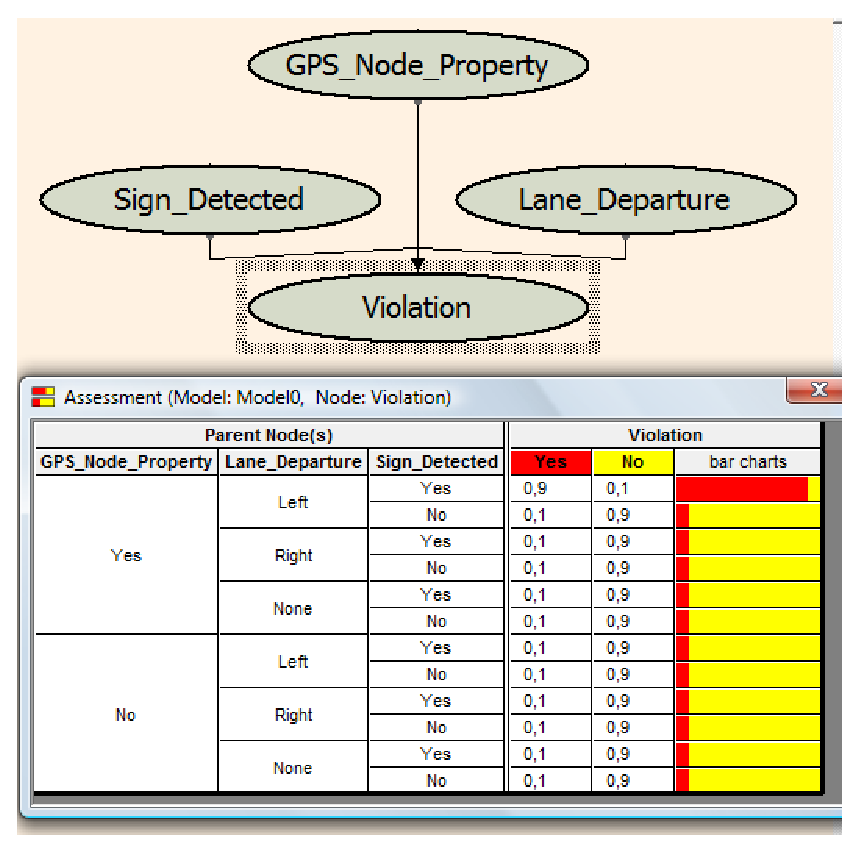
\includegraphics[width=.5\paperwidth]{../img/overtake_bn.eps}
	\caption{The belief network and it's property assessments for illegal overtaking.}
	\label{fig:bnillegal}
	\end{center}
	\end{figure}	
\end{frame}

\begin{frame}[fragile]
	\frametitle{Violation of Red Traffic Lights}
	Active RF tags are required!
	\begin{figure}[ht]
	\begin{center}
	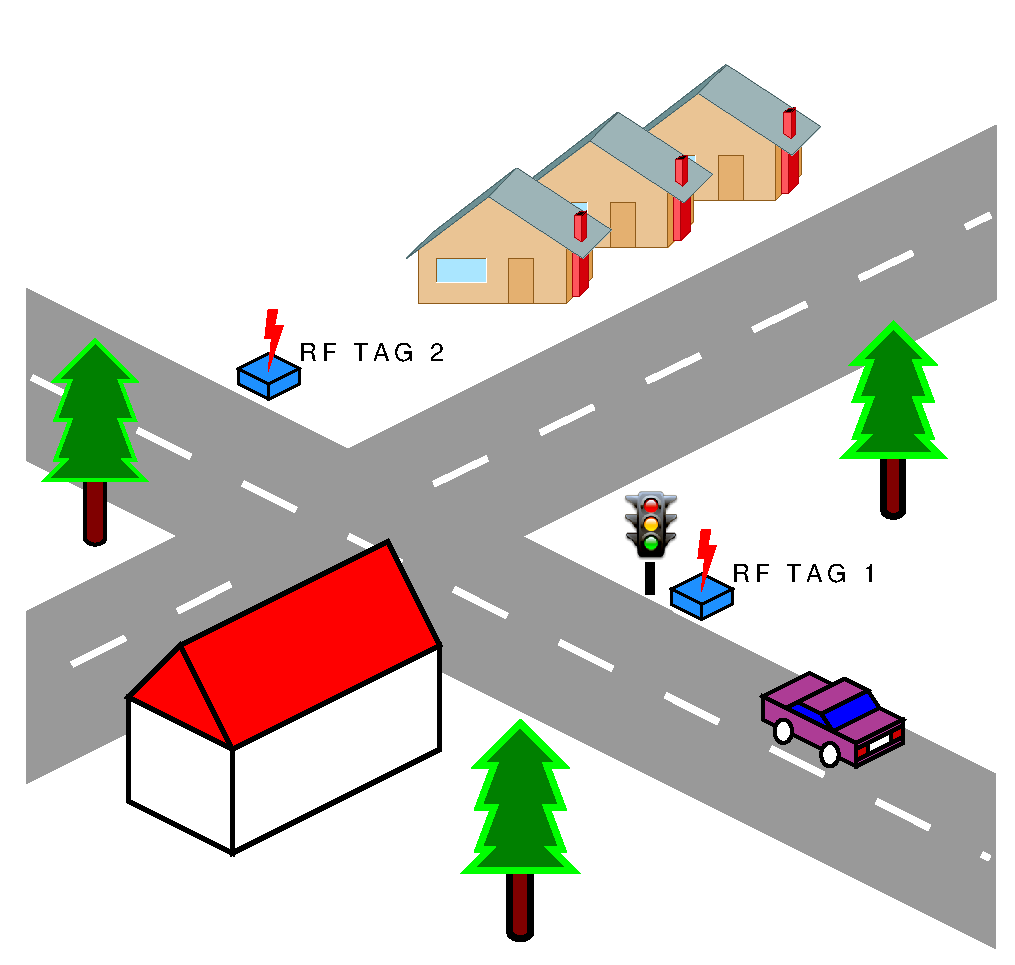
\includegraphics[width=.5\paperwidth]{../img/rfid3.eps}
	\caption{Sample scenario for red light violations.}
	\label{fig:rfid3}
	\end{center}
	\end{figure}
\end{frame}

\begin{frame}[fragile]
	\frametitle{Violation of Red Traffic Lights (cont'd)}
	\begin{mylisting}
	Rules
	\vspace*{2px}\hrule	
	\begin{verbatim}
	%rule declaration
	violation(V,A,P) :- rfid_detected(pre,light_red),
	                    rfid_detected(post,light_red),
	                    gps_node_property(traffic_lights),
	                    A is "N/A",
	                    V is "red_light",
	                    prob(P).
	\end{verbatim}
	\end{mylisting}	
\end{frame}

\begin{frame}[fragile]
	\frametitle{Violation of Red Traffic Lights (cont'd)}
	\begin{figure}[ht]
	\begin{center}
	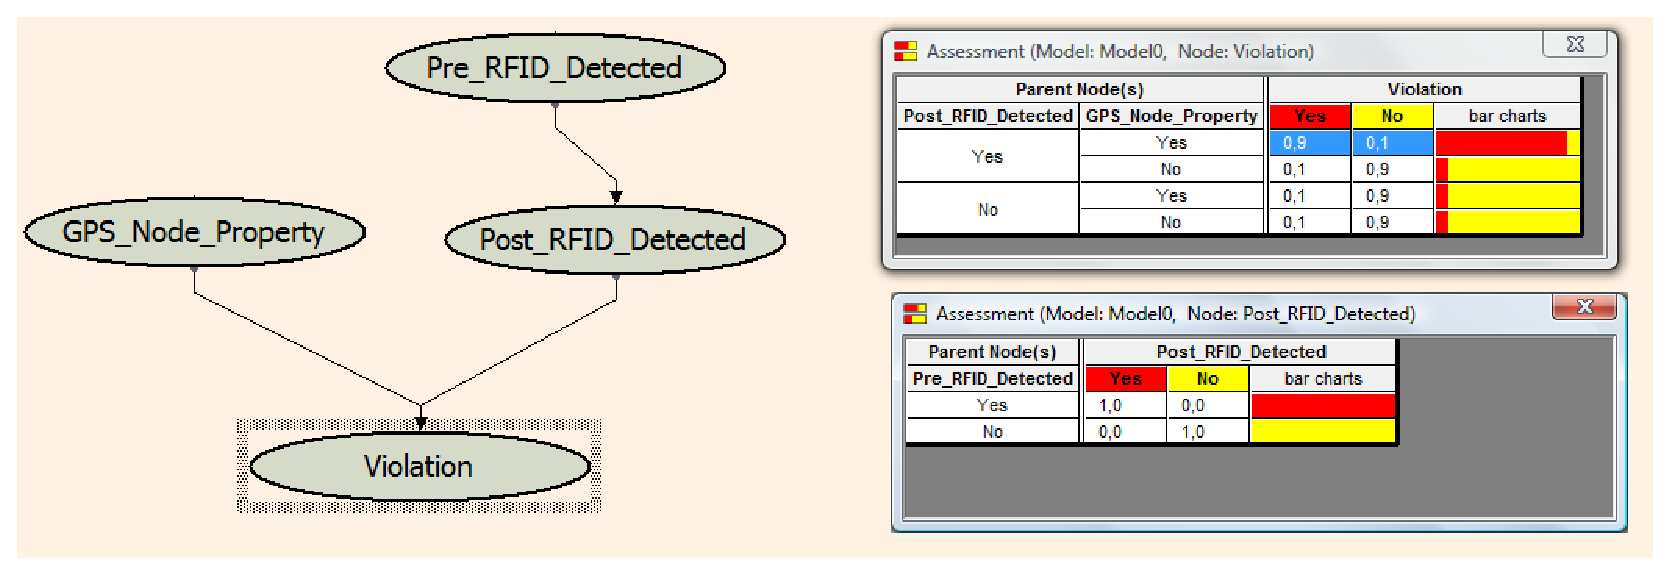
\includegraphics[width=.8\paperwidth]{../img/redlight_bn.eps}
	\caption{The belief network and it's property assessments for traffic light regulations.}
	\label{fig:bnredlight}
	\end{center}
	\end{figure}
\end{frame}

\subsection{Modeling Driver Aggressiveness}
\frame
{
  \frametitle{Modeling Driver Aggressiveness}
  {\small
  \begin{eqnarray}
	\label{eq12}
	Violation &=& \left\{\begin{array}{l} Yes \rightarrow p>t\times(1-\alpha{\times}c/c_{max}), 0<\alpha<1 \\ No \rightarrow o/w \end{array}\right\}
	\end{eqnarray}
	}
}

\section{APPLICATIONS}
\mysectionpage{APPLICATIONS}{APPLICATIONS}

\subsection {The ADES Detector}
\frame
{
	\frametitle{The ADES Detector}
	\begin{figure}[ht]
	\begin{center}
	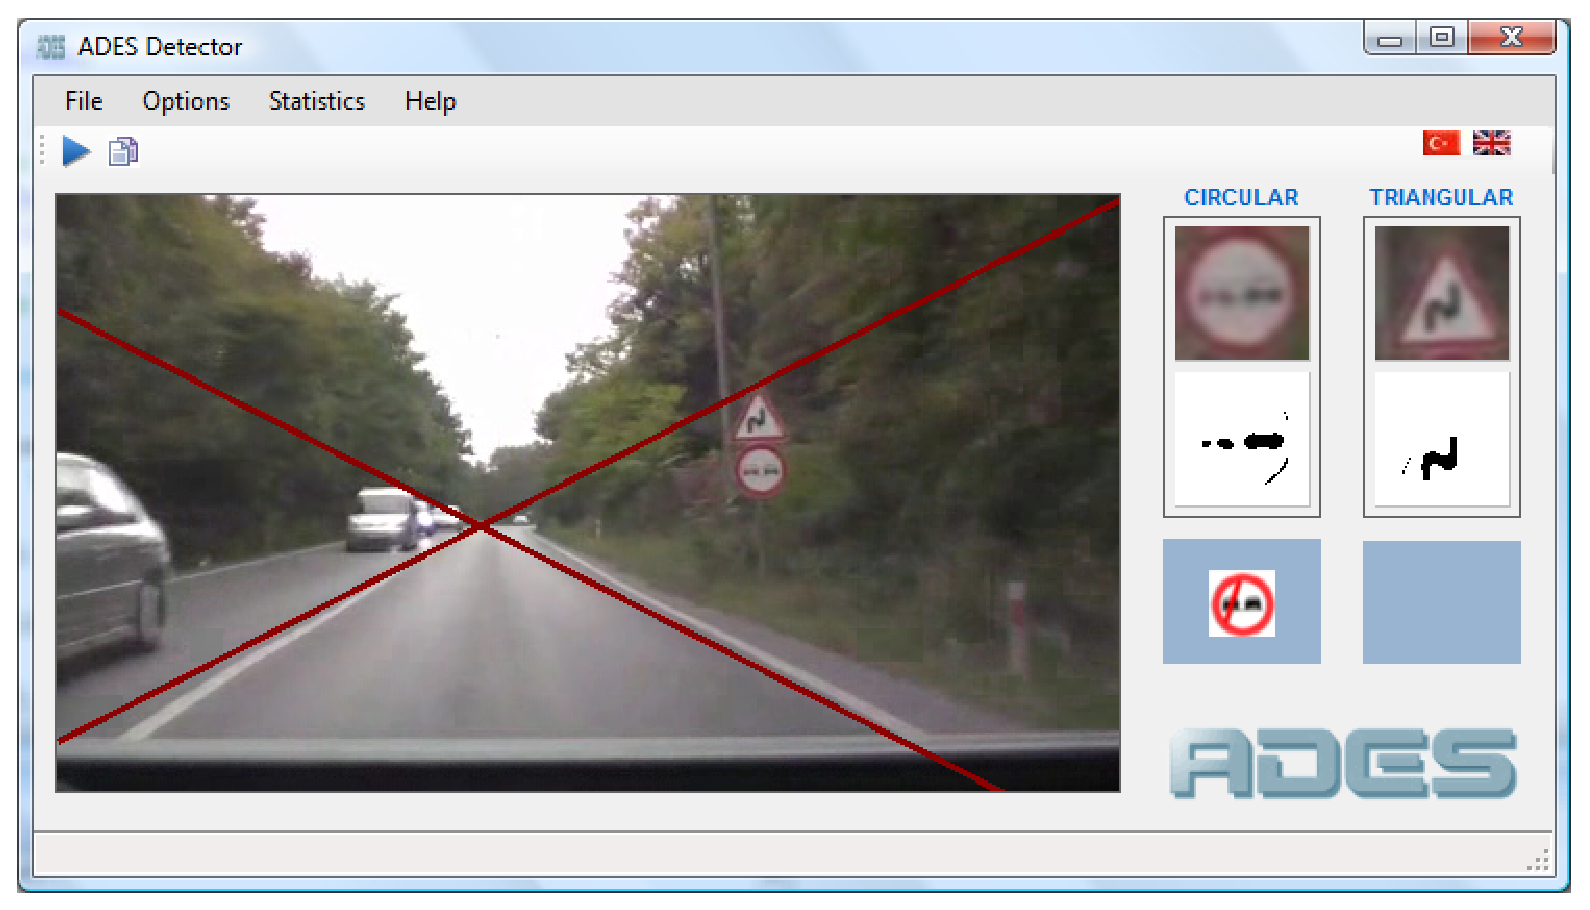
\includegraphics[width=.8\paperwidth]{../img/ADESDetector.eps}
	\caption{The ADES Detector.}
	\label{fig:adesdetector}
	\end{center}
	\end{figure}
}

\subsection{ADES Simulation Environment}
\frame
{
	\frametitle{ADES Simulation Environment}
	\begin{figure}[ht]
	\begin{center}
	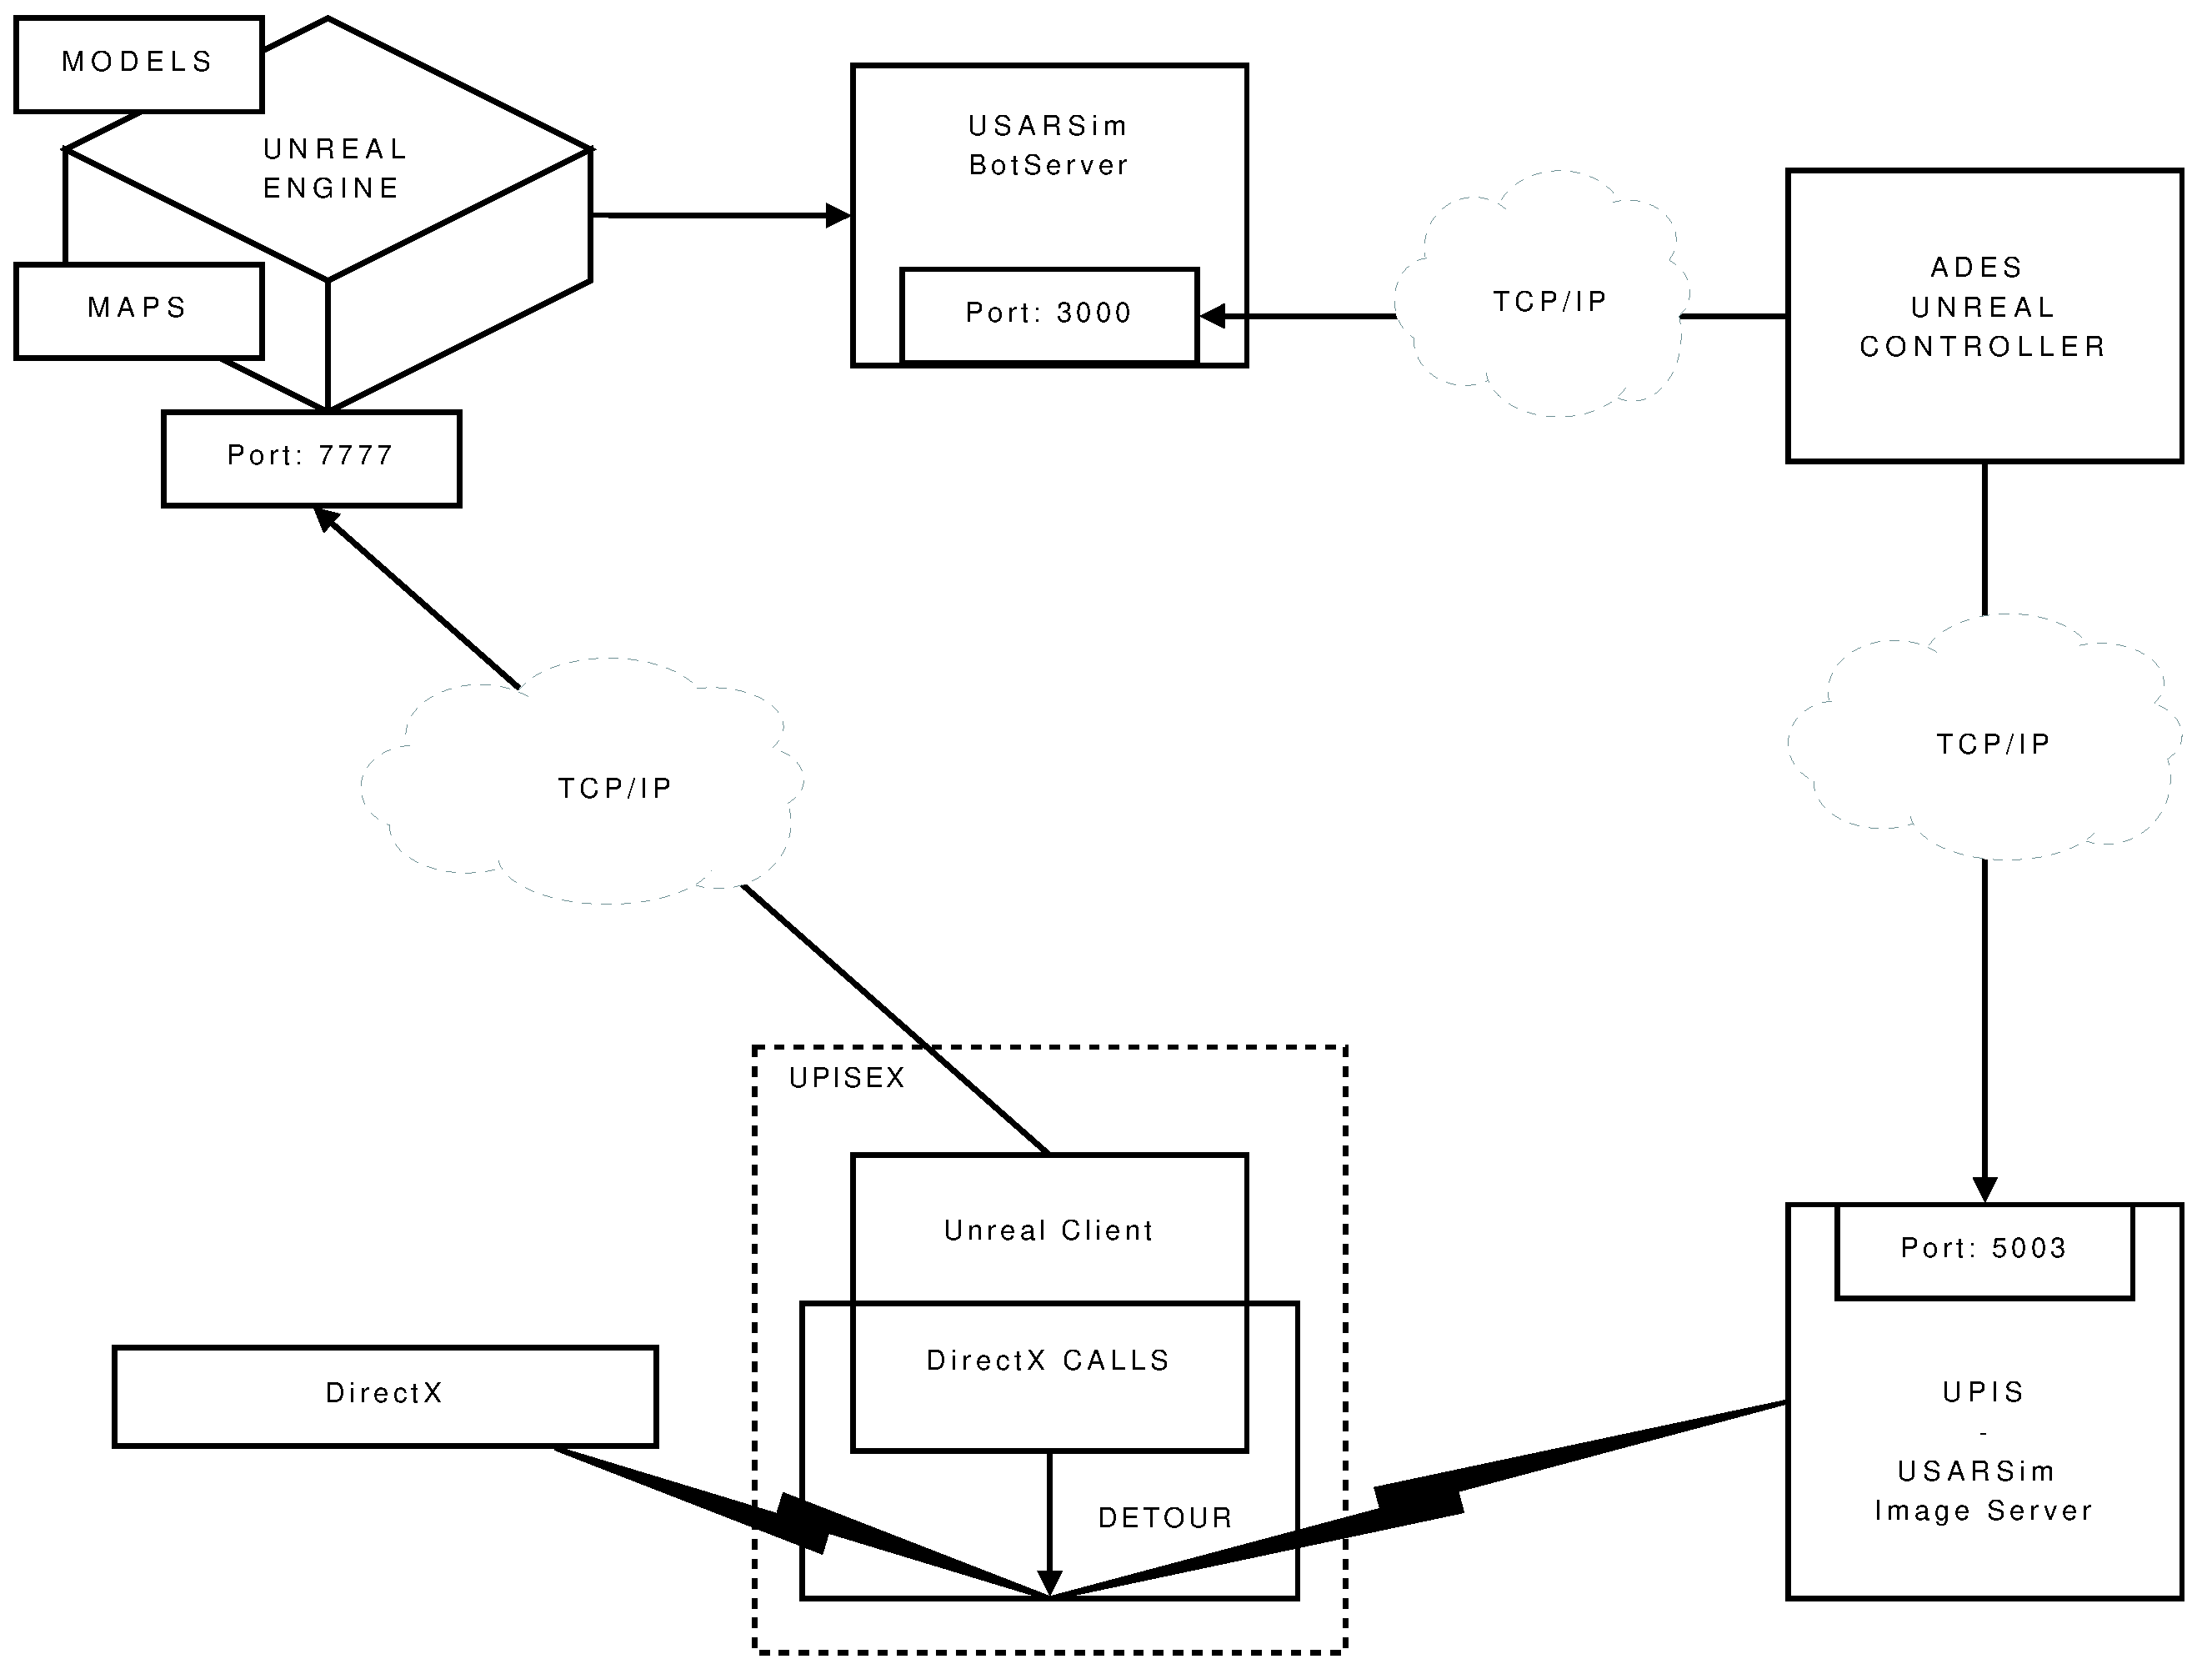
\includegraphics[width=.6\paperwidth]{../img/unrealades.eps}
	\caption{Interaction between Unreal Engine, USARSim and Unreal ADES controller.}
	\label{fig:unrealades}
	\end{center}
	\end{figure}	
}

\frame
{
	\frametitle{Unreal Engine}
	\begin{itemize}
		\item A commercial game engine from Epic Games.
		\item First version UE1 released on 1998. ADES on UE2.5.
		\item Powerful visual rendering and physical modeling.
		\item Provides object oriented programming called the UnrealScript.
	\end{itemize}
}
		
\begin{frame}
	\frametitle{USARSim}
	\begin{block}{}
		USARSim is an Unreal Engine expansion for urban search and rescue (USAR) robots and environments.
	\end{block}
	\begin{itemize}
		\item Open source research tool.
		\item Used in many domains like DARPA and NIST applications. 
		\item RoboCup Rescue Virtual Robots Championship based on USARSim.
		\item Provides numerous models for the use of researchers.
	\end{itemize}
\end{frame}

\begin{frame}
	\frametitle{USARSim - Sedan Class}
	\begin{figure}[ht]
	\begin{center}
	\includegraphics[width=.6\paperwidth]{../img/Sedan.eps}
	\caption{The Sedan in the ADES Unreal world.}
	\label{fig:Sedan}
	\end{center}
	\end{figure}
\end{frame}

\begin{frame}
	\frametitle{USARSim - Sedan Class (cont'd)}
	\begin{table}
	\caption{The class hierarchy of Sedan class.}
	{\tiny
	\begin{center}
	\begin{tabular}{|r|r|r|}
	\hline
	           & \multicolumn{ 2}{|l|}{{\bf Unreal Classes (Commercial)}} \\
	\hline
	           & {\bf Class} & {\bf Description} \\
	\hline
	         1 &      Actor & The base class of every object that have a position in the Unreal world. \\
	\hline
	         2 &       Pawn & Parent class for all controlled entities. \\
	\hline
	         3 &    Vehicle & Parent class for all vehicles controlled by the player. \\
	\hline
	         4 &   KVehicle & Vehicles Karma physics. \\
	\hline
	           & \multicolumn{ 2}{|l|}{{\bf USARSim Classes (Open Source)}} \\
	\hline
	           & {\bf Class} & {\bf Description} \\
	\hline
	         5 &     KRobot & USARSim's physical robot base \\
	\hline
	         6 & GroundVehicle & Vehicles with wheels and steering \\
	\hline
	         7 & AckermanSteeredRobot & Ackerman Steered Vehicles \\
	\hline
	         8 &      Sedan & The Sedan class used by ADES Unreal Controller \\
	\hline
	\end{tabular}
	\end{center}
	}
	\label{tab:sedanclass}
	\end{table}
\end{frame}

\begin{frame}[fragile]
	\frametitle{USARSim - Sedan Class (cont'd)}
	\begin{mylisting}
	From the Usarsim.ini file in UT2004$\backslash$System directory. 
	\vspace*{2pt}\hrule
	{\tiny	
	\begin{verbatim}
	[USARBot.Sedan]
	bDebug=False
	Weight=5
	Payload=2
	ChassisMass=10
	MaxTorque=200.0
	MotorTorque=200.0
	bMountByUU=False
	JointParts=(PartName="RightFWheel",PartClass=class'USARModels.SedanTireRight' ...
	JointParts=(PartName="LeftFWheel",PartClass=class'USARModels.SedanTireLeft',. ..
	JointParts=(PartName="RightRWheel",PartClass=class'USARModels.SedanTireRight', ...
	JointParts=(PartName="LeftRWheel",PartClass=class'USARModels.SedanTireLeft', ...
	MisPkgs=(PkgName="CameraPanTilt",PkgClass=Class'USARMisPkg.CameraPanTilt')...
	Cameras=(ItemClass=class'USARBot.RobotCamera',...
	Sensors=(ItemClass=class'USARBot.GroundTruth', ...
	Sensors=(ItemClass=class'USARBot.RFIDSensor', ...
	Sensors=(ItemClass=class'USARBot.GPSSensor', ...
	\end{verbatim}
	}
	\end{mylisting}
\end{frame}

\begin{frame}
	\frametitle{UnrealEd - The Unreal Level Editor}
	\begin{figure}[ht]
	\begin{center}
	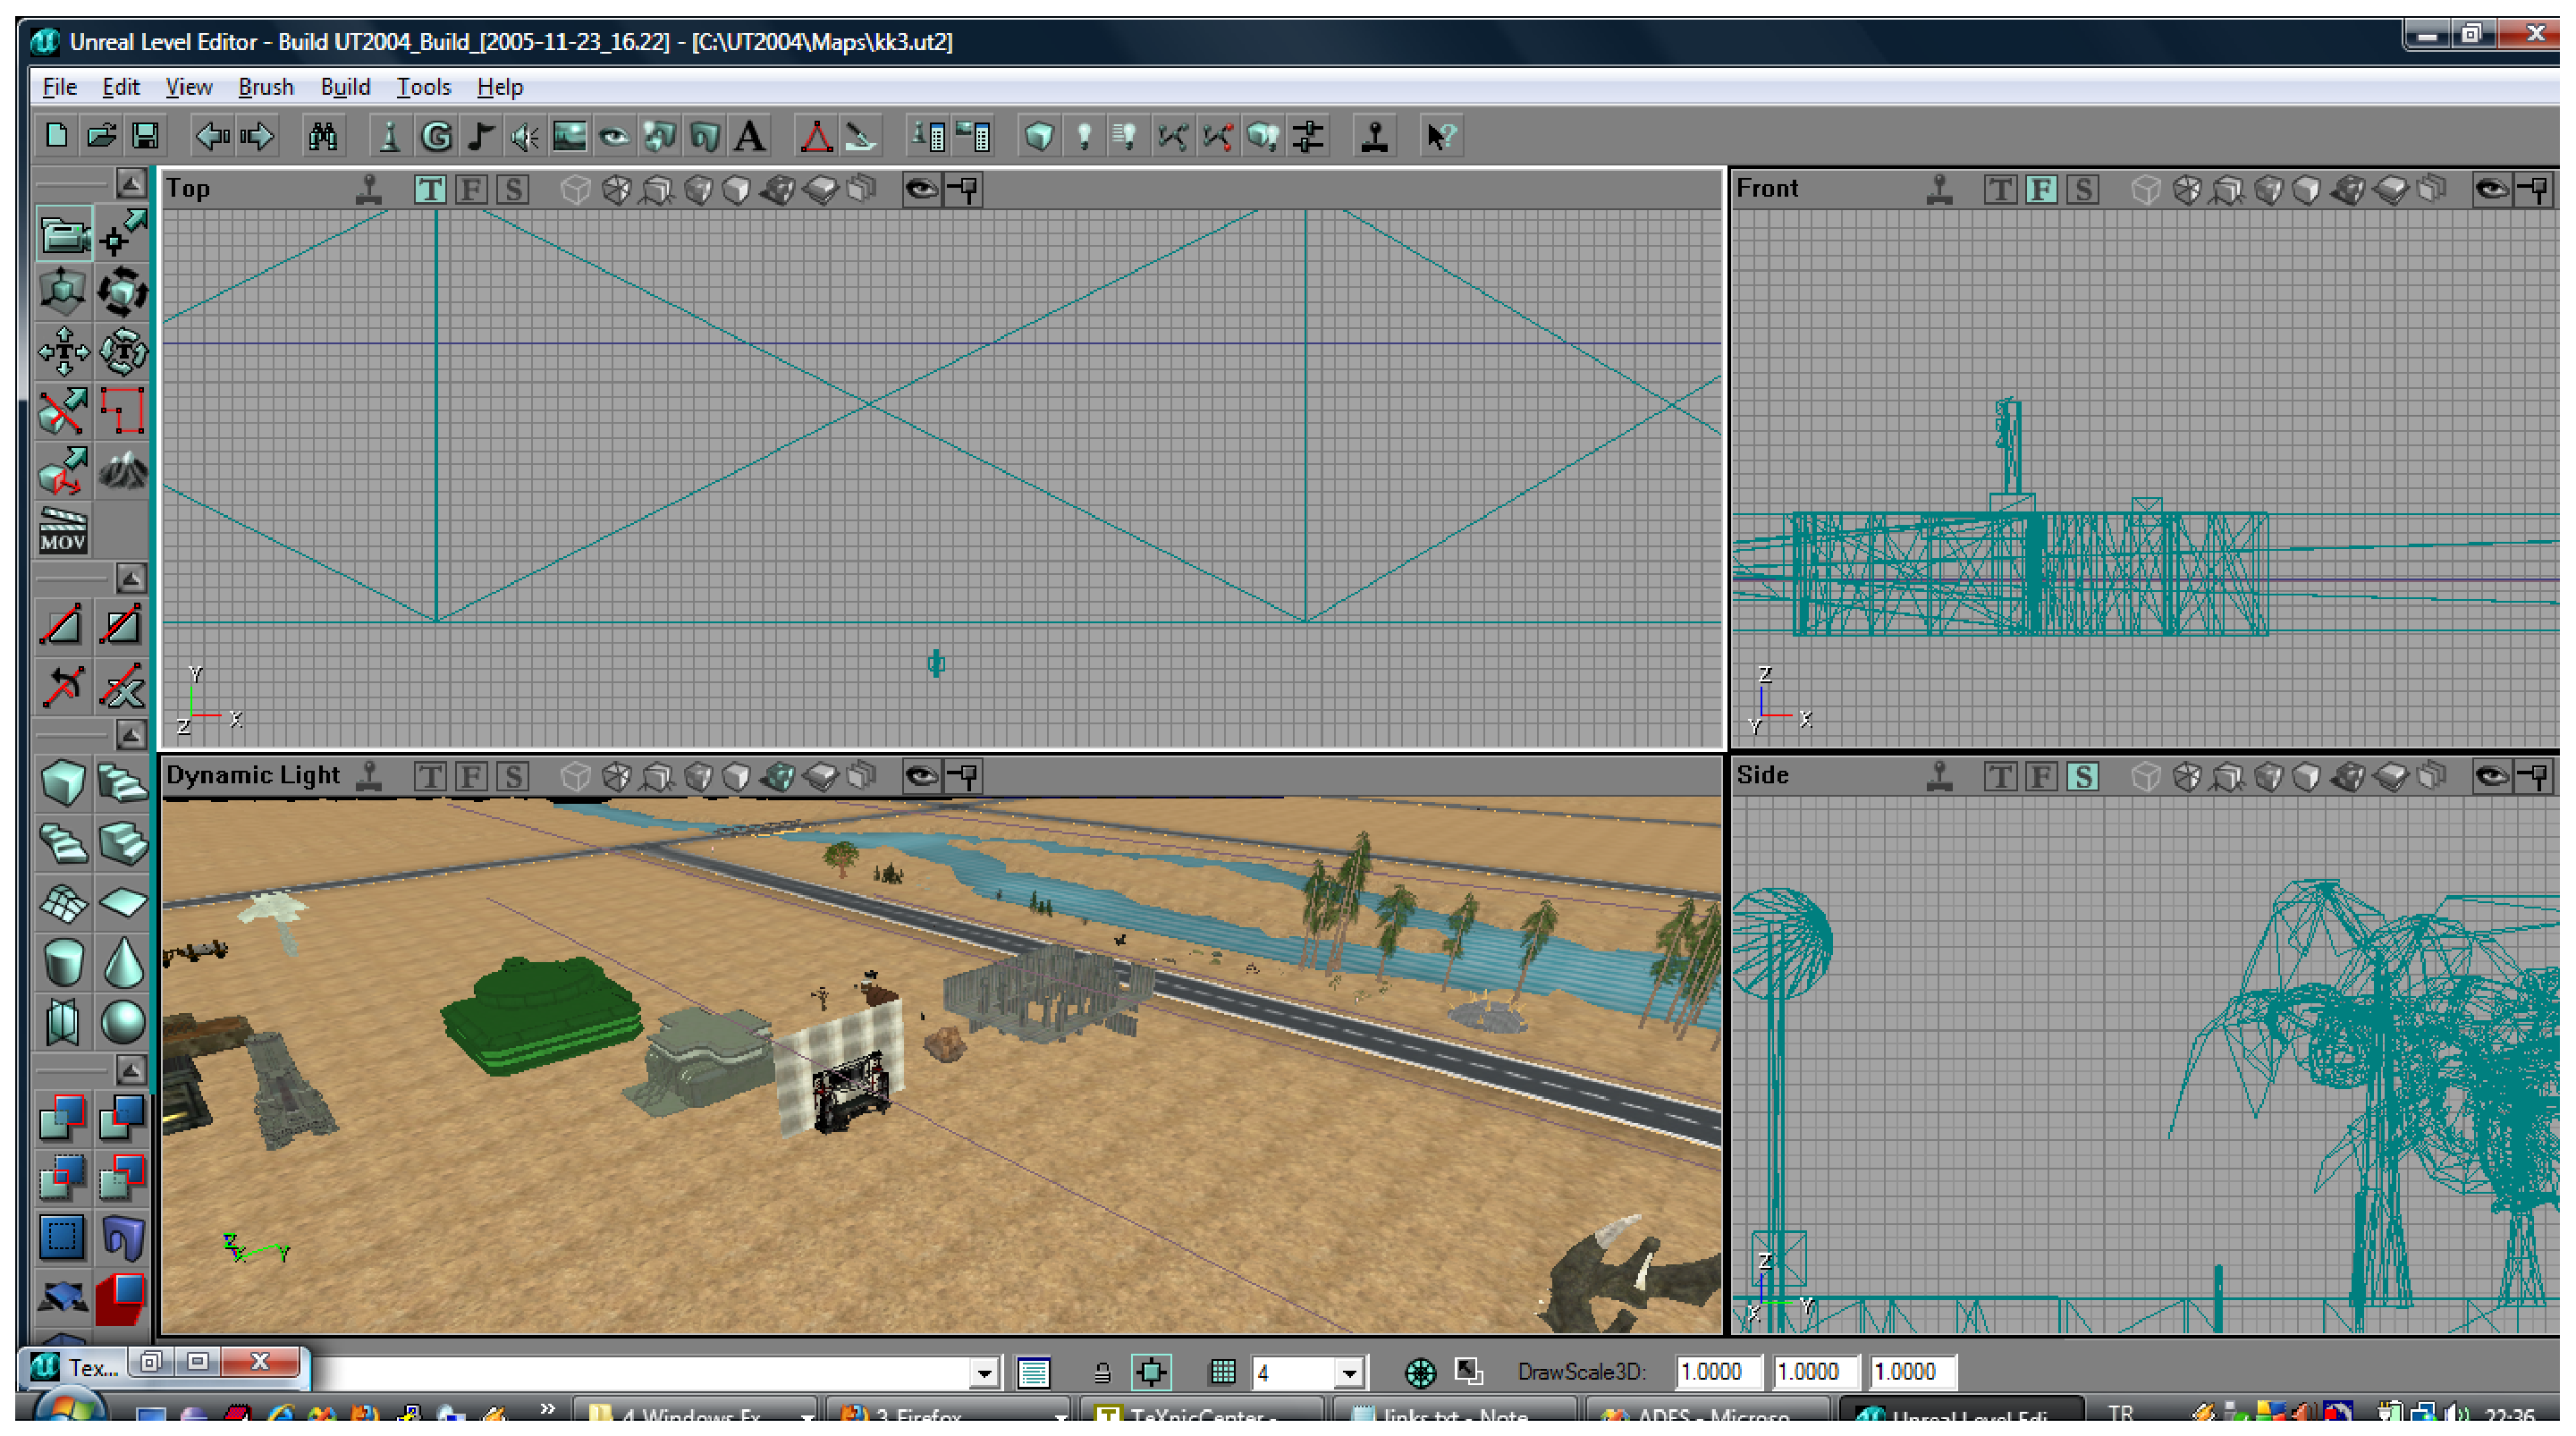
\includegraphics[width=.6\paperwidth]{../img/UnrealEdQuad.eps}
	\caption{The ADES Unreal world in UnrealEd.}
	\label{fig:UnrealEdQuad}
	\end{center}
	\end{figure}
\end{frame}

\begin{frame}
	\frametitle{UnrealEd - Artifacts}
	\begin{itemize}
	    \item \textbf{Actors:} Any object that can be placed into the environment. These objects can be controlled pawns like Sedan, or, other items like pickups, decorations, zone information etc.
	    \item \textbf{Textures:} Textures are images which can be applied to the new created shapes by using brushes.
	    \item \textbf{Static Meshes:} The reusable objects which contain previously created shapes covered with textures.
	    \item \textbf{Meshes and Animations:} Set of meshes which forms repeating animations for shapes.
	    \item \textbf{Other Artifacts:} Sounds, Music, Prefabs (saved brushes).
	\end{itemize}
\end{frame}

\begin{frame}
	\frametitle{UnrealEd - Static Meshes}
	\begin{figure}[ht]
	\begin{center}
	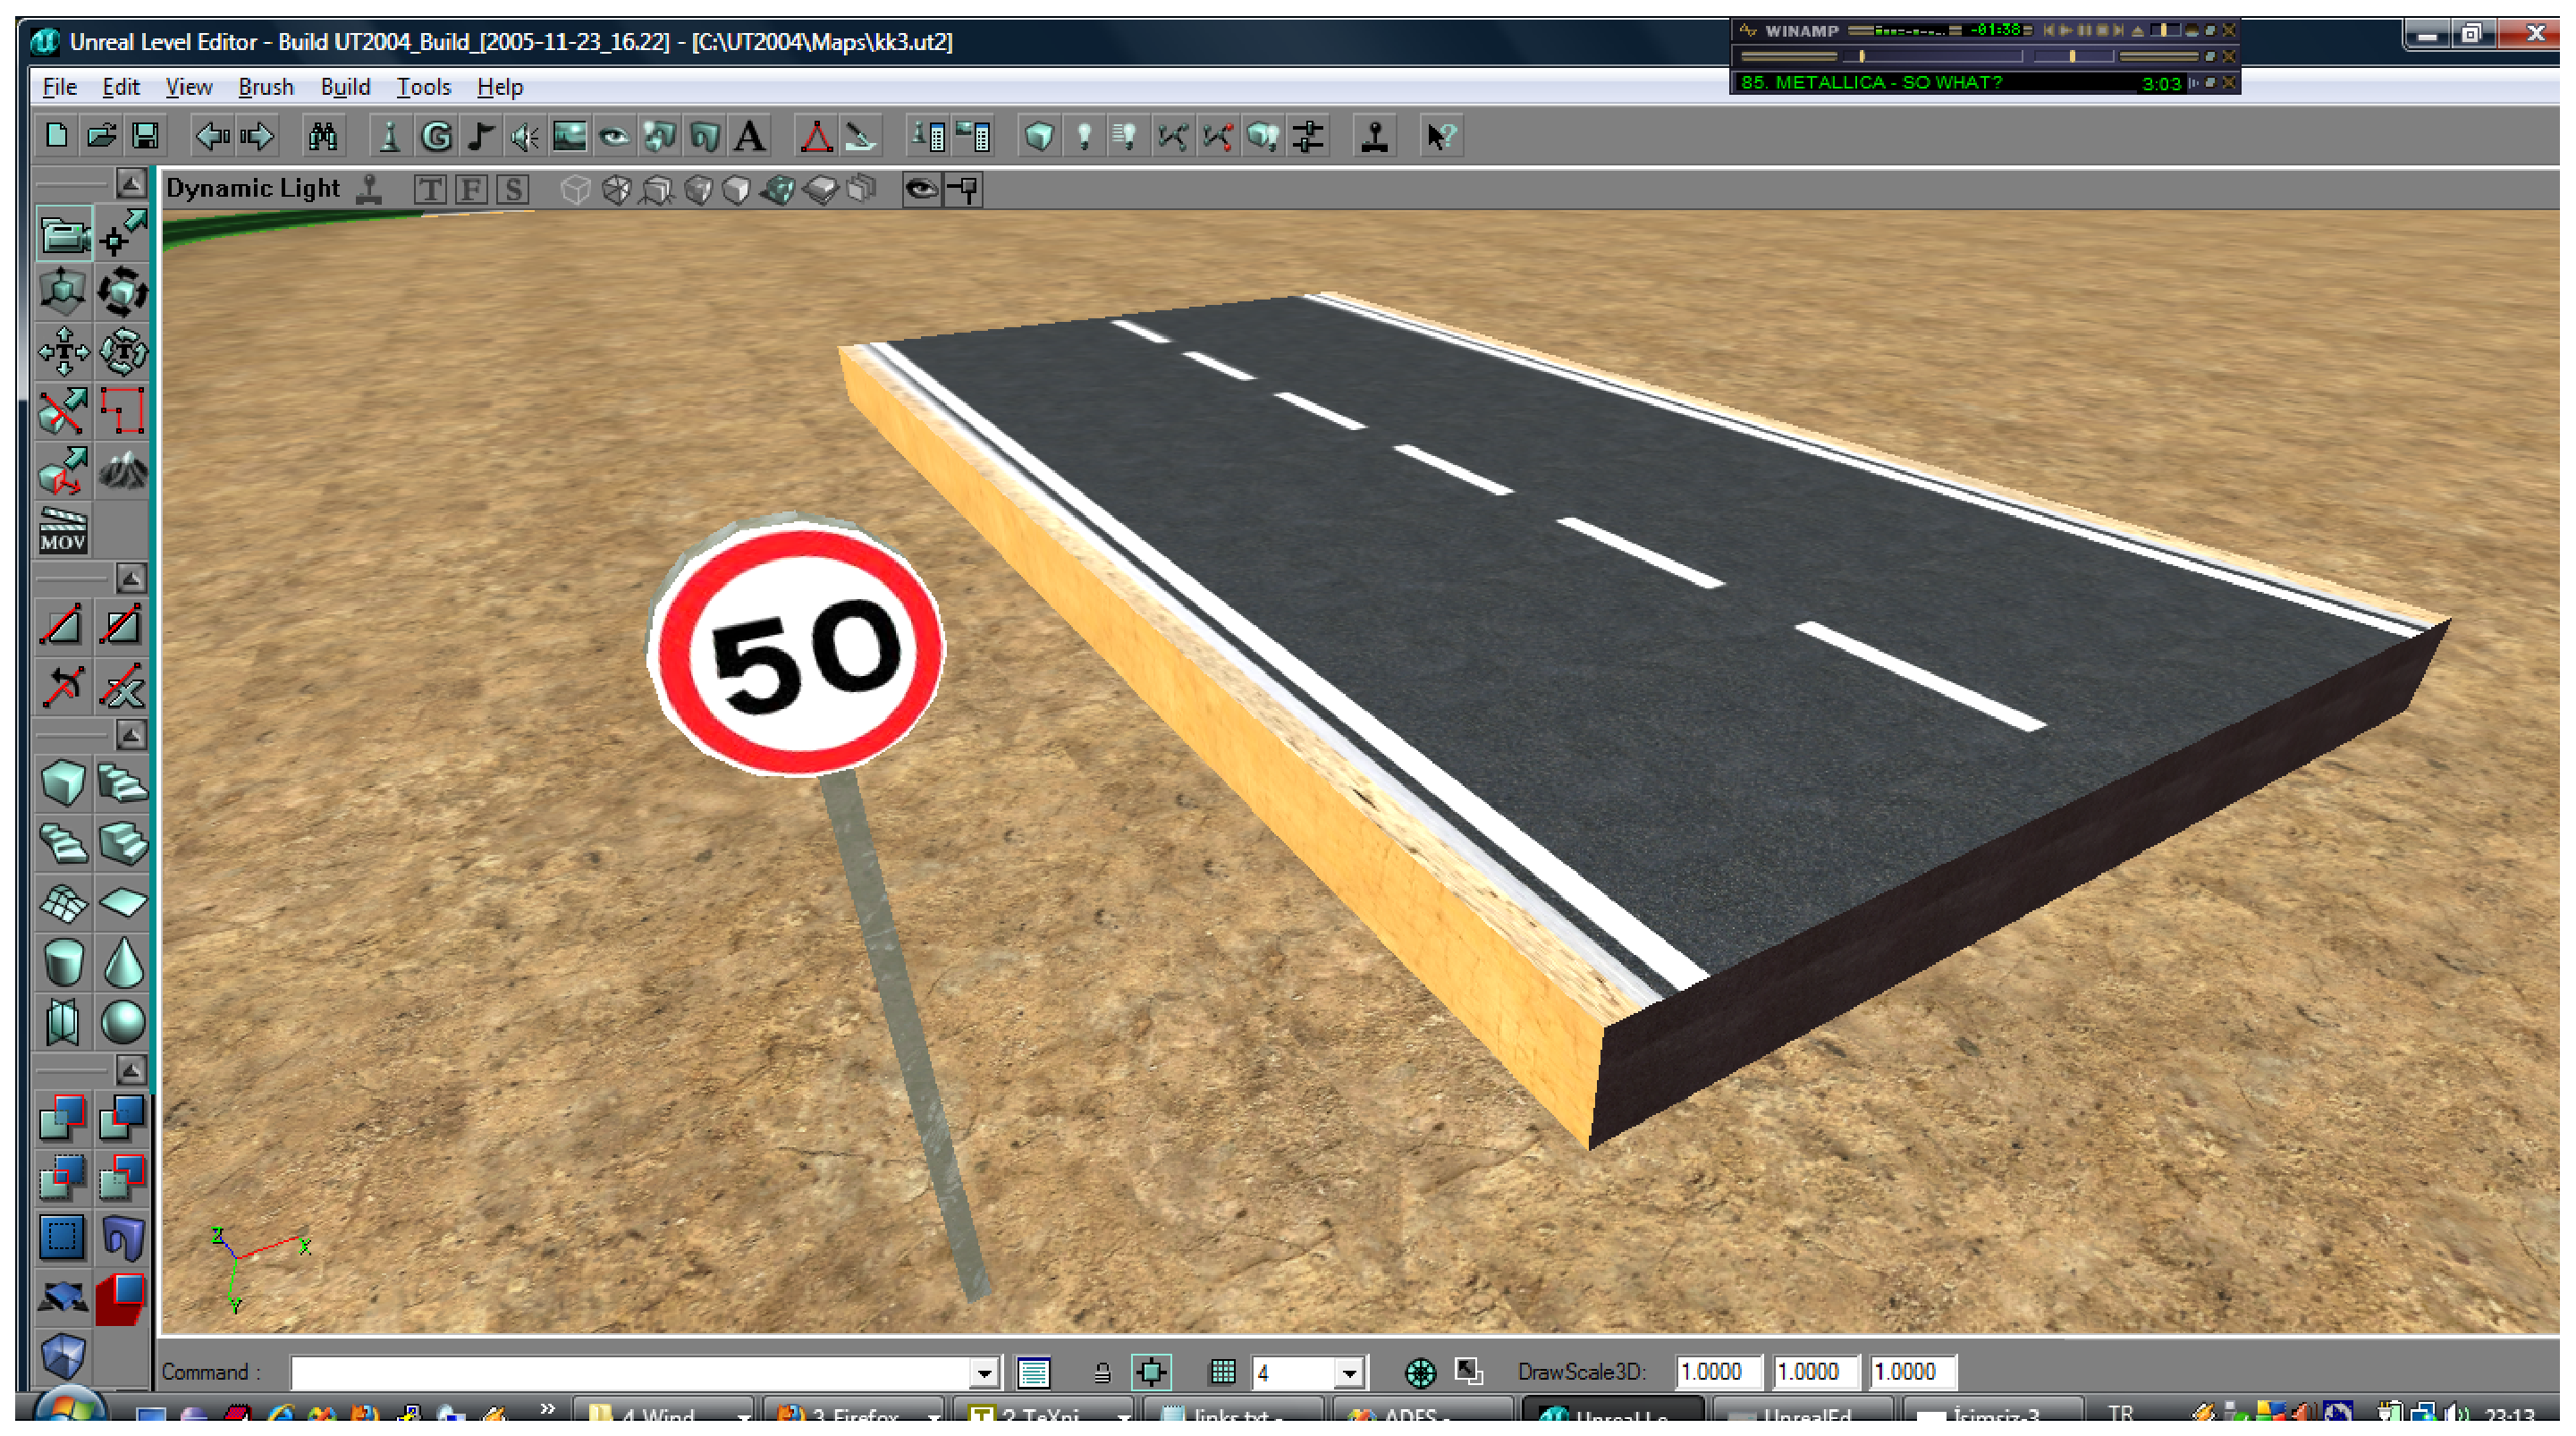
\includegraphics[width=.6\paperwidth]{../img/StaticMesh.eps}
	\caption{Road segment and speed limit sign static meshes.}
	\label{fig:StaticMesh}
	\end{center}
	\end{figure}
\end{frame}

\begin{frame}
	\frametitle{UnrealEd - Terrain/Zone Info}
	\begin{figure}[ht]
	\begin{center}
	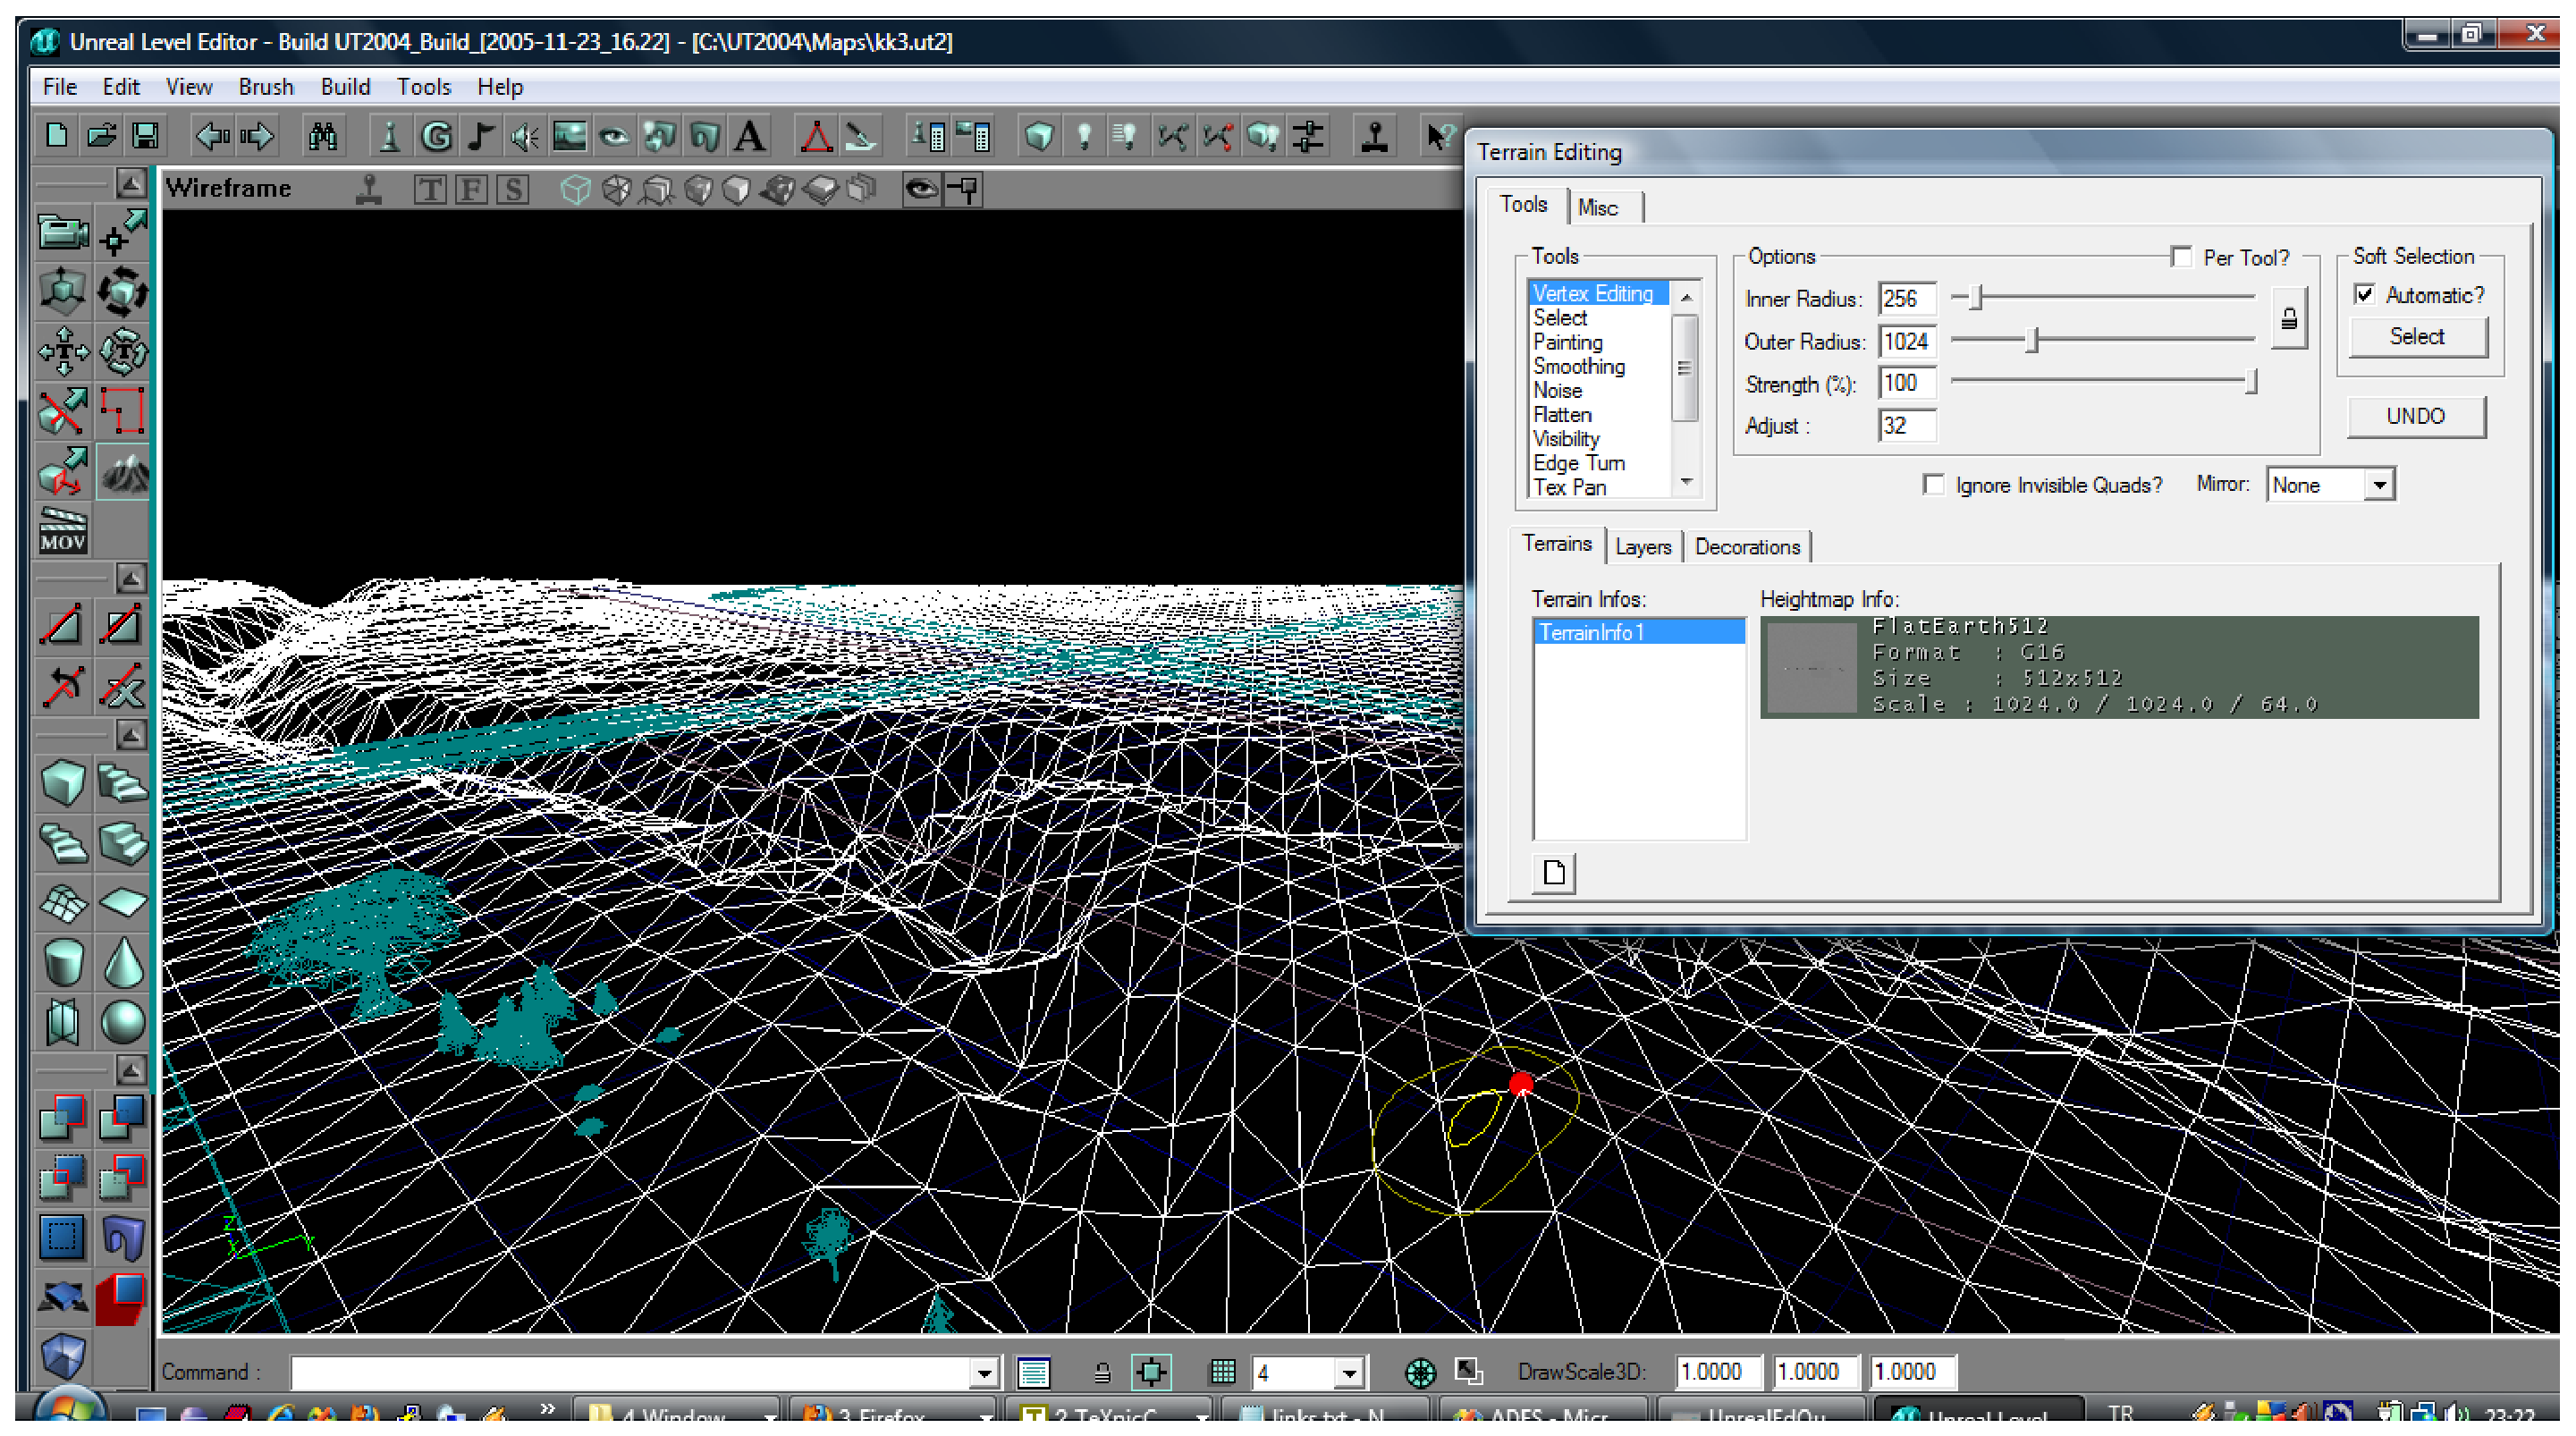
\includegraphics[width=.6\paperwidth]{../img/Terrain.eps}
	\caption{The wireframe of the terrain of the ADES Unreal world.}
	\label{fig:Terrain}
	\end{center}
	\end{figure}
	\begin{block}{}
		ZoneInfo class is used for misc. effects like zone lighting, ambient sound effects, fog effects.
	\end{block}
\end{frame}

\begin{frame}
	\frametitle{UnrealEd - Sky Box}
	\begin{figure}[ht]
	\begin{center}
	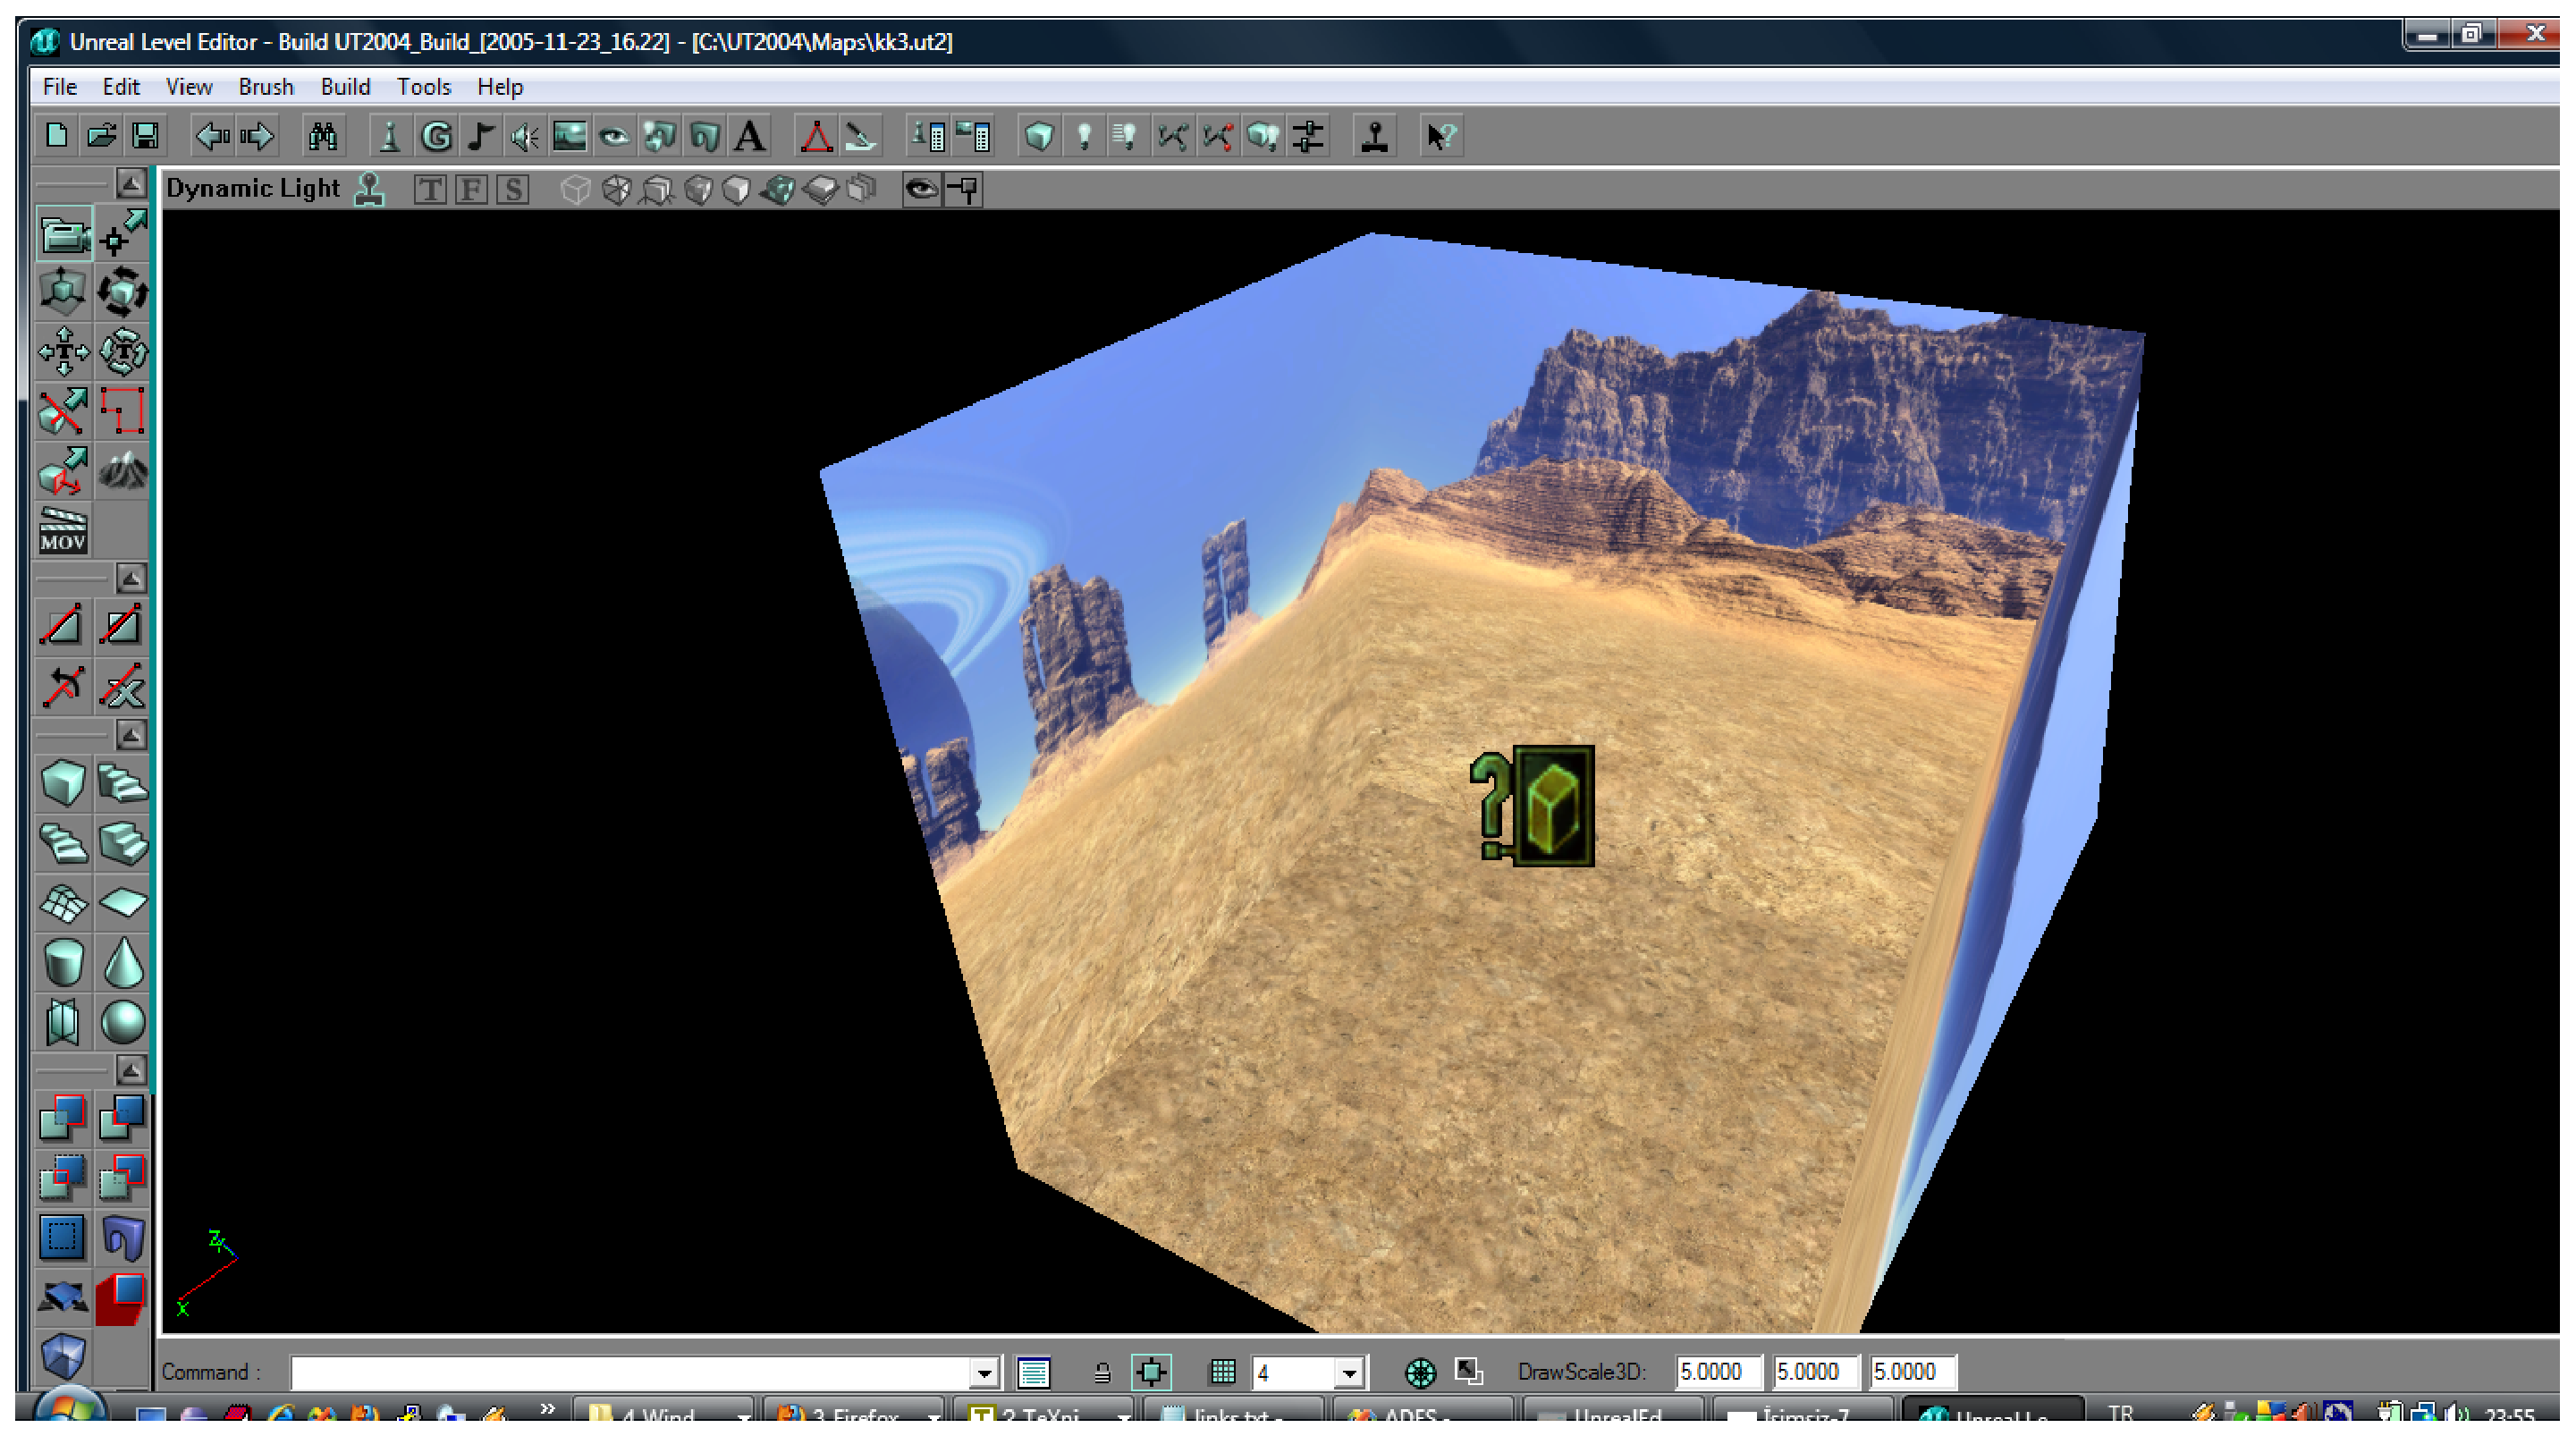
\includegraphics[width=.6\paperwidth]{../img/SkyBox.eps}
	\caption{The SkyBox of the ADES Unreal world.}
	\label{fig:SkyBox}
	\end{center}
	\end{figure}
\end{frame}

\begin{frame}
	\frametitle{UPISEX}
	\begin{block}{}
		UPISEX is a wrapper project for USARSim's image server UPIS for making it visible for .NET projects.
	\end{block}
	\begin{itemize}
	    \item Creates the Unreal Client with Detours hook.
	    \item UPIS captures DirectX specific calls to reach client's memory blocks.
	    \item UPIS opens a TCP/IP port for serving the client's video stream.
	\end{itemize}
\end{frame}

\begin{frame}
	\frametitle{ADES Unreal Controller} 
	\begin{figure}[ht]
	\begin{center}
	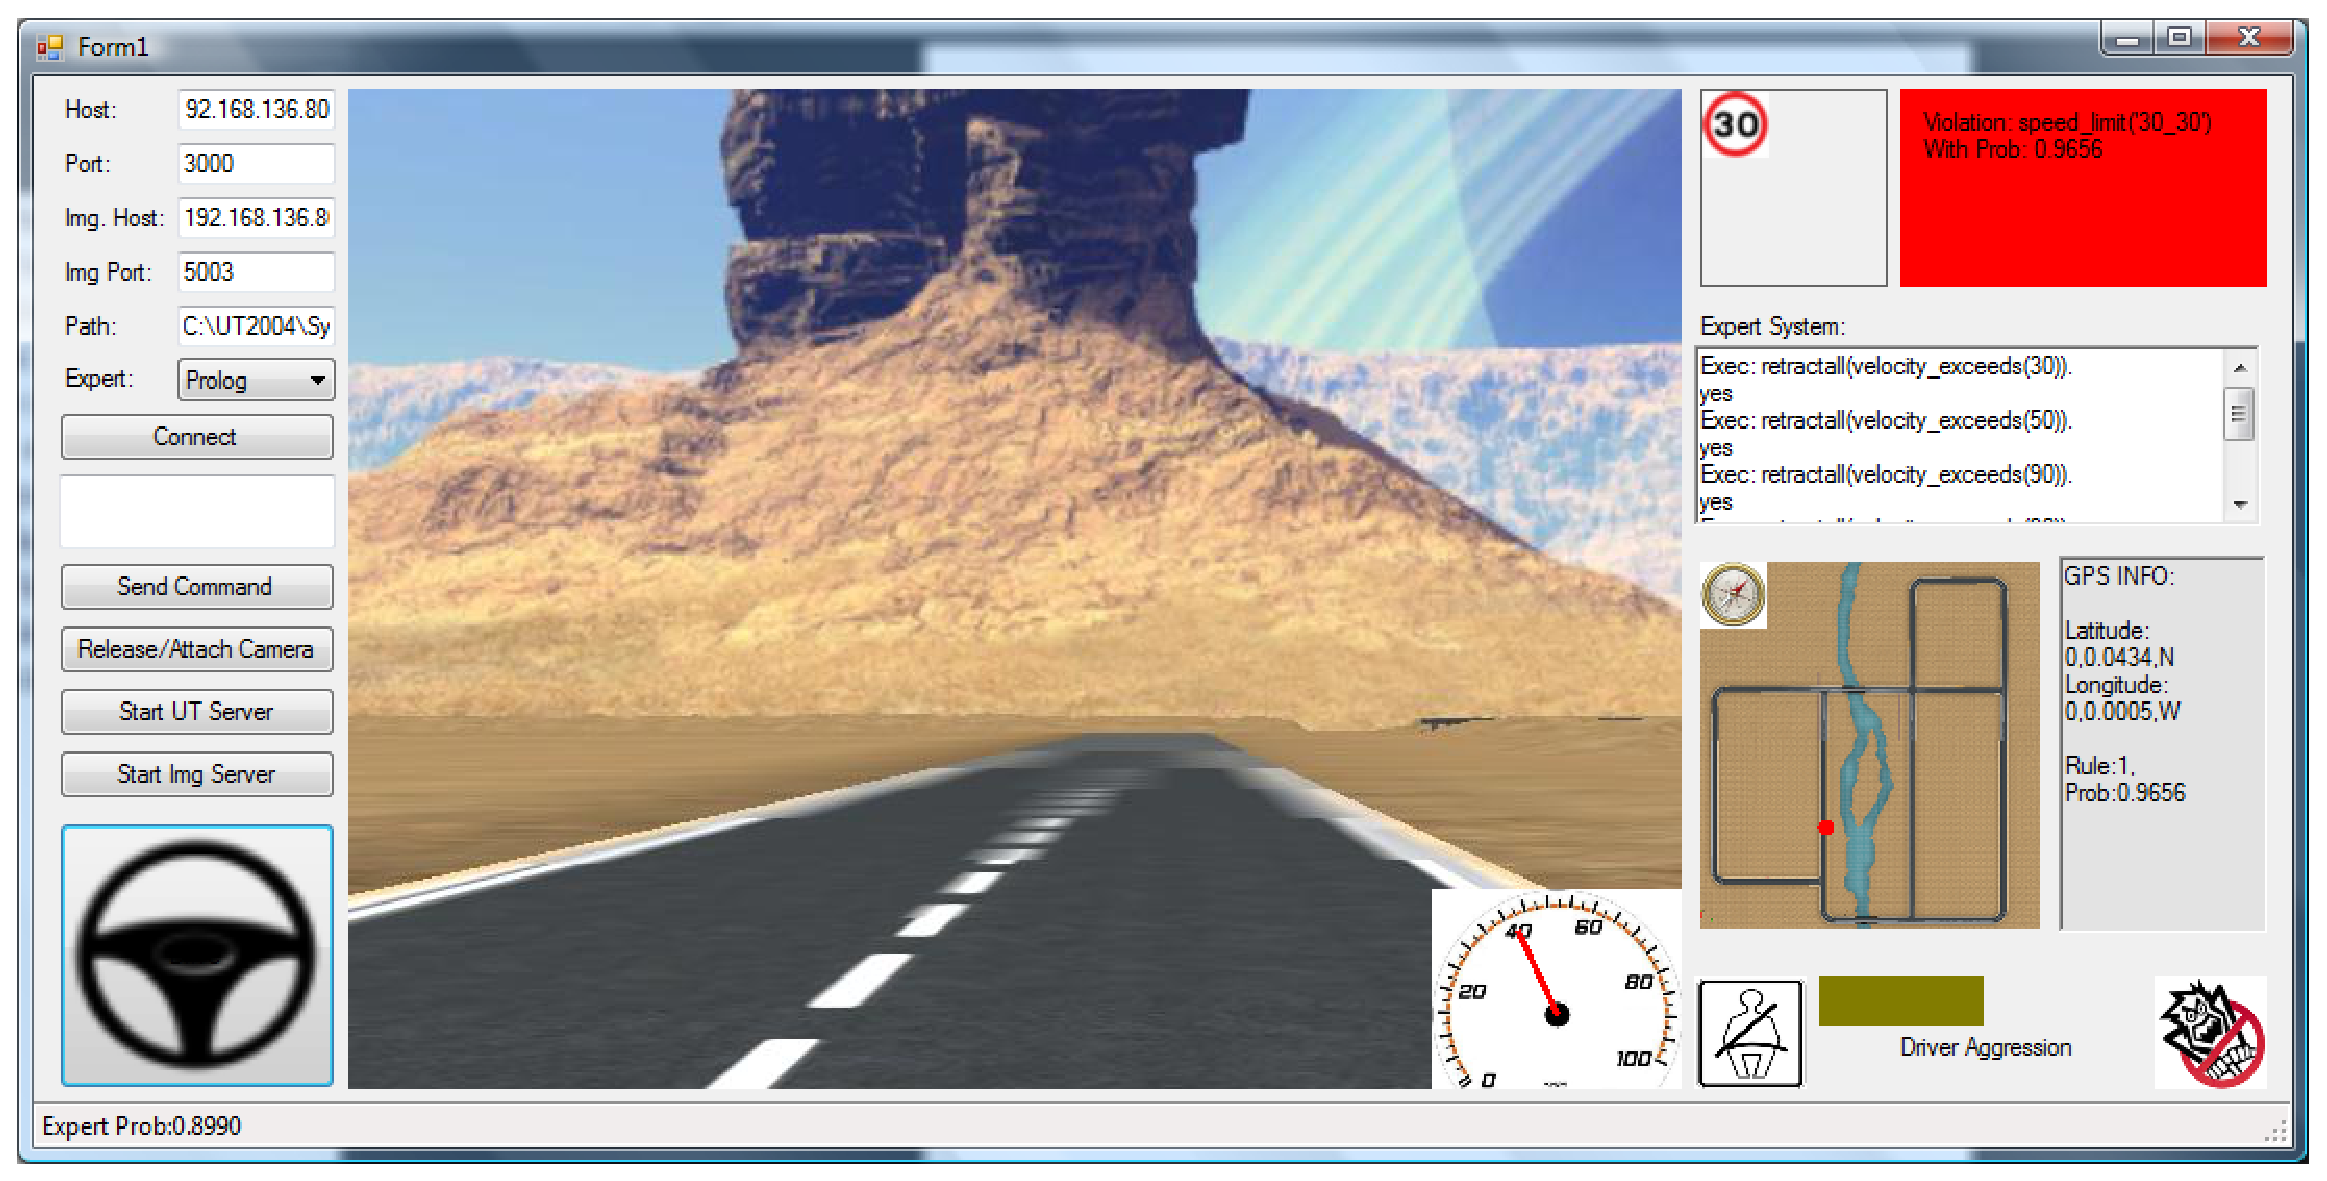
\includegraphics[width=.7\paperwidth]{../img/ADESController.eps}
	\caption{The Unreal ADES controller application interface.}
	\label{fig:ADESController}
	\end{center}
	\end{figure}
\end{frame}

\section{TESTS AND EVALUATION}
\mysectionpage{TESTS AND EVALUATION}{TESTS AND EVALUATION}

\begin{frame}
	\frametitle{Evaluation of Lane Detection} 
	\begin{figure}[ht]
	\begin{center}
	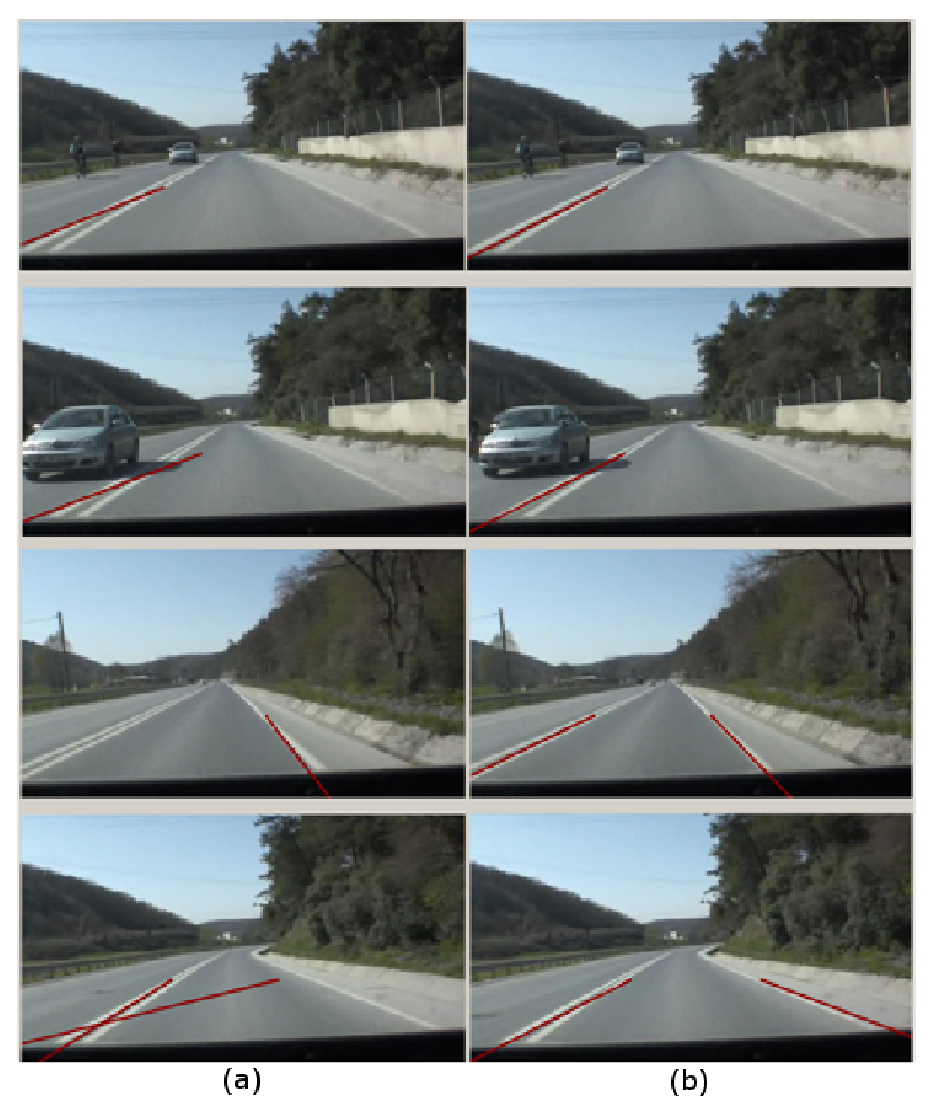
\includegraphics[height=.6\paperheight]{../img/ldfig4.eps}
	\caption{Differences between classical Hough transformation and proposed approach.}
	\label{fig:ldfig4}
	\end{center}
	\end{figure}
\end{frame}

\begin{frame}
	\frametitle{Evaluation of Sign Detection} 
	\begin{table}[ht]
	\centering
	\caption{Detection rate of circular signs.}
	\label{signdetect-table-1}
	{\footnotesize
	\begin{tabular}{|l r r r r|}
		\hline
		\textbf{Fitness threshold} 		& 30 & 30 & 30 & 35 \\
		\textbf{Population size} 			& 60 & 120 & 60 & 60 \\
		\textbf{Number of Generations} 	& 2 & 2 & 4 & 2 \\
		\textbf{Mutation rate}     		& 0.35 & 0.35 & 0.35 & 0.35 \\
		\textbf{Crossover rate} 				& 0.75 & 0.75 & 0.75 & 0.75 \\
		\textbf{Selection method} 				& Elitist & Elitist & Elitist & Elitist \\
		\hline
		\textbf{Avg. Process Time(msec)}	& 9 & 14 & 14 & 9 \\
		\textbf{True detections (percent)} &  95 &  96 &  96 &  65 \\
		\textbf{Misses (percent)}	&  5 &  4 &  4 &  35 \\
		\hline
		\textbf{False detections (percent)}				&  5 &  7 &  6 &  1 \\
		\hline
	\end{tabular}
	}
	\end{table}	
\end{frame}

\begin{frame}
	\frametitle{Evaluation of Sign Detection (cont'd)} 
	\begin{table}[ht]
	\centering
	\caption{Detection rate of triangular signs.}
	\label{signdetect-table-2}
	{\footnotesize
	\begin{tabular}{|l r r r r|}
	\hline
	\textbf{Fitness threshold} 		& 16 & 16 & 16 & 12 \\
	\textbf{Population size} 			& 60 & 150 & 60 & 60 \\
	\textbf{Number of Generations} 	& 2 & 2 & 6 & 2 \\
	\textbf{Mutation rate}     		& 0.35 & 0.35 & 0.35 & 0.35 \\
	\textbf{Crossover rate} 				& 0.75 & 0.75 & 0.75 & 0.75 \\
	\textbf{Selection method} 				& Elitist & Elitist & Elitist & Elitist \\
	\hline
	\textbf{Avg. Process Time(msec)}			& 9 & 16 & 14 & 9 \\
	\textbf{True detections (percent)}				& 87 & 88 & 90 & 94 \\
	\textbf{Misses (percent)}				&  13 & 12 & 10 & 6 \\
	\hline
	\textbf{False detections (percent)}				&  4 &  4 &  5 &  9 \\
	\hline
	\end{tabular}
	}
	\end{table}
\end{frame}

\begin{frame}
	\frametitle{Evaluation of Sign Classification} 
	\begin{table}[ht]
	\centering
	\caption{Classification success rate of circular signs.}
	\label{signclassify-table-1}
	\begin{tabular}{|l r r|}
	\hline
	\textbf{Classification Method} & NN & SVM \\
	\hline
	\textbf{Avg. Process Time(msec)}			& 5 & 10 \\
	\textbf{Error rate (percent)}				& 9 &  20 \\
	\hline
	\end{tabular}
	\end{table}
	\begin{table}[ht]
	\centering
	\caption{Classification success rate of triangular signs.}
	\label{signclassify-table-2}
	\begin{tabular}{|l r r|}
	\hline
	\textbf{Classification Method} & NN  & SVM  \\
	\hline
	\textbf{Avg. Process Time(msec)}			& 3 & 6 \\
	\textbf{Error rate (percent)}				&  7 &  9 \\
	\hline
	\end{tabular}
	\end{table}	
\end{frame}

\begin{frame}
	\frametitle{Evaluation of Sign Recognition System} 
	\begin{table}[ht]
	\centering
	\caption{Overall system performance.}
	\label{signdetection-overall}
	\begin{tabular}{|l|r r|}
	\hline
	& \multicolumn{2}{c|}{CIRCULAR} \\
	\hline
	\textbf{Classification Method} & NN & SVM \\
	\hline
	\textbf{Avg. Process Time(msec)}			& 14 & 19 \\
	\hline
	\textbf{Error rate (percent)}				&  14 &  24 \\
	\hline
	\hline
	& \multicolumn{2}{c|}{TRIANGULAR} \\
	\hline
	\textbf{Classification Method} & NN & SVM \\
	\hline
	\textbf{Avg. Process Time(msec)}			& 12 & 15 \\
	\hline
	\textbf{Error rate (percent)}				&  11 &  13 \\
	\hline
	\end{tabular}
	\end{table}	
\end{frame}

\begin{frame}
	\frametitle{Evaluation of Sign Recognition System (cont'd)} 
	\begin{table}
	\centering
	\caption{Comparison with selected methods from the last decade.}
	\label{tab:perf}
	{\tiny
	\begin{tabular}{|p{14mm}|p{12mm}|l|l|r|r|p{10mm}|}
	\hline
	{\bf Method} & {\bf Reference} & {\bf Year} & {\bf Hardware} & {\bf Image Size (px)} & {\bf Time (msec)} & {\bf Success Rate (\%)} \\
	\hline
	Matching Pursuit &        Hsu and Huang &       2000 &   Intel P2 &    512x480 &       ~250 &   up to 88 \\
	\hline
	Genetic Algorithm &   Escalera &       2002 & AMD Duron 1Ghz &    384x286 & ~450 (51x8.8) &        N/A \\
	\hline
	Kalman Filter &       Fang &       2003 & Intel P4 1GHz &    320x240 &      $>$1000 &        N/A \\
	\hline
	Feature Extraction &        Gao &       2005 &   Intel P3 &  1680x1680 &       ~450 &   up to 95 \\
	\hline
	       SVM &     Maldonado-Bascon &       2005 & Intel P4 2.2Ghz &    720x576 &      $>$ 1000 &   up to 93 \\
	\hline
	Geometric Fragmentation &   Soetedjo and Yamada &       2005 & Intel P4 2.6 GHz &    240x180 &       ~750 &   up to 86 \\
	\hline
	Haar Wavelet Features &   Bahlmann &       2005 & Intel Xeon 2.8Ghz &    384x288 &       ~100 &         85 \\
	\hline
	Neural Networks &      Nguwi and Kouzani &       2006 & Pentium M 1.7Ghz &        N/A &       ~550 &   up to 95 \\
	\hline
	  Adaboost &       Baro &       2007 &        N/A & 60x60 stereo &      $>$ 1000 &      87-90 \\
	\hline
	Color Distance Transform &       Ruta &       2007 &        N/A &    640x480 &        ~35 &   up to 85 \\
	\hline
	Affine Trans., GA, NN & Proposed Approach &       2010 & Intel T5450 1.66Ghz &    512x288 &        ~13 &         87 \\
	\hline
	\end{tabular}  
	}
	\end{table}	
\end{frame}

\begin{frame} [fragile]
	\frametitle{Output of Prolog Based ES } 
	\begin{figure}
	\begin{mylisting}
	Prolog based expert system
	\vspace*{2px}\hrule
	\begin{verbatim}
	Exec: assert("1.0000::T::sign_detected(speed_limit,30)").
	Exec: retractall(velocity_exceeds(X)).
	Exec: retractall(velocity_exceeds(50)).
	Exec: assert("1::T::velocity_exceeds(50)").
	Exec: violation(V,A,P).
	Exec: retractall(gps_node_property(speed_limit,30)).
	Exec: assert("0.9577::T::gps_node_property(speed_limit,30)").
	Exec: retractall(velocity_exceeds(X)).
	Exec: retractall(velocity_exceeds(50)).
	Exec: assert("1::T::velocity_exceeds(50)").
	Exec: violation(V,A,P).
	P = 0.957698767978062
	V = speed_limit
	A = '50_30'
	\end{verbatim}
	\end{mylisting}
	      \caption{Speed violation output of Prolog based expert system.}
	      \label{output1}
	\end{figure}	
\end{frame}

\begin{frame}
	\frametitle{Output of Prolog Based ES (cont'd)} 
	\begin{equation}
	\label{eq13}
		p_{v} = (p_{d} \times \alpha_{d} )(p_{s} \times \alpha_{s} )(p_{g} \times \alpha_{g})
	\end{equation}
	\begin{block}{}	
	Note: The probabilities of the facts are decreasing by the time!
	\end{block}
\end{frame}

\begin{frame} [fragile]
	\frametitle{Output of BN Based ES } 
	\begin{figure}
	\begin{mylisting}
	BN based expert system
	\vspace*{2px}\hrule
	\begin{verbatim}
	SpeedLimit:Vehicle_Speed()->(0,1,0,0)
	SpeedLimit belief: 0.5436
	SpeedLimit:GPS_Node_Property()->(0.0333,0.0333,0.0333,0.9)
	SpeedLimit:Sign_Detected()->(1,0,0,0)
	SpeedLimit:Vehicle_Speed()->(0,1,0,0)
	SpeedLimit belief: 0.5436
	SpeedLimit:GPS_Node_Property()->(0.9708,0.0097,0.0097,0.0097)
	SpeedLimit:Vehicle_Speed()->(0,1,0,0)
	SpeedLimit belief: 0.9491
	\end{verbatim}
	\end{mylisting}
	      \caption{Speed violation output of BN based expert system.}
	      \label{output2}
	\end{figure}
\end{frame}

\begin{frame}
	\frametitle{Output of BN Based ES (cont'd)} 
	{\footnotesize
	\begin{equation}
	\label{eq14}
		p_{v} = \sum_{d\in{Sign\_Detected},s\in{Vehicle\_Speed},g\in{GPS_Node_Property}}p_{d} \times p_{s} \times p_{g} \times vp(d,s,g)
	\end{equation}
	}	
	For the previous output;
	\begin{eqnarray}
	\label{eq15}
	p_{v} &=& 0.9708 \times 1 \times 1 \times 0.9570 \\
	\nonumber & & + 0.00973 \times 1 \times 1 \times 0.7660  \\
	\nonumber & & + 0.00973 \times 1 \times 1 \times 0.7870  \\
	\nonumber & & + 0.00973 \times 1 \times 1 \times 0.5110  \\
	\nonumber p_{v} &=& 0,94913832
	\end{eqnarray}
\end{frame}

\section{CONCLUSION}
\mysectionpage{CONCLUSION}{CONCLUSION}

\begin{frame}
	\frametitle{Key Contributions} 
	\begin{itemize}
	\item The selected point based image binarization, 
	\item The MHT-HMM lane detection, 
	\item The GA and affine transformation based sign detection mechanism, 
	\item The RFID and GPS data structures, 
	\item The enhanced Prolog engine with probabilistic and time-decaying facts, 
	\item Application of BN to driver evaluation system,
	\item The applications for real and simulated environments.
  \end{itemize}
\end{frame}	

\begin{frame}
	\frametitle{Future Works} 
	Not limited to;
	\begin{itemize}
	\item End-to-end implementation of the application for the real environment,
	\item Self modifying, or learning, inference engine,
	\item Improved sensor processor modules for given modules,
	\item Integration of advance vision processing modules,
	\item Wireless integration of the system to the traffic control center,
	\item More vehicle to vehicle and vehicle to infrastructure communication,
	\item Integration with existing intelligent highway systems.
  \end{itemize}	
\end{frame}	

\begin{frame}
	\frametitle{Acknowledgements} 
	I would like to thank to my thesis supervisor Professor Levent Ak{\i}n, my committee, Assoc. Prof. Tankut Acarman, Prof. G\"okmen Erg\"un, Prof. Cem Say, and Prof. O\u{g}uz Tosun, the past and present members of the Robotics Group of  Bo{\u g}azi{\c c}i University Artificial Intelligence Laboratory, and finally my family for their never ending support.
\end{frame}	

\mysectionpage{QUESTIONS?}{Kemal Kaplan\\kaplanke@boun.edu.tr}

\end{document}
